\chapter{发 热}

\section{【发热的定义与病因】}

正常人的体温在体温调节中枢的调节下,产热与散热处于动态平衡之中,维持人体的体温在相对恒定的范围之内。口腔温度(舌下测温)范围约为36.3~37.2℃,直肠内温度一般比口腔约高0.3~0.5℃,腋窝温度比口腔约低0.2~0.4℃。

在生理状态下,不同的个体,同一个体不同的时间和不同的环境,其体温会有所不同:①不同个体:儿童由于代谢率高,体温可比成年人高;老年人代谢率低,体温比成年人低;个别人的基础体温可比正常范围略高或略低0.5℃左右。②同一个体不同时间:正常情况下,人体体温在早晨较低,下午较高,但一般波动范围不超过1℃;妇女在排卵期和妊娠期体温较高,月经期较低。③不同环境:运动、进餐、情绪激动和高温环境下工作时体温较高,低温环境下体温较低。

在病理状态下,由于各种不同原因致人体产热增多或(及)散热减少,使体温升高超过正常范围时,就称为发热。一般来说,口腔温度在37.3℃以上,或直肠温度在37.6℃以上,可认为有发热。临床上按热度高低将发热分为低热(37.3~38℃)、中等度热(38.1~39℃)、高热(39.1~41℃)及超高热(41℃以上)。

引起发热的病因很多,按有无病原体侵入人体分为感染性发热和非感染性发热两大类。

\subsection{(一)感染性发热}

引起感染性发热的病原体有细菌、病毒、支原体、立克次体、螺旋体、真菌及寄生虫等。各种病原体侵入人体后可引起相应的疾病,不论急性还是慢性、局灶性还是全身性均可引起发热。病原体及其代谢产物或炎性渗出物等外源性致热原,在体内作用于致热原细胞如中性粒细胞、单核细胞-巨噬细胞等,使其产生并释放白细胞介素-1、干扰素、肿瘤坏死因子及炎症蛋白-1等而引起发热。感染性疾病占发热病因的50\%~60\%。

\subsection{(二)非感染性发热}

由病原体以外的其他病因引起的发热称为非感染性发热。常见于以下原因:

\subsubsection{1.吸收热}

由于组织坏死、组织蛋白分解和坏死组织吸收引起的发热称为吸收热。

\paragraph{(1)物理和机械性损伤:}

大面积烧伤、创伤、大手术后、骨折、内脏出血和热射病等。

\paragraph{(2)血液系统疾病:}

白血病、恶性淋巴瘤、恶性组织细胞病、骨髓增生异常综合征、多发性骨髓瘤、急性溶血、血型不合输血等。

\paragraph{(3)肿瘤性疾病:}

血液恶性肿瘤之外的各种恶性肿瘤。

\paragraph{(4)血栓栓塞性疾病:}

①静脉血栓形成:如股静脉血栓形成。②动脉血栓形成:如心肌梗死、肺动脉栓塞。③微循环血栓形成:如血栓性血小板减少性紫癜、弥散性血管内凝血等。

\subsubsection{2.变态反应性发热}

变态反应产生的抗原抗体复合物成为外源性致热原,激活了致热原细胞,使其产生并释放白细胞介素-1、干扰素、肿瘤坏死因子及炎症蛋白-1等引起的发热。如风湿热、药物热、血清病以及各种结缔组织病(如系统性红斑狼疮、多发性肌炎与皮肌炎、结节性多动脉炎等)。

\subsubsection{3.中枢性发热}

有些致热因素不通过内源性致热原而直接损害体温调节中枢,使体温调定点上移后发出调节冲动,造成产热大于散热,体温升高,称为中枢性发热。这类发热的特点是高热无汗。如:

(1)物理因素:如中暑等。

(2)化学因素:如重度安眠药中毒等。

(3)机械因素:如颅内出血或颅内肿瘤细胞浸润等。

(4)功能性因素:如自主神经功能紊乱和感染后低热等。

\subsubsection{4.其他}

如甲状腺功能亢进、痛风、严重脱水、因致热原引起的输液或输血反应等。

\section{【发热疾病的检查】}

\subsection{(一)问诊}

发热的病因复杂,常造成诊断上的困难。认真细致的问诊常能为进一步检查提供重要提示。问诊的要点包括:①起病时间、季节、起病情况(缓急)、病程、程度(热度高低)、频度(间歇性或持续性)、诱因。②有无畏寒、寒战、大汗或盗汗。③多系统症状询问,如是否伴有皮疹、出血、黄疸、咳嗽、咳痰、咯血、胸痛、腹痛、呕吐、腹泻、尿频、尿急、尿痛、头痛、肌肉关节痛等。④患病以来一般情况,如精神状态、食欲、体重改变及睡眠。⑤诊治经过(拟诊、药物、剂量、疗效)。⑥传染病接触史、疫水接触史等流行病学资料;手术史、流产或分娩史、用药史、职业特点等。兹就其中一些重要问题再强调如下:

\subsubsection{1.病史}

详细询问病史往往为发热的诊断与鉴别诊断提供重要线索。例如传染病的流行病学资料十分重要,如蚊虫叮咬可引起乙型脑炎、疟疾、登革热等;有牧区逗留与牲畜接触史者可患布鲁菌病;1个月内有血吸虫病疫水接触史者可引起急性血吸虫病。发热前2~3周内有无皮肤外伤及疖肿史,如有是诊断葡萄球菌败血症的重要线索。在用药过程中出现原因未明发热要注意药物热的可能。大量使用广谱抗生素、糖皮质激素、免疫抑制剂等引起二重感染(机会感染)而致发热不退,或热退后又再发热者亦时有见之。

\subsubsection{2.发热的特点}

\paragraph{(1)发热的临床过程和特点:}

1)体温上升期:体温上升有两种方式:①骤升型:体温在几小时内达39℃以上,常伴有寒战。见于疟疾、大叶性肺炎、败血症、流行性感冒、急性肾盂肾炎、输液或输血反应等。②缓升型:体温逐渐上升在数日内达高峰,多不伴寒战。如伤寒、结核病、布鲁菌病等所致的发热。

2)高热期:是指体温上升达高峰之后保持一定时间。不同疾病持续时间长短不等。如疟疾可持续数小时,大叶性肺炎、流行性感冒可持续数天,伤寒则可长达数周。

3)体温下降期:①骤降型:指体温于数小时内迅速下降至正常,有时可略低于正常,常伴有大汗淋漓。常见于疟疾、急性肾盂肾炎、大叶性肺炎和输液反应等。②渐降型:指体温在数天内逐渐降至正常,如伤寒、风湿热等。

\paragraph{(2)热型:}

不同病因所致发热的热型也常不同:

1)稽留热:体温恒定地维持在39~40℃以上的高水平,达数天或数周。24小时内体温波动范围不超过1℃。常见于大叶性肺炎、恙虫病、流行性脑脊髓膜炎、斑疹伤寒及伤寒的高热期。

2)弛张热:又称败血症热型。体温常在39℃以上,24小时内体温波动范围超过2℃,但都在正常水平以上。常见于败血症、风湿热、重型肺结核及化脓性炎症等。

3)间歇热:体温骤升达高峰后持续数小时,然后迅速降至正常水平,无热期(间歇期)可持续1至数天。如此高热期与无热期反复交替出现。可见于疟疾、急性肾盂肾炎、淋巴瘤、败血症等。

4)波状热:体温逐渐上升达39℃或以上,数天后又逐渐下降至正常水平,持续数天后又逐渐升高,如此反复多次。常见于布鲁菌病、登革热等。

5)回归热:体温急骤上升至39℃或以上,持续数天后又骤然回复到正常水平,高热期与无热期各持续若干天后规律性交替1次。可见于回归热、霍奇金淋巴瘤、周期热等。

6)不规则热:发热的体温曲线无一定规律,可见于结核病、风湿热、支气管肺炎、渗出性胸膜炎、流行性感冒、败血症等。

一般说来,热程短、高热、寒战等中毒症状者,有利于感染性疾病的诊断;如热程中等,但呈渐进性消耗、衰竭者,以结核和恶性肿瘤多见;热程长,无毒血症状,发作与缓解交替出现,则有利于结缔组织病的诊断。

\subsubsection{3.发热的伴随症状}

\paragraph{(1)寒战:}

常见于大叶性肺炎、败血症、急性肝胆道感染、急性肾盂肾炎、流行性脑脊髓膜炎、疟疾、钩端螺旋体病、药物热、急性溶血、输血或输液反应等。

\paragraph{(2)全身状况:}

渐进性消瘦衰竭见于结核、恶性肿瘤等;不少结缔组织病早期精神、食欲及体重可无明显变化。

\paragraph{(3)各系统症状:}

可提示疾病的部位。皮疹与多种急性发热性疾病(参见第2节)和慢性发热性疾病相关。

\subsection{(二)体格检查}

全面而细致的体格检查非常重要,兹重点讨论如下:

\subsubsection{1.一般状况及全身皮肤黏膜检查}

注意全身营养状况。恶病质提示重症结核、恶性肿瘤。注意有无皮疹及皮疹类型:斑疹见于斑疹伤寒、丹毒;面部蝶形红斑、指端及甲周红斑提示为系统性红斑狼疮;环形红斑见于风湿热;丘疹和斑丘疹见于猩红热、药物热;玫瑰疹见于伤寒和副伤寒。睑结膜及皮肤少许瘀点,指端、足趾、大小鱼际肌有压痛的Osler小结节见于亚急性感染性心内膜炎;软腭、腋下条索状或抓痕样出血点见于流行性出血热;耳廓、跖趾、掌指关节等处结节为痛风石,见于痛风患者;皮肤散在瘀点、瘀斑、紫癜见于再生障碍性贫血、急性白血病及恶性组织细胞瘤;大片瘀斑提示弥散性血管内凝血。皮肤和软组织的化脓性病灶,常为发热病因,或败血症的来源。皮肤巩膜出现黄疸提示肝、胆道疾病、溶血性疾病和中毒性肝损害。

\subsubsection{2.淋巴结检查}

注意全身浅表淋巴结有无肿大。局部淋巴结肿大、质软、有压痛者,要注意相应引流区有无炎症。局部淋巴结肿大、质硬、无压痛,可能为癌肿转移;局部或全身淋巴结肿大、质地韧实有弹性、无压痛者可能为淋巴瘤;全身淋巴结肿大尚可见于急慢性白血病、传染性单核细胞增多症、系统性红斑狼疮等。

\subsubsection{3.头颈部检查}

结膜充血多见于流行性出血热、斑疹伤寒、麻疹;扁桃体肿大,其上有黄白色渗出物可以拭去,为化脓性扁桃体炎;外耳道流出脓性分泌物为化脓性中耳炎;乳突红肿伴压痛为乳突炎、鼻窦压痛点有压痛提示鼻窦炎。检查颈部时注意有无阻力,阻力增加或颈项强直提示为脑膜刺激,见于脑膜炎或脑膜脑炎。甲状腺弥漫性肿大、质软(血管杂音)提示为甲状腺功能亢进。

\subsubsection{4.心脏检查}

胸廓隆起常提示心脏肥大;胸骨下段压痛提示白血病、恶性组织细胞病;心脏扩大和新出现的收缩期杂音提示为风湿热;原有心瓣膜病,病程中杂音性质改变,需考虑感染性心内膜炎,应予查超声心动图、血培养。

\subsubsection{5.肺部检查}

一侧肺局限性叩浊、语颤增强,有湿啰音,提示为大叶性肺炎;下胸部或背部固定或反复出现湿啰音,见于支气管扩张伴继发感染;一侧肺下部叩浊、呼吸音及语颤减低,提示胸腔积液;大量积液时患侧胸廓饱满,气管移向健侧,在年轻患者中以结核性胸膜炎多见,也可见于恶性肿瘤侵犯胸膜或结缔组织病。

\subsubsection{6.腹部检查}

右上腹压痛、Murphy征阳性伴皮肤巩膜黄染,提示为胆囊炎、胆石症发热;中上腹明显压痛、胁腹部皮肤见灰紫斑(Grey-Turner征)或脐周皮肤青紫(Cullen征),甚至上腹部可触及肿块,见于坏死性胰腺炎;转移性腹痛伴麦氏点压痛,多为阑尾炎;右下腹或全腹疼痛伴明显压痛,有时在右下腹或脐周扪及腹块,腹壁或会阴部有瘘管并有粪便与气体排出,全身营养较差,可能为克罗恩病;全腹压痛、反跳痛见于腹膜炎;肝大、质硬、表面有结节或巨块,提示为肝癌;肝脾同时肿大,可见于白血病、淋巴瘤、恶性组织细胞病、系统性红斑狼疮、败血症等。季肋点压痛、肾区叩击痛、提示上尿路感染。

\subsubsection{7.四肢检查}

杵状指(趾)伴发热,可见于肺癌、肺脓肿、支气管扩张、感染性心内膜炎等。多关节红肿、压痛见于风湿热、系统性红斑狼疮、类风湿关节炎。化脓性关节炎、结核性关节炎、痛风的早期常侵犯单个关节。发热伴有肌肉疼痛见于许多急性传染病,一般无特征性诊断意义。如腓肠肌剧烈疼痛,甚至不能站立与行走,常提示钩端螺旋体病。多发性肌肉显著疼痛可见于多发性肌炎或皮肌炎。

\subsubsection{8.神经系统检查}

发热伴意识障碍或(及)脑膜刺激征见于中枢神经系统感染、中枢神经系统白血病或其他肿瘤。应注意发热兼有中枢神经系统症状、体征者,不少起源于急性全身感染、内分泌代谢障碍、结缔组织病、中毒等全身性疾病,但这些疾病多有相应病史和临床表现,应注意与中枢神经系统疾病鉴别。

\subsection{(三)实验室及辅助检查}

实验室检查及器械检查可补充病史与体检的不足,尤其对一些仅以发热为主要症状而缺乏明确反映脏器损害的症状和体征的患者,往往有重要的诊断与鉴别诊断意义。血、尿、大便常规与X线胸片属发热的常规检查。血培养应列为未明原因发热的常规检查。其他检查根据临床提示,有针对性地选择应用。

\subsubsection{1.血常规检查}

白细胞计数及分类对发热的鉴别诊断有重要初筛价值。白细胞总数及中性粒细胞升高,提示为细菌性感染,尤其是化脓性感染;也见于某些病毒感染如流行性出血热;成人Still病、风湿热亦有白细胞增多。极度白细胞增多见于白血病及类白血病反应。大多数病毒感染无白细胞增多,甚至减少;这一现象亦可见于某些细菌感染(如伤寒或副伤寒、结核病的某些类型)和某些原虫感染(如疟疾、黑热病)。嗜酸性粒细胞增多见于寄生虫病、变态反应性疾病等;在伤寒时,嗜酸性粒细胞消失是一个有力的诊断支持点,有助于与其他急性传染病鉴别。绝对性淋巴细胞增多,见于传染性单核细胞增多症、传染性淋巴细胞增多症、百日咳、淋巴细胞性白血病等;淋巴细胞减少,见于大多数病毒性感染,如严重急性呼吸综合征(SARS)和高致病性禽流感肺炎等。全血细胞减少伴发热,见于恶性组织细胞病、重型再生障碍性贫血、白细胞减少的急性白血病、全身血行播散性结核病、癌肿骨髓转移、黑热病、艾滋病等。

\subsubsection{2.尿常规检查}

尿中白细胞增多,尤其是出现白细胞管型,提示急性肾盂肾炎;尿中出现红细胞,可见于尿道感染、败血症等。蛋白尿伴或不伴管型尿见于钩端螺旋体病、流行性出血热、系统性红斑狼疮等;蛋白尿也见于轻链型多发性骨髓瘤。

\subsubsection{3.大便常规检查}

隐血试验阳性、大便红、白细胞均提示有胃肠道病变。

\subsubsection{4.X线胸片}

伴有肺部病征的发热是发热的常见病因(参见第3节),且肺结核目前在我国仍然常见,因此X线胸片应列为发热的常规检查。

\subsubsection{5.血培养和骨髓培养}

血培养应列为未明原因发热(尤其具感染性血象者)的常规检查,该检查对败血症、伤寒或副伤寒、布鲁菌病、感染性心内膜炎等疾病的病因学诊断具有决定性意义。骨髓培养可提高诊断的敏感性。对长期使用广谱抗生素、糖皮质激素、免疫抑制剂及化疗药物者,或严重疾病状态全身衰竭患者,要注意真菌或厌氧菌感染的可能,应加做血真菌和厌氧菌培养。

\subsubsection{6.各种传染病的病原学及血清学检查}

目前我国仍有多种传染病流行,这类疾病构成国人急性发热的常见病因。再者,由于早期干预治疗,临床表现常不典型,因此病原学及血清学检查对这类疾病的及早确诊至关重要。可根据流行病学资料及临床表现的提示选择有关检查。

\subsubsection{7.骨髓涂片检查}

原因未明的长期发热(尤其伴进行性贫血者)是骨髓涂片检查的指征。该检查对各种血液病具有确诊的价值。

\subsubsection{8.结缔组织病相关检查}

原因未明的长期发热,疑有结缔组织病者可进行相关检查,包括血沉、C反应蛋白、蛋白电泳、免疫球蛋白、补体等常规项目,以及选择检查各种自身抗体如抗核抗体(ANA)谱、类风湿因子(RF)、抗中性粒细胞胞浆抗体(ANCA)、抗磷脂抗体等。

\subsubsection{9.影像学检查}

除了上述X线胸片作为常规检查外,根据临床提示可选择B超、CT、PET/CT、MRI用于胸、腹及颅内病灶的诊断;X线小肠钡剂造影用于消化道病变诊断;逆行胰胆管造影(ERCP)或磁共振胰胆管成像(MRCP)用于胆道病变诊断。

\subsubsection{10.内镜检查}

包括呼吸内镜(支气管镜、胸腔镜和纵隔镜),消化内镜(胃镜、结肠镜、小肠镜、胶囊内镜等),泌尿内镜(如膀胱镜),耳、鼻、咽喉镜等对诊断均有帮助。

\subsubsection{11.活体组织检查}

淋巴结活检对原因未明长期发热而兼有淋巴结肿大者往往能为诊断提供重要依据,阳性发现对淋巴结结核、淋巴瘤及癌的淋巴结转移有确诊价值。对某些诊断有困难的血液病如淋巴瘤、白血病、恶性组织细胞病、多发性骨髓瘤等骨髓活检可提高检出率。对诊断确有困难而有肝、脾大或腹膜后淋巴结或纵隔淋巴结肿大者,可考虑在B超或CT引导下行肝、脾、淋巴结穿刺或腹腔镜下取活检。支气管镜下病变组织活检对支气管癌及支气管内膜结核有确诊意义。

\subsubsection{12.其他}

疑感染性心内膜炎或心肌病者行超声心动图检查。疑中枢神经系统感染者行脑脊液检查。疑甲亢者行甲状腺功能检查。PPD皮试作为结核病的辅助检查。某些血清肿瘤标志物如AFP、CA19-9、CEA、CA125对消化系恶性肿瘤、PSA对前列腺癌具有辅助诊断价值。炎症标志物对发热的鉴别也有参考价值,如降钙素原、C-反应蛋白等。生化、肝功能、血清酶学检查对内分泌疾病、肝炎、心肌炎或心肌梗死、肌炎的诊断有帮助。

\section{【原因未明发热疾病的诊断性治疗】}

当病因经过各种检查尚难以查明时,在不影响进一步检查的情况下,可按可能性较大的病因进行诊断性治疗,观察治疗的效果,以助诊断。

\subsection{(一)诊断性治疗的原则和意义}

1.诊断性治疗仅适用于那些对拟诊疾病特异性强、疗效确切且安全性高的治疗药物的患者。

2.诊断性治疗一般否定的意义较肯定的意义大。例如患者经予氯喹的正规抗疟疗程仍不能退热,则疟疾的可能性很少,但反之并不尽然。因此,对诊断性治疗的效应要结合多方面作出恰当评价。

3.诊断性治疗剂量应充足,疗程要足,否则无助于判断。

用于诊断性治疗的药物有抗菌药物、抗原虫药物、抗风湿药物、抗肿瘤药物。例如拟诊疟疾用氯喹,拟诊结核予抗结核药物。

\subsection{(二)诊断性治疗注意事项}

应特别指出,诊断性治疗要慎用,使用不当,不但不起作用,反而会给诊断增加困难,甚至加重病情。兹就一些药物的应用强调如下:

\subsubsection{1.糖皮质激素的应用}

不要滥用糖皮质激素,以免改变原来热型和临床表现,给诊断带来困难;长期应用还会加重原有的感染或诱发新的感染,加重病情。因此,只在少数情况下,如高度怀疑为药物热、成人Still病且病情危急时,方可在有经验的医师指导下谨慎使用此类药物。

\subsubsection{2.抗菌药物的应用}

几乎所有的发热常因患者入院前均已接受了时间不等的抗生素治疗,抗生素诊断性治疗因此针对性不强,不仅干扰及时正确诊断治疗,而且容易导致耐药、二重感染或药物热。因此,应严格加以控制。仅对疑为感染性发热且病情危重的高热患者,在必要的实验室检查和各种培养标本采取后,根据初步临床诊断给予经验性抗菌治疗。

\subsubsection{3.退热药的应用}

确诊前使用退热药会改变热型、影响诊断。但对高热中暑、手术后高热、高热谵妄等应采取紧急降温措施。有条件时,可将室温调在27℃左右,采用物理或(及)药物降温,同时注意防止体温骤降伴大量出汗时可能导致的虚脱或休克。

\section{【发热疾病的分组】}

为便于进行鉴别诊断,从发热的缓急、程度、病程、特殊热型以及伴发的主要症状与体征等出发,将发热划分为急性发热、急性发疹性发热、伴有肺部病征的急性发热、周期性发热、长期发热以及慢性微热等6类,将在本章分别讨论,而伴有其他特别体征的发热,请参考各有关章节。

\protect\hypertarget{text00012.html}{}{}

\section{1 急性发热}

临床上一般将热程在2周以内的发热称为急性发热。急性发热临床常见,且不少为高热,其中以急性感染占首位,包括各种病原体引起的传染病,全身或局灶性感染。而各种病原体中又以细菌最为常见,其次为病毒。非感染的急性发热包括变态反应性疾病、风湿性疾病、组织坏死与血液分解产物的吸收、物理与化学因素、血液病与恶性肿瘤等。内科临床常见的急性发热疾病如表\ref{tab2-1}所示。

\begin{table}[htbp]
\centering
\caption{常见急性发热疾病的分类}
\label{tab2-1}
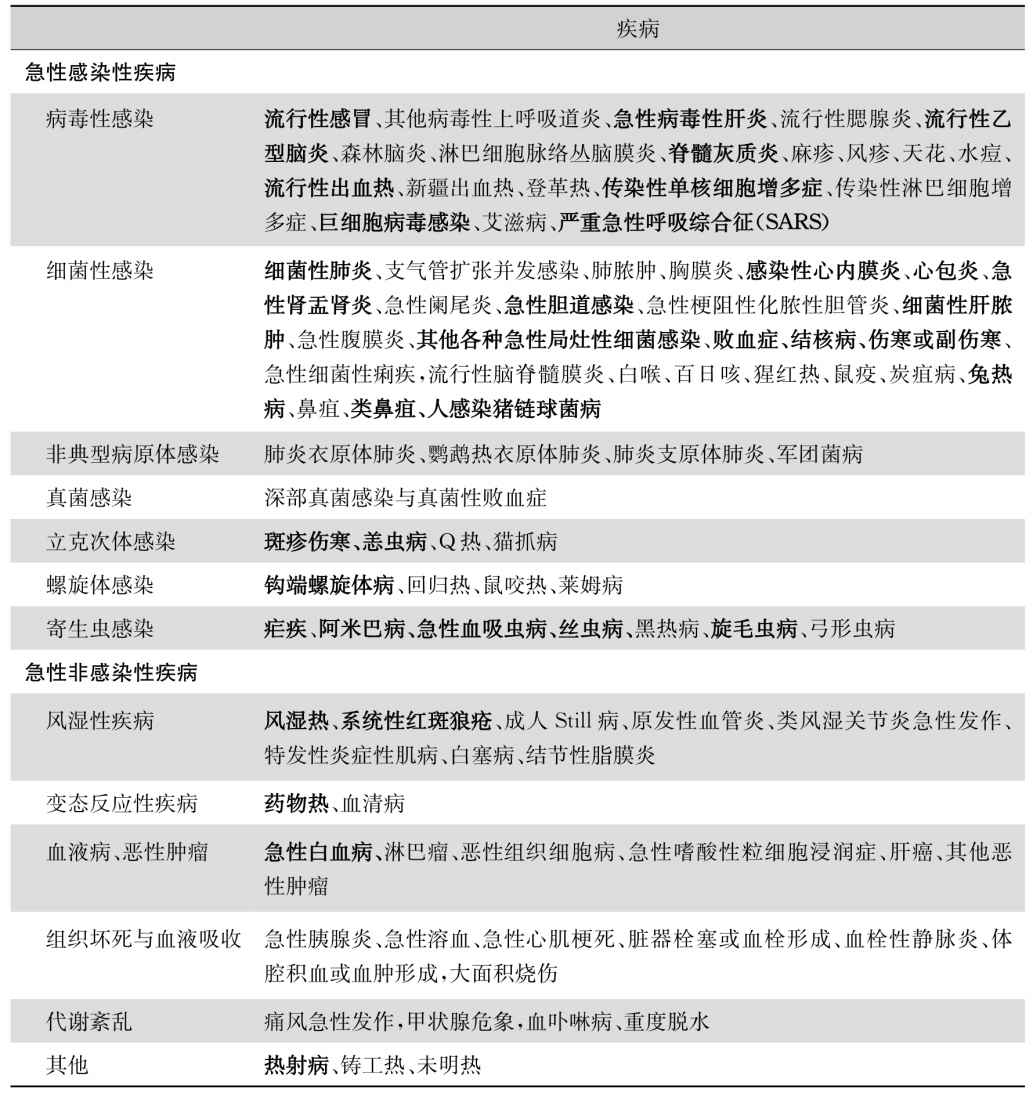
\includegraphics[width=5.92708in,height=6.28125in]{./images/Image00005.jpg}
\end{table}

急性发热性疾病病因很多,病史及临床表现典型者诊断较易,临床表现不典型的病例或较少见的疾病则会造成诊断的困难。因此,对于一时诊断未明的病例,鉴别诊断的思路要广,不但要熟悉常见病,也要了解少见病;不但要知道各种疾病的典型临床表现及实验室和辅助检查的诊断价值,也要不断积累在某特殊情况下临床表现不典型的疾病的诊断经验。本节主要讨论表\ref{tab2-1}中排黑体字的疾病,是在急性发热的鉴别诊断中较常遇到的疾病;以同时伴有皮疹为特征的急性发热性疾病放在“2.急性发疹性发热”一节中讨论;对伴有肺部病征的发热性疾病则只概要提及,详细讨论见“3.伴有肺部病征的急性发热”一节。

\protect\hypertarget{text00013.html}{}{}

\subsection{1.1 急性感染性发热}

急性感染性发热起病急,热度一般较高,多伴寒战或畏寒、全身肌肉和关节酸痛、头痛等毒血症状。一般可分为急性传染病和局限于某一脏器或组织的急性感染性疾病或(及)来源于局灶感染的败血症。前者往往有传染病的流行病学资料,后者多伴有局部症状和体征。细菌性感染多有周围血白细胞总数和中性粒细胞数升高。此外,血降钙素原(PCT)浓度>0.5ng/ml提示细菌感染,有助于与病毒感染、结核感染鉴别,且降钙素原水平与细菌感染的严重程度呈正相关。但也要注意降钙素原正常或轻度增高不能排除细菌感染的可能。而血清C反应蛋白在细菌感染时可呈中等度至明显升高。

\subsubsection{1.1.1 病毒性感染}

\paragraph{一、流行性感冒(流感)}

流行性感冒病毒可分为甲、乙、丙三型,其中甲型病毒易引起世界性流感大流行;乙型病毒则引起局部暴发和小流行;丙型病毒仅以散在形式出现。近几年新的病毒亚型如H5N1、H1N1和H7N9等出现流行或感染,需引起临床注意。

本病的潜伏期一般为1~7日,多数为2~4天。通常以突然畏寒、寒战、高热急骤起病,伴有全身酸痛、头痛、面潮红、结膜充血、虚弱无力等全身中毒表现,而呼吸道症状并不严重。血象白细胞总数减少,淋巴细胞相对增加。热程约3~5日。全身症状逐渐好转,但鼻塞、流涕、咽痛、干咳等上呼吸道症状逐渐显著。在流感多见的冬春季节,门诊上述症状的患者连续3日持续增加,并有直线上升趋势,或发热感冒患者2例以上的家庭连续增多,就应高度警惕本病的可能。对于非典型与散发病例,则易误诊为急性上呼吸道感染。但后者通常为非暴发流行、起病缓慢、症状较轻,上呼吸道症状较明显而无明显全身中毒症状。此外,流感亦易与多种早期的急性传染病如流行性脑脊髓膜炎、伤寒、副伤寒、支原体肺炎、军团菌病等相混淆,因此,须注意动态观察,以免造成误诊。

在流感流行时,根据接触史和典型临床表现诊断不难。特殊实验室检查可为确诊提供直接证据:①免疫荧光或免疫酶联染法检测抗原,取患者鼻洗液中黏膜上皮细胞涂片,用荧光或酶标记的流感病毒免疫血清染色检出抗原,快速且灵敏度高,有助于早期诊断。②用PCR测定流感病毒RNA,为直接、快速敏感的方法。③采样取患者起病3日内的含漱液或咽拭子做鸡胚接种或组织细胞接种培养分离病毒。④血清学检查:应用血凝抑制试验或补体结合试验检测急性期和恢复期(相隔2~4周)双份血清抗体效价,若升高4倍以上有诊断价值。

\paragraph{二、急性病毒性肝炎}

可有畏寒、发热,多呈中等度热,有些病例有明显的上呼吸道症状,类似感冒,少数患者出现关节痛,类似风湿热,应注意鉴别。但大多数患者有乏力、厌油、纳差、腹部不适或肝区、上腹部胀痛等症状。本期体征不显著或有肝大。故详细询问有无明显的消化道症状对诊断极有帮助。肝功能谷丙转氨酶升高,病毒性肝炎病毒检测或系列标志物的检测,有助于确诊。

\paragraph{三、流行性乙型脑炎(乙脑)}

初期典型表现为急性起病,早期发热,多为39℃以上高热,伴有头痛、恶心和呕吐,多有嗜睡和精神疲倦,可有抽搐,颈项强直。此后高热持续,出现意识障碍,如嗜睡、谵妄、昏迷、定向力障碍等,并出现惊厥或抽搐。有神经系统的体征如浅反射改变或脑膜刺激征,病理性锥体束征阳性等。轻型或普通型乙脑,可仅表现为头痛、发热、精神萎靡及嗜睡,此时常无神经系统体征,易致误诊。此时应仔细询问流行病学史[包括明显的季节性(7~9月份)、疫区、蚊虫叮咬史],脑脊液检查,血清补体结合试验、中和试验、血凝抑制试验和特异性IgM抗体测定有重要诊断价值。

\paragraph{四、脊髓灰质炎}

脊髓灰质炎发病的前驱期大多有发热,乏力不适,常伴有咽痛、咳嗽等上呼吸道症状。部分患者有恶心呕吐,腹痛腹泻等消化道症状。此期白细胞多数正常,而早期或合并感染时可增高,以中性粒细胞为主。上述表现无特异性,易误诊为上呼吸道感染或急性胃肠炎。但当发生在流行季节(夏秋季)如有易感者接触患者后出现上述症状应警惕本病。若发热不退,或热退后间歇1~6日,体温再次上升(称双峰热,为其典型的临床特征,见于10\%~30\%患者,小儿多见),并出现神经系统症状如头痛、肢体疼痛,感觉过敏,烦躁或嗜睡,体检出现颈背肌强直和阳性克氏征、布氏征,肌腱反射及浅反射减弱,则本病的可能性很大。此时脑脊液大多已有改变,呈无菌性炎症改变。与化脓性脑膜炎、结核性脑膜炎鉴别不难。但应注意与各种病毒性脑炎、流行性乙型脑炎鉴别。若出现弛缓性瘫痪则有利于本病的诊断。进入瘫痪期的本病患者,应与感染性多发性神经根炎鉴别。后者散发起病,不发热或仅有低热,逐渐出现弛缓性瘫痪,呈上行性、对称性,常伴感染障碍,脑脊液具有蛋白质增高而细胞少的分离现象为其特点。瘫痪恢复较快而完全,很少有后遗症。本病与引起轻瘫的其他病毒感染如柯萨奇、埃可病毒感染等区别,单从临床表现难以鉴别。确诊有赖于病毒分离及血清学检查。

确诊脊髓灰质炎需特殊的实验室检查:①病毒分离,起病1周内、从患者鼻咽部及粪便中分离出病毒,阳性率可达90\%,粪便可持续阳性2~3周。早期从血液和脑脊液中分离出病毒则更为可靠。②抗原检测:近年采用RT-PCR检测肠道病毒RNA,较组织培养快速敏感。③血清学检查:近年采用免疫荧光技术检测抗原及特异性IgM单克隆抗体酶标法检查,有助于早期诊断。

\paragraph{五、流行性出血热}

是一组以发热、出血、肾脏损害为主要临床表现的急性传染病。其病原体为汉坦病毒,鼠类为主要传染源。本病在我国全国各地均有报道,有明显季节性,有些地区该病流行高峰在5~6月份和10~12月份。

本病起病急骤,以畏寒、寒战、高热开始。体温可高达39~40℃,热型以弛张型为多。全身症状较重,表现为头痛、腰痛、眼眶痛(“三痛”)、畏光、视力模糊,颜面、上胸部及眼眶区明显充血(“三红”),似酒醉貌。

出血为常见症状,通常于发病第3~5日出现,皮肤黏膜、结膜、软腭、腋下可见散在针头大小的出血点或出血斑,有时密集的小点状出血排列成链条状,颇具诊断参考价值。出血点多见于上半身,尤其腋部与上胸部,这与一般紫癜不同。血小板大多减少,束臂试验每呈阳性。发热持续数天(一般3~7天),热退后症状反而加重并呈现低血压,有的甚至休克,为此病的重要特征之一。

患者有不同程度的肾脏损害表现。早期即可有蛋白尿及镜下血尿。有的病例在病程第5~7日可发生尿少甚至无尿,呈现急性肾小管坏死的病象,继而转入多尿期,以后逐渐康复。

本病典型的临床表现可达分为发热期、低血压期、少尿期、多尿期及恢复期五期。轻型病例病程较短,病情较轻。

本病早期应与上呼吸道感染、流行性感冒、伤寒、钩端螺旋体病等急性传染病及败血症相鉴别。有皮肤出血点应与血小板减少性紫癜相区别。当出现急性肾衰竭时,应与各种病因所致的急性肾衰竭相鉴别。本病有典型的临床表现和独特的临床经过,抗原检查和特异性抗体检查有助于早期诊断。近年采用多聚酶联反应(PCR)直接检测病毒抗原,有助于病原学诊断。

\paragraph{六、传染性单核细胞增多症}

本病是由EB病毒引起的一种急性或亚急性淋巴细胞良性增生的传染病。本病分布广泛,多呈散发性,以15~30岁的年龄组为多,流行性病例多见于儿童。发病多较急,多为中至高热,可呈弛张、不规则热或稽留热,热程自数日至数周。患者每有咽痛,咽峡炎相当常见,表现为咽、悬雍垂、扁桃体充血、肿大,其后可迅速出现斑状或膜状黄灰色苔膜,少数有溃疡和假膜形成。浅表淋巴结肿大亦相当常见,全身淋巴结均可累及,而以颈淋巴结肿大最为常见,通常无明显压痛。绝大多数病例有脾大,一般为轻中度肿大,约10\%患者有肝大并有肝功能异常,少数可出现黄疸。有时可出现斑疹或疱疹。病初起时白细胞计数正常,病后第10日左右白细胞总数有升高,分类中淋巴细胞增多;并出现异形淋巴细胞(10\%~30\%或更多)。本病病程多为1~3周,预后良好。

本病临床表现多种多样,常被误诊为急性咽炎、急性扁桃体炎、流感、病毒性肝炎、伤寒、血小板减少性紫癜、急性白血病或恶性淋巴瘤,少数神经系统受累者可误诊为乙型脑炎。周围血出现异形淋巴细胞(>10\%以上),是提示本病的重要线索。但异形淋巴细胞亦可见于某些其他病毒性感染如病毒性肝炎,流行性出血热等,但其数量一般<10\%。结合血清学检查可辅助诊断,嗜异凝集试验效价在1∶80以上具有诊断价值,若数周测定其效价上升4倍以上更有意义。但须注意,正常人、少数网状细胞瘤、单核细胞白血病、结核病亦可阳性,此时需吸附试验证实。

国外学者提出本病的诊断标准:①临床三联症:发热、咽峡炎、淋巴结病;②外周血淋巴细胞比例≥0.5和异形淋巴细胞比例≥0.1;③血清嗜异凝集抗体阳性。

\paragraph{七、巨细胞病毒感染}

正常成人巨细胞病毒(CMV)感染多表现为隐性感染,或单核细胞增多症表现,有发热、肝脾大,淋巴细胞相对或绝对增多,并出现异形淋巴细胞,与EB病毒所致的传染性单核细胞增多症相似,但巨细胞病毒感染咽痛和淋巴结肿大较少见,血清中无嗜异性凝集素及EB病毒抗体。免疫缺陷者的CMV感染,多发生在接受器官移植患者中,术后2~4个月多见,其首发临床表现为发热、乏力,可出现关节和肌肉疼痛以及全血细胞减少和异形淋巴细胞增多。病情进展快,肺部受累常见,可出现干咳、呼吸困难和进行性低氧血症,胸片两肺呈间质性、网状和结节状浸润,预后较差。检测特异性CMV-IgM抗体、CMV-DNA、CMV-PP65抗原阳性有助于急性和近期感染的诊断。血液或体液(主要为尿液)中分离出CMV病毒可确诊。

\paragraph{八、严重急性呼吸综合征}

严重急性呼吸综合征是2002年出现的由SARS冠状病毒(SARS-COV)引起的一种具有明显传染性、可累及多个脏器系统的特殊性肺炎,世界卫生组织(WHO)将其命名为严重急性呼吸综合征(SARS)。疫情暴发于温热带冬春之际,症状重,死亡率高。由于该病起病初期以发热为首发症状,呼吸道症状未出现或缺乏特异性,极易误诊为一般上呼吸道感染,如一旦延误诊断则会造成本病在与患者密切人群中的迅速播散。因此,在流行地区和流行季节要对本病保持高度警惕,有关本病的诊断与鉴别诊断参见第3.1节。

\protect\hypertarget{text00014.html}{}{}

\subsubsection{1.1.2 细菌性感染}

\paragraph{一、细菌性肺炎}

社区获得性肺炎常见细菌为肺炎链球菌、流感嗜血杆菌和卡他莫拉菌。患者常有受凉、劳累等诱因,通常急骤起病,以高热、寒战、咳嗽、血痰及胸痛为特征。本病早期或经抗生素治疗后上述症状和肺实变体征可不典型,易误导为未明原因的发热。因此,对心率和呼吸加速、血象白细胞总数增多者,应详细做胸部的体检。下叶肺炎刺激膈胸膜,胸痛可向腹部放射,易误诊为急腹症。胸部X线正侧位摄片,有助于早期做出诊断。

肺炎的临床诊断依据是:①新近出现的咳嗽、咳痰或原有呼吸道疾病症状加重,并出现脓性痰,伴或不伴胸痛。②发热。③肺实变体征和(或)闻及湿性啰音。④WBC>10×10\textsuperscript{9}
/L或<4×10\textsuperscript{9}
/L,伴或不伴细胞核左移。⑤胸部X线检查显示片状、斑片状浸润性阴影或间质性改变,伴或不伴胸腔积液。以上①~④项中任何1项加第⑤项,除外非感染性疾病可做出诊断。其他细菌或病原体引起的肺炎参见第3节。

\paragraph{二、感染性心内膜炎}

感染性心内膜炎指因细菌、真菌及其他微生物(如立克次体、衣原体等)直接感染心脏内膜表面,伴有赘生物形成。随着风湿性心脏病发病率的下降,风湿性心瓣膜病的感染性心内膜炎的发生率亦随之下降,而非风湿性瓣膜病的感染性心内膜炎发生率有所上升。加之,近年来日益增多的心血管疾病的创伤性检查、介入性治疗和人工心脏瓣膜的广泛应用,医源性感染性心内膜炎明显增加。静脉毒品滥用也增加了感染性心内膜炎的发病率。因此,对本病应保持警惕。

\subparagraph{(一)急性感染性心内膜炎}

本病常发生于原来无心脏病的患者。病原菌多为高毒力细菌和真菌,其中金黄色葡萄球菌约占50\%以上。本病往往起病突然,高热、寒战等全身毒血症状明显,病程常急骤凶险,易掩盖心内膜炎的局部临床表现。因心瓣膜和腱索的急剧损害,心脏可在短期内出现高调的杂音或原有杂音性质迅速改变,并可迅速发展为急性心力衰竭。故对败血症的患者,应注意心脏体征的改变,考虑本病的可能。如有多发性栓塞及多个器官、组织的转移性感染和脓肿出现,对诊断有重要提示。

累及右侧心脏的急性感染性心内膜炎,多见于安装心脏起搏器的老年患者,近年来由于静脉注射毒品成瘾者增多,右侧心脏心内膜炎的发病率亦明显增加。临床上除败血症表现外,常伴有咳嗽、胸痛、咳血痰和气急。累及三尖瓣者可闻及三尖瓣尖关闭不全的杂音,累及肺动脉瓣时可听到肺动脉瓣反流所致的舒张中期杂音。胸部X线可见多发性结节或片状炎症浸润,为三尖瓣或肺动脉瓣赘生物脱落所致的脓毒性肺梗塞。

急性感染性心内膜炎早期易漏诊,而后期病情危重,故诊断的关键是提高警惕,注意发现心脏及其他有关表现并密切观察病情变化。血培养和超声心动图对确诊有重要价值,详见下述。

\subparagraph{(二)亚急性感染性心内膜炎}

本病大多数发生在原有器质性心脏病的基础上,仅少数发生于正常的心脏。由于近年来普遍使用广谱抗生素,致病菌已发生明显改变,几乎所有的微生物都可引起本病,但草绿色链球菌仍是较常见的致病菌,肠球菌、表皮葡萄球菌、革兰氏阴性菌和真菌的比例则有增加。亚急性患者起病较缓慢。发热为最常见症状,以不规则热为多,也可为间歇热或弛张热,亦可仅有低热者。因此,原有器质性心脏病的患者发热一周以上,应考虑本病的可能。少数患者以贫血、顽固性心力衰竭、卒中、瘫痪、周围动脉栓塞等并发症的形式开始,因此,对原有心脏病患者,出现上述情况,亦应注意有否本病的存在。发热伴随的常见临床表现有皮肤黏膜瘀点、中等度贫血、蛋白尿和镜下血尿、脾大、心脏杂音等。白细胞数多数呈中度或轻度增高,少数可正常或减少,但分类中性粒细胞常增高。

由于近年来感染性心内膜炎的“经典”临床表现已不十分常见,尤其是皮肤和黏膜的瘀点、甲床下线状出血、Roth斑、Osler结、Janeway损害及杵状指(趾)的发生率较前明显下降,脾大的发生率亦已明显减少。而且有些症状和体征在病程晚期才出现。加之,患者多曾接受抗生素治疗,给细菌学诊断带来一定困难。因此,在临床工作中应对本病提高警惕,对患有心瓣膜病、先天性心脏病、人造瓣膜置换术、安装心脏起搏器和静脉滥用毒品者,在不明原因发热超过一周以上,应怀疑本病的可能,立即做血培养。若兼有贫血,周围栓塞现象和心脏杂音的出现,应考虑本病的诊断。

本病的临床表现可涉及全身多脏器,既多样化,又缺乏特异性,需注意与多种疾病进行鉴别。如败血症、疟疾、伤寒、左房黏液瘤等。对不典型病例应提高警惕,细心观察病情变化,密切注意心脏杂音性质的改变。

血培养和超声心动图是确诊感染性心内膜炎的两大手段。阳性血培养结果结合超声心动图发现赘生物、瓣周并发症等是心内膜炎的确诊依据。血培养采血方法,对急性患者应在入院后3小时内,每隔1小时1次共采集3个血标本后开始抗菌治疗;对未经治疗的亚急性患者,应在第1日每隔1小时1次共采集3个血标本,如次日未发现细菌生长,则重复采血3次后再开始治疗;对已用过抗生素的亚急性患者,停药2~7天后采血。骨髓培养可提高阳性率。对累及右侧心脏的心内膜炎患者,经食管超声心动图可提高赘生物的检出率。修订的Duke诊断标准见表\ref{tab2-2}。符合2项主要标准,或1项主要标准+3项次要标准,或5项次要标准为确诊;符合1项主要标准+1项次要标准,或3项次要标准为疑诊。

\begin{table}[htbp]
\centering
\caption{感染性心内膜炎Duke诊断标准(修订版)}
\label{tab2-2}
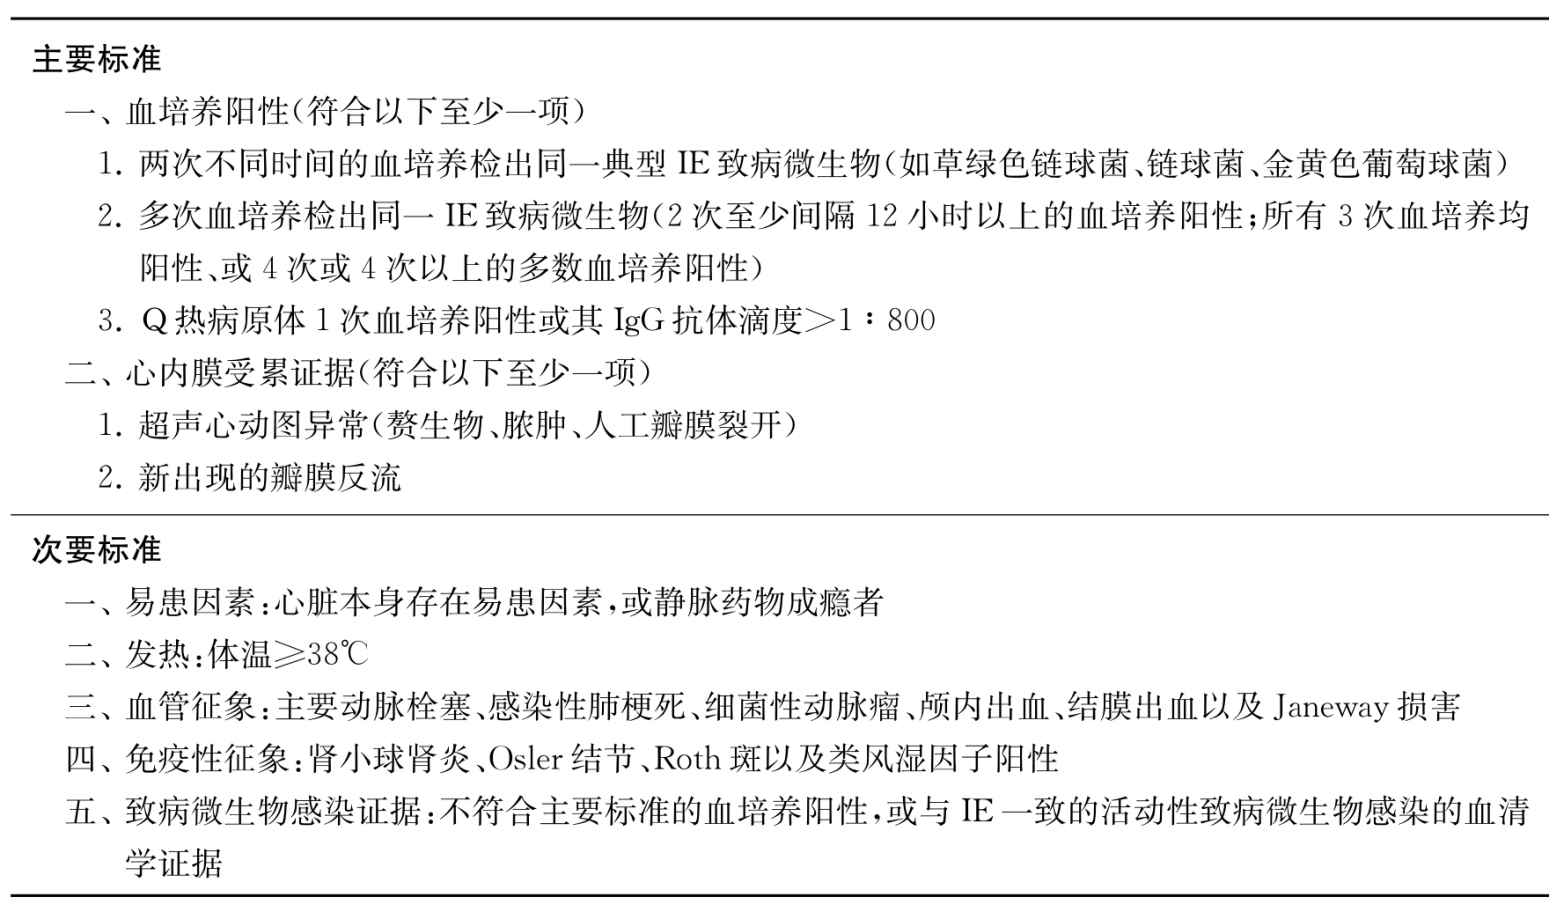
\includegraphics[width=5.91667in,height=3.44792in]{./images/Image00006.jpg}
\end{table}

\paragraph{三、急性肾盂肾炎}

本病多见于女性,尤其是生育年龄的妇女,而糖尿病患者及使用导尿管等装置的老年患者亦不少见。当患者有急起畏寒、发热,伴有腰痛、尿频、尿急、尿痛时,应考虑急性肾盂肾炎的可能。若尿常规检查证实有脓尿,则诊断大致可以成立。病原学的诊断有待细菌培养证实。若仅有高热而尿路症状不明显者,应与各种发热性疾病相鉴别。腹痛、腰痛明显者应与急性胆囊炎、阑尾炎、盆腔炎、肾周围脓肿等鉴别。一般经多次尿液检查即能诊断。B超或CT检查有助于胆囊炎和肾周脓肿的诊断。

\paragraph{四、急性胆道感染}

急性发热者伴有上腹绞痛时,应考虑急性胆道感染的可能,通过进一步检查诊断一般不困难(参见第78.1节)。老年患者由于疼痛的敏感性降低,可无胆绞痛的主诉,但胆囊区仍可有明显的压痛。本病应与急性病毒性肝炎、急性胰腺炎、左下肺炎、急性肾盂肾炎等疾病相鉴别。血清转氨酶及病毒性肝炎系列标志物、血和尿淀粉酶、X线胸片和尿液检查则有利于各自的诊断。B超、CT检查可发现胆系结石和梗阻。

\paragraph{五、细菌性肝脓肿}

寒战、高热、肝区痛或右上腹痛,体检肝大并有压痛或(及)肝区叩击痛,血象白细胞总数及中性粒细胞增加,应考虑本病。B超有助诊断,必要时在B超引导下行肝穿刺抽出脓液可确立诊断。阿米巴肝脓肿临床上与细菌性肝脓肿相似,但阿米巴肝脓肿起病较慢、病程较长、慢性消耗表现较常见,而高热及白细胞增多则较不明显,部分病例有痢疾史或证实有阿米巴肠病。B超引导下肝脓肿穿刺,典型阿米巴肝脓肿脓液为巧克力样,在抽脓最后部分近脓腔壁的脓液有可能找到滋养体。近年,无论是细菌性肝脓肿还是阿米巴肝脓肿临床表现不典型病例增多,常发生漏诊,应提高警惕。肝脓肿还要与肝癌(特别是肝癌中心坏死液化合并感染)、肝囊肿或肝包囊虫病合并感染、右膈下脓肿等疾病鉴别(参见第106.2节及第106.3节)。

\paragraph{六、其他急性局灶性细菌感染}

此类疾病的共同特点是高热、畏寒或寒战,周围血象白细胞和中性粒细胞增多,并有局部症状和体征。

\subparagraph{(一)膈下脓肿}

通常并发于腹腔化脓性感染或腹腔手术后,尤其是急性阑尾炎、胃及十二指肠穿孔、胆囊切除术、脾切除术后等。肝脓肿亦可直接向右膈下组织蔓延。若有上述情况,患者又出现寒战、高热、白细胞总数和中性粒细胞增高,又未能找到其他感染灶时,应想到此病的可能。膈下脓肿以右侧多见,患者自觉患侧上腹部有显著搏动性疼痛,以深呼吸或体位转动时加重,患侧下胸部常有局部皮肤水肿并有压痛及叩击痛,听诊呼吸音减弱或消失。站立位X线检查可发现患侧膈肌上升活动受限,反应性胸膜炎,患侧膈下可见液平面或气泡。B超或CT检查可早期明确诊断。

\subparagraph{(二)肾周围炎或肾周脓肿}

患者常以畏寒、发热或寒战高热开始,伴有患侧肾区疼痛,并向同侧下腹及大腿内侧放射,脊肋角显著压痛及叩击痛。当此病早期未出现肾周围局部体征时易误诊为全身感染或急性肾盂肾炎,及时进行B超或CT检查可明确诊断。

\subparagraph{(三)其他局灶性感染}

化脓性中耳炎、化脓性扁桃体炎、化脓性关节炎、化脓性骨髓炎以及其他各部位的浅部化脓性感染(如疖、皮下急性蜂窝织炎等)或深部化脓性感染(如臀肌脓肿、脑脓肿等)均可引起急性高热,局灶性症状和体征可提示诊断。

\paragraph{七、败血症}

败血症(septicemia)是指病原菌及其毒素侵入血流所引起的临床综合征,是一种严重的血流感染。尽管目前对败血症的定义仍有争议,但疾病国际分类(ICD)仍采用败血症这一病名。当患者有原发感染灶,出现全身性脓毒症症状,并有多发性迁徙性脓肿时提示败血症。值得注意的是有时原发的感染病灶可能很轻微或已愈合。因此,临床上遇到不明原因的急性高热,伴有畏寒或寒战、出汗,全身中毒症状重,白细胞总数和中性粒细胞明显增高,而无特殊症状、体征及流行病学病史提示急性传染病时,应考虑败血症的可能。医院内感染败血症绝大多数见于有严重基础疾病如各种血液病、肝及肾衰竭、晚期恶性肿瘤,或医源性感染如各种导管的长期置留、透析疗法等,如患者出现不明原因发热或(及)病情恶化时应注意败血症的可能。阳性血培养是诊断败血症的重要依据,反复多次做血培养可获得较高的阳性率。

根据我国近年对败血症病原学分析的报道,我国败血症的病原体以金黄色葡萄球菌、大肠杆菌和其他肠道阴性杆菌为多见,但表皮葡萄球菌、铜绿假单胞菌及一些耐药菌败血症有增加趋势,厌氧菌及真菌败血症亦非罕见。不同病原菌所造成的败血症临床表现可有一定差异,兹分述如下:

\subparagraph{(一)需氧革兰氏阳性球菌败血症}

\hypertarget{text00014.htmlux5cux23CHP2-5-1-2-7-1-1}{}
1.金黄色葡萄球菌败血症

此病较常见,国内对各地共1000余例次败血症的病原学分析表明,金黄色葡萄球菌败血症所占比例高达20\%~30\%。临床急起发病,常先有畏寒或寒战,继而高热、头痛与出汗,多伴有恶心呕吐、腹泻、全身肌肉及关节疼痛,皮疹形态多样化,可有瘀点、荨麻疹、猩红热样皮疹及脓疱疹等。迁徙性化脓病灶是本病的特点,对病因诊断有重要意义。迁徙性病灶以四肢和躯干的多发性软组织脓肿、多发性肺脓肿、脓胸、肝脓肿、化脓性脑膜炎、骨髓炎等多见。本病并发心内膜炎者可高达8\%。临床若遇发热持续不退,体检发现有心脏病理杂音的出现,伴有进行性贫血、反复出现皮肤瘀点、内脏血管栓塞、血培养持续阳性,应考虑心内膜炎的存在,及时做超声心动图有助确诊。

金黄色葡萄球菌败血症的诊断一般不难,当存在原发性皮肤化脓性病灶或导管插管处红肿热痛,出现寒战、高热等中毒症状时,首先应考虑本病的可能。若同时伴有皮疹与迁徙病灶,则可能性更大。但临床上部分患者急起发热,病史不清,会造或诊断困难。如当胸片发现多发性迁徙肺脓肿者,此时易误诊为肺炎;胸片有片状模糊阴影者,易误诊为肺结核;少数患者白细胞计数较低,发热呈稽留热时,可误诊为伤寒。提高对本病的警惕和认识。早期多次血培养有助于及早做出诊断。

\hypertarget{text00014.htmlux5cux23CHP2-5-1-2-7-1-2}{}
2.表皮葡萄球菌败血症

近年来本病逐渐增多,目前约占败血症总数的10\%~15\%,且70\%为医院内感染。常见于体内异物留置或植入者(如静脉导管、人工关节、人工瓣膜、起搏器等)。由于表皮葡萄球菌为正常皮肤表面的细菌,血培养假阳性率高,因此,血培养阳性难以鉴别是否为污染所致。然而当患者发热不退,体内留有异物(如静脉导管)处局部皮肤红肿、压痛,或人工瓣膜患者出现新的杂音或多发性血栓形成等,都是感染的有力证据。另外,双份(身体左右侧静脉)血培养同时阳性意义更大。

\hypertarget{text00014.htmlux5cux23CHP2-5-1-2-7-1-3}{}
3.肠球菌败血症

本病发病率近年未有明显增多的趋势,77\%为医院内感染,占院内感染败血症的10\%左右。病原菌常来源于泌尿生殖道,亦易发生于消化道肿瘤及腹腔感染的患者,因此,对有上述病史的急性发热患者,尤其是院内感染,要考虑本病的可能。由于本病对多种抗菌药物耐药,故病情多危重。

\subparagraph{(二)需氧革兰氏阴性杆菌败血症}

约占败血症总数的40\%左右,其中,最常见为大肠杆菌败血症,其次为肺炎克雷伯杆菌、铜绿假单胞菌和其他肠杆菌败血症。病原菌常从泌尿生殖道、肠道(尤其是下消化道)或胆道入侵,多见于一般体质较差,伴有各种影响机体免疫功能的原发病。热型不一,以弛张热多见,少数患者可有体温不升、双峰热。40\%患者可发生休克,休克的特点是出现早且持续时间较长,严重患者可出现多脏器功能损害。多数患者白细胞增高,少数患者正常或减少但常有中性粒细胞左移现象。本病与金黄色葡萄球菌败血症在临床上虽然很相似,但原发灶不同,早期出现休克以及迁徙病灶较少见,有临床鉴别价值。

铜绿假单胞菌败血症通常继发于重度烧伤、白血病、淋巴瘤、各种恶性实体瘤以及气管切开、静脉导管、导尿等。临床表现较一般革兰氏阳性杆菌败血症凶险,可有较特征性中心坏死性皮疹。患者淡绿色尿(绿球蛋白)可作为铜绿假单胞菌败血症的诊断佐证。

\subparagraph{(三)细菌L型败血症}

细菌在体内多种因素影响下失去细胞壁变为L型,临床上常在应用抗生素后产生。细菌转变为L型后临床表现与原菌感染不同,其常见临床表现为发热波动难以控制,多呈弛张热(占80\%)。胸片示间质性肺炎但呼吸道症状轻微,尤其是感染性发热应用抗生素后一度有效,以后发热起伏波动,白细胞总数不高而有核左移和中毒颗粒者。临床上L型细菌以金黄色葡萄球菌多见,因此,在无法确定其类型的情况下,可选择对L型金葡菌有效的抗生素进行试验性治疗。多次高渗及等渗双份血培养均培养出L型细菌可助确诊。

\subparagraph{(四)厌氧菌败血症}

厌氧菌多从肠道肿瘤、发炎的憩室、女性生殖道、压疮、感染的胆道等处入侵血流,常发生于有严重基础病免疫功能低下的患者。厌氧菌多与需氧菌同时混合感染。对有上述情况,敏感抗生素治疗效果不佳甚至恶化的败血症患者,应考虑厌氧菌混合感染的可能,应加做厌氧菌特殊培养以助诊断。病变组织有脏而臭的分泌物、含气体、有假膜形成是诊断的佐证。

\subparagraph{(五)真菌败血症}

主要以念珠菌感染为主,近年来发病率明显增高,绝大部分为机体抵抗力低下的医院内感染,常见于长期接受广谱抗生素、糖皮质激素、免疫抑制剂或肿瘤化疗患者。因此,对具有上述易感因素,持续高热,经足量高效抗生素治疗96小时无效,尤其存在真菌感染灶(如口腔黏膜、皮肤)者应警惕本病的可能。血培养发现真菌可确诊,但阳性率不足50\%,且培养费时较长。因此,对高度怀疑本病者,选择广谱的抗真菌药物治疗症状改善,体温下降至正常者,亦为有力的佐证。

\paragraph{八、结核病}

发热为结核病最常见的全身性毒性症状,多数为长期低热,但当病灶急剧进展扩散时则可出现高热,呈稽留热或弛张热热型,可伴有畏寒,但很少寒战。临床上属此类型者有急性粟粒型结核,某些肺外结核如网状内皮系统结核(无反应结核病)、结核性脑膜炎、浸润型肺结核。

\subparagraph{(一)急性粟粒型结核(急性血行播散型肺结核)}

急性粟粒型结核来源于自体结核病灶,当机体免疫功能低下时加重和恶化,并从血流播散。本病发病急骤,持续高热为早期或突出症状,中毒症状严重,有时伴有乏力、畏寒等非特异症状。由于临床上肺部粟粒型结核多见,患者常伴有咳嗽、咳痰、气短等呼吸道症状。病程中可伴有轻度肝脾大。周围血象中多数有白细胞减少,少数有全血细胞减少。亦有少数病例白细胞明显增高呈类白血病反应。本病早期胸部X线表现不明显或阴性时,易误诊为伤寒、败血症或恶性血液病。但本病患者常有呼吸道症状如咳嗽、气促等症状,且血象无相对的淋巴细胞增多,肥达反应阴性,多次血培养伤寒杆菌阴性可与伤寒鉴别。反复多次血培养无致病菌生长,高效广谱抗生素治疗无效,可与败血症鉴别。全血细胞减少又伴有肝脾大者,易与白细胞不增高的急性白血病或恶性组织细胞病混淆。本病在发病第一、二周内,由于病变太小,在胸片上不易发现病灶。因此,对怀疑本病者,若一次胸片阴性,应定期复查或行胸部高分辨CT检查,可发现典型的两侧肺野内大小相等、从肺尖到肺底均匀一致的粟粒状致密影。结核菌素试验阳性对诊断有参考价值,但阴性不能否定结核,特别是老年人或免疫功能低下的患者。此外,眼底检查近半数成人病例,可发现脉络膜上有灰白色或黄色圆形小结节,对本病的诊断极有帮助。

\subparagraph{(二)无反应结核}

属特殊类型结核病,见于免疫力严重低下患者,其特点为:①全身中毒症状较重,持续高热,故又称之为结核性败血症;②呼吸道症状出现较晚;③肝、脾、淋巴结肿大多见且早期出现;④可并发粒细胞缺乏甚至全血细胞减少,亦可呈类白血病反应;⑤合并肺门淋巴结或纵隔阴影增大者可高达72\%。本病临床上易与风湿性疾病、败血症、伤寒病、血液病和恶性淋巴瘤混淆,定期复查胸片或胸部CT,痰、淋巴结穿刺物涂片检出抗酸菌有助确诊。

\paragraph{九、伤寒与副伤寒}

\subparagraph{1.伤寒}

发热是伤寒的早期症状,有时为唯一症状,因此是未明原因发热经常要考虑的疾病之一。凡发热持续一周以上原因未明者,需注意伤寒的可能。传统观点认为具有诊断参考价值的临床表现有:①热型早期呈梯形上升,极期呈稽留热型持续,后期呈弛张型缓解,病程多为3~4周;②伤寒毒血状态,表现为表情淡漠,无欲面容;③相对缓脉与重脉;④发病一周左右胸前、腹上区分批出现少数玫瑰疹;⑤脾轻度肿大;⑥白细胞总数减少,相对淋巴细胞增多,嗜酸性粒细胞减少或消失。

近年来,我国伤寒的发病率已明显降低,其流行高峰亦已较为平坦,并发症已显著减少,且由于起病早期多已接受过抗菌药物治疗而致临床表现多不典型。因此,依靠流行病学资料和典型临床表现作出伤寒的临床诊断往往有困难,关键是要注意伤寒的可能。确诊主要靠病原学和血清学检查:①一周后肥达反应“O”抗体凝集效价≥1∶80,H抗体凝集效价≥1∶160,有诊断参考价值,病程中效价逐渐升高意义更大。但血清学诊断需密切结合临床,凝集效价持续阴性,不能作为否定伤寒的依据。②血、骨髓培养伤寒杆菌阳性是确诊的依据,尿、粪培养阳性可弥补血、骨髓培养的不足。

临床上对高度怀疑伤寒患者,亦可试用氟喹诺酮类、氯霉素、氨苄西林等进行诊断性治疗。用药后本病多在3~5日内体温逐渐下降,临床症状亦迅速好转。

\subparagraph{2.副伤寒}

流行病学特点与伤寒相同,但发病率远较伤寒低。副伤寒甲、乙临床表现难与伤寒鉴别,但副伤寒潜伏期较短,急性起病较多,早期胃肠炎症状较明显,热型不如伤寒典型。副伤寒丙可表现为轻型伤寒,急性胃肠炎或脓毒症。与伤寒相同,确诊有赖于病原学及血清学检查,但要注意副伤寒丙的血清凝集效价较低,少数患者可始终阴性。

\hypertarget{text00014.htmlux5cux23CHP2-5-1-2-10}{}
十、细菌性心包炎

结核性或化脓性心包炎:早期症状不典型,诊断较困难。因此,对不明原因的发热兼有心前区疼痛的患者,应想到本病的可能。体检发现心尖搏动弱,心脏扩大,心音遥远,应考虑本病。若心前区闻及心包摩擦音,可作出初步临床诊断。本病的心前区痛与急性心肌梗死疼痛类似,应注意鉴别。心电图、胸部X线有助诊断,心脏B超和心包穿刺可确诊。

\hypertarget{text00014.htmlux5cux23CHP2-5-1-2-11}{}
十一、兔热病

本病是土拉杆菌所致的急性传染病,属自然疫源性疾病,在我国见于西藏、青海、内蒙古、黑龙江及山东等地。主要传染源是野兔,其次是鼠类和羊。由直接接触,烹食未熟受染的野兔、松鼠及其他啮齿类动物,或被壁虱叮咬而受染。潜伏期一般为3~4日,起病大多急骤,高热伴寒战及毒血症状如头痛、肌肉酸痛,局部皮肤出现丘疹,继而化脓,坏死中心脱落而形成溃疡,边缘隆起有硬结感,伴有一定程度的疼痛。白细胞总数多正常,偶有轻度升高。土拉杆菌抗原皮内试验或荧光抗体试验有助于早期诊断。

兔热病分溃疡型和腺型、肺型、胃肠型、伤寒型或中毒型、眼腺型、咽腺型等不同类型。确诊有赖于血或病灶分泌物的细菌分离(特殊培养或动物接种)及阳性免疫反应。

本病应与鼠疫、炭疽、鼠咬热等的皮肤病灶和腺肿鉴别。尚应与各种肺炎、伤寒、结核、布鲁菌病、类鼻疽、组织胞浆菌病等相鉴别。

\hypertarget{text00014.htmlux5cux23CHP2-5-1-2-12}{}
十二、人感染猪链球菌病

猪链球菌病是由多种不同群的致病性链球菌引起的一种人畜共患传染性疾病,人感染猪链球菌并引起发病的情况比较少见,其传染源主要为猪链球菌感染的病猪和带菌猪,高危人群为屠宰、饲养生猪或加工、销售、运送猪肉类的人员,感染途径主要通过接触病死猪时致病菌经破损皮肤和黏膜侵入人体,或吃了未完全煮熟的病猪肉或内脏而感染,目前尚未发现人与人之间的传播。

人感染猪链球菌病潜伏期短,平均2~3天,可短至数小时,最长达7天。临床上可分为四种类型:普通型、休克型、脑膜炎型和混合型。起病急,临床表现为畏寒、发热、头痛、头昏等全身中毒症状。重症病例迅速进展为中毒性休克综合征,出现皮肤出血点、瘀点、瘀斑,血压下降,脉压差缩小;可表现出凝血功能障碍、肝、肾功能不全、急性呼吸窘迫综合征、软组织坏死,筋膜炎等。部分病例表现为脑膜炎,恶心、呕吐、昏迷,脑膜刺激征阳性,脑脊液呈化脓性改变。还有少数病例为混合型,即在中毒性休克综合征基础上,出现化脓性脑膜炎表现。部分病例在恢复期出现听力减弱、障碍。实验室检查外周血白细胞计数升高(严重患者发病初期白细胞可以降低或正常),中性粒细胞比例升高。诊断上结合疫情资料、流行病学调查资料和患者的发病情况、临床症状及早期病例的尸检报告可做出初步诊断;进一步的确诊有赖于实验室病原学诊断。

\protect\hypertarget{text00015.html}{}{}

\subsubsection{1.1.3 钩端螺旋体病}

鼠和猪是本病的主要传染源,其带有钩端螺旋体的尿可以污染各种水源,人与污染的水源接触,钩端螺旋体通过暴露部位的皮肤进入人体而造成感染。全国各地均有本病报道,但以南方各省多见。本病具有如下流行病学特点:①疫水接触史,患者在起病3~20天内到过鼠类出没或猪尿污染的污水沟、稻田,皮肤曾与污水接触。散发病例,因很多场所被污染,有时无明确接触史而常被误诊。②主要流行于夏秋收割季节,有时可在洪水过后造成流行。③患者多为青壮年农民、饲养员,外地进入疫区者亦易患病。本病临床表现复杂,临床表现轻重不一,轻者似感冒,仅表现为轻度发热。典型的临床特点为:早期有高热,全身酸痛,结膜充血,腓肠肌压痛及浅表淋巴结肿大等类似败血症的表现。中期为肝、肾、肺等多器官损害与功能紊乱。

本病可分为流感伤寒型、肺出血型、黄疸出血型、肾衰竭型和脑膜炎型。流感伤寒型多数以全身症状为特征,起病急骤,畏寒发热,头痛、全身肌痛并有鼻塞、咽痛、咳嗽等,而无黄疸和中枢神经系统症状,肺亦无明显病变,易误诊为流行性感冒、上呼吸道感染。但本病患者往往同时或随之出现肝、肾功能损害,半数有皮肤黏膜出血,不支持流感和上呼吸道感染。仔细调查流行病史有助于鉴别诊断。肺出血型应与肺结核、支气管扩张、肺肿瘤鉴别。通过胸部X线或CT等检查加以区别。黄疸型易误诊为黄疸型肝炎,但后者以纳差为主,无眼结合膜充血和腓肠肌压痛,ALT、AST明显升高,而CPK不高,病毒性肝炎系列标志物和流行病学史可资鉴别。肾衰竭型与流行性出血热临床表现有相似之处,但后者通常有酒醉貌,无腓肠肌压痛,流行性出血热特异性抗体和病毒抗原检查有助于两者鉴别。脑膜脑炎型的钩端螺旋体病与乙脑都在夏秋季流行,但后者无全身酸痛、结膜充血和腓肠肌压痛,且乙脑抽搐、昏迷等脑部症状较钩端螺旋体病明显,尿常规、肝功能多正常。

对于钩端螺旋体病的病原学诊断,应用暗视野显微镜可直接检查患者血、尿及脑脊液等标本中的钩端螺旋体。病原体分离可用体液培养或动物接种技术。血清补体结合试验和凝集溶解试验自病程第一周末开始升高,在第三、四周达高峰,间隔两周双份血清,效价增高4倍以上有诊断价值。酶联免疫吸附试验比凝溶试验阳性出现更早和更灵敏,有早期诊断价值。

\protect\hypertarget{text00016.html}{}{}

\subsubsection{1.1.4 立克次体感染}

\paragraph{一、斑疹伤寒}

流行性斑疹伤寒在我国已基本得到控制;地方性斑疹伤寒由鼠蚤传播,属自然疫源性疾病,国内以河南、河北、山东和辽宁等地报道的病例较多,以夏秋收割季节发生较多。本病以高热、剧烈头痛、全身肌痛起病,眼结膜充血,可有中枢神经系统临床表现。早期病例需与流感、流行性出血热、钩端螺旋体病、伤寒、恙虫病、流行性脑脊膜炎、大叶性肺炎等疾病鉴别。一旦典型皮疹出现(一般在4~6天内),则病象相当明显,参见第2.1节。

\paragraph{二、恙虫病}

恙虫病流行于夏秋季,患者在疫区的田野或草地上工作、卧息时,可因被受染恙螨叮咬而感染。流行季节有不明原因急性发热患者,要警惕本病的可能。须追查流行病学史与细致搜寻焦痂,参见第2.1节。

\protect\hypertarget{text00017.html}{}{}

\subsubsection{1.1.5 寄生虫感染}

\paragraph{一、疟 疾}

间日疟和三日疟具有间歇性、规律性、发作性寒战、高热和大汗,伴有贫血和肝脾大等典型的临床表现,诊断不难。而恶性疟疾的临床症状较复杂而多样化,发热前寒战较少,热型多不规则,热后较少出汗。伴头痛、肌痛、纳差等症状,常有恶心、呕吐、腹泻等消化道症状。高热患者常有剧烈头痛,并出现谵妄、抽搐和昏迷,脑膜刺激征明显(脑型疟疾),易误诊为乙型脑炎。部分恶性疟患者有相对缓脉,加之有脾大和白细胞减少,易与伤寒相混淆。因此,在到过疟疾流行地区后出现不明原因的发热,应警惕疟疾的可能。疟原虫的发现是诊断疟疾的主要依据,一次血片检查阴性不能否定,应在发作过程中反复检验。在发热前的畏寒期采血作厚滴片检查,可提高阳性率。血片阴性时可作骨髓涂片检查,其阳性率较血片为高。氯喹或奎宁对疟疾治疗有特效,一般用药后1~2天体温下降,症状基本控制,对高度疑似的病例可用常规剂量作诊断性治疗。

\paragraph{二、阿米巴肝脓肿}

见前述及参见第106.3节。

\paragraph{三、急性血吸虫病}

本病多发生于夏秋季,有严格的地区性,多见于初次接触疫水感染者,但慢性血吸虫患者在再次大量感染后亦可表现为急性感染。平均潜伏期40日左右,其间可出现疫水接触处皮肤发痒,红色小丘疹约1~2日消失。急性患者都有发热,发热的高低、热型、热程与感染轻重因个体反应不同而异。可高热持续不退,伴精神萎靡、意识淡漠,重听、腹胀、可有相对缓脉而误诊为伤寒,但白细胞总数增高及分类中嗜酸性粒细胞增多(一般占20\%~40\%),据此可与伤寒鉴别。急性血吸虫患者有肝大,伴不同程度压痛,以左叶为著,与肝脓肿相似,但B超、CT发现占位病变可资区别。血吸虫卵所造成的异位肺损害,除有呼吸道症状外,胸片常示两肺中下野、大小略不等粟粒点状影应与粟粒型结核相鉴别。肠道症状表现为腹泻、腹痛、黏液血便,部分患者可出现腹膜刺激征,腹部饱满,有柔软感和压痛,类似结核性腹膜炎。凡夏秋季接触疫水,病初出现尾蚴皮炎,具有发热、肝大伴压痛、腹痛腹泻,而血中嗜酸性粒细胞明显增高者,需考虑急性血吸虫病的诊断。但不典型和重笃病例可不出现嗜酸性粒细胞增高或反而减少,据此,亦不能完全否定急性血吸虫病的可能。下述检查有助于确立急性血吸虫病的诊断:

1.血清免疫学检查

(1)抗体检测:常用检测方法有环卵沉淀试验(COPT)、间接血凝试验(IHA)、酶联免疫吸附试验(ELISA)等。COPT法目前仍为疫区广泛应用。近年来建立的简便快速的ELISA方法、敏感度达90\%以上,且敏感性和重现性好。但应注意抗体检测法不能区别既往感染与现症患者。

(2)抗原检测:可证实活动性感染。单克隆抗体斑点酶联法检测循环抗原敏感性和特异均较高,其临床应用尚在进一步研究中。

2.目前采用尼龙袋新鲜粪便集卵孵化法,提高了阳性率,为主要的检查方法。但一次阴性不能轻易除外本病,宜反复多次进行,以获得病原学的诊断。

3.直肠黏膜活组织检查,可提高检出虫卵的阳性率。

\paragraph{四、旋毛虫病}

猪为人体旋毛虫感染的主要传染源。本病发病前1~2周有生食或半生食含旋毛虫幼虫包囊的猪肉史,初期主要为肠炎症状,如腹痛、腹泻和稀水便;急性期发热多在38~40℃之间,热型多为弛张热,也可呈不规则热,伴有肌肉疼痛和水肿、皮肤斑丘疹或猩红热皮疹等,血象白细胞和嗜酸性粒细胞增高,确诊有赖于胸大肌或腓肠肌肌肉活检找到梭形包囊和幼虫和(或)免疫学检查等。

\protect\hypertarget{text00018.html}{}{}

\subsubsection{附:丝虫病}

丝虫病系由丝虫寄生于淋巴组织、皮下组织或浆膜腔所致的传染病。淋巴丝虫病是由班氏、马来或帝汶丝虫寄生于淋巴组织所致的传染病。我国除山东、台湾为单纯班氏丝虫流行外,其余地区均有两种丝虫病流行。在丝虫病疫区,患者有发热、淋巴管(结)炎、阴囊内器官与组织炎症或象皮肿,血中嗜酸性粒细胞增多,须考虑丝虫病。

班氏丝虫寄生于深部或浅表淋巴结、淋巴管中,尤以腹腔、盆腔、腹膜后组织、肾盂、附睾、精索等部位为多。因此,除有肢体淋巴管炎外,尤以阴囊内器官与组织的炎症病变为多见,阻塞胸导管或乳糜池可致乳糜尿。马来丝虫主要寄生于人体四肢浅部淋巴系统,尤以下肢多见,因此,肢体淋巴管炎和象皮肿较明显,无乳糜尿及外生殖器局部病征,巨型象皮肿亦较少见。帝汶丝虫病主要表现为腹股沟、股及沿大隐静脉和其分支的淋巴管炎、淋巴结炎及膝部以下象皮肿。

丝虫病发热的特点是往往呈不规则的周期性发作,通常伴淋巴管、淋巴结炎。少数病例的淋巴管炎位于腹内深处,可无浅表病理体征。有些病例如阴囊内器官与组织炎症,在急性发作期疼痛可先从下腹部开始,或向腹部放射,故易误诊为阑尾炎或其他急腹症,但体检时腹部体征阴性而阴囊内有器官与组织炎症存在,可资鉴别。此外,精索与附睾炎要与附睾结核鉴别,后者结节在附睾内,常粘连在一起,不痛,少有反复发作。

病原学检查发现微丝蚴为确诊的直接证据。于晚间熟睡时采周围血作成厚涂片,每夜连续2~3次,检出率可达90\%以上。有实验条件者,采用间接荧光抗体或酶联免疫吸附试验可检测丝虫特异抗体。对疑似病例,服用乙胺嗪后肢体淋巴管或阴囊内出现新结节,或阴囊内原有病变增大、疼痛加剧,对丝虫病的诊断有一定的辅助诊断价值。

1994年,全国864个流行县、市(含班氏和马来丝虫病)全部达到基本消灭丝虫病标准,实现全国基本消灭丝虫病的目标。

\protect\hypertarget{text00019.html}{}{}

\subsection{1.2 非感染性急性发热疾病}

\subsubsection{一、风湿热}

风湿热是一种常见的反复发作的急性或慢性全身性结缔组织炎症,主要累及心肌、关节、中枢神经系统、皮肤和皮下组织。本病最常见于5~15岁的儿童和青少年,多数患者发病前1~5周先有咽炎或扁桃体炎等上呼吸道感染史。

风湿热患者多有低热,中等度热,亦可呈现高热。部分病例没有明显关节痛或关节炎的症状、以发热为主要临床表现,诊断有时困难。

迄今风湿热尚无特异性的诊断方法,主要依靠临床表现与动态观察,辅以实验室检查。临床上沿用修订的Jones诊断标准,认为具有下述2项主要表现或1项主要表现加2项次要表现,并先前有链球菌感染的证据,可诊断风湿热。

主要表现:①心脏炎:为临床上最重要的表现,其特征有:a.心肌炎,最早的临床表现为二尖瓣和主动脉瓣的器质性杂音。心尖区第一心音常减弱,常可闻及奔马律;b.心动过速,常>100次/分,与体温不成比例;c.心脏扩大;d.心律失常及心电图异常,常见为房室传导阻滞、期前收缩和心电图PR间期延长;e.心力衰竭,往往由急性心肌炎所致,尤其多见于年龄较小的患者;f.心包炎,出现于风湿热活动期,为严重心脏炎的表现之一。②多发性关节炎。③舞蹈病。④环形红斑。⑤皮下结节。

次要表现:①关节痛;②发热;③急性反应物改变(血沉降率增快,C反应蛋白增高);④心电图PR间期延长;⑤既往风湿热史和现患风心病。

有链球菌感染证据:①近期患过猩红热;②咽喉拭子培养或快速链球菌抗原试验阳性;③链球菌抗体效价升高。

在上述5项主要表现中,心脏炎和多发性关节炎的诊断意义最大。但亦非特异性。风湿热累及心肌时,表现为与发热不相称的心动过速和心电图异常改变,常有诊断参考价值。但由于也非特异性,亦需在鉴别的基础上考虑诊断。由于多关节炎的疾病种类繁多,多关节痛在几乎所有发热性疾病中经常可见,临床工作中,易将有类似表现的骨、关节和其他风湿性疾病如系统性红斑狼疮等误诊为风湿性关节炎,应予以重视。另一方面,约有1/4风湿热患者无多关节炎症状,甚至无关节痛,据此就不考虑风湿热的诊断,是另外一种错误倾向,应有所认识。风湿性心包炎的心包摩擦音,由于持续时间短暂,易被忽略而漏诊。主要表现中的后3项,发生率甚低,在诊断中起作用少。但少数患者尤其是儿童出现舞蹈病,结合某项其他表现,则有可靠的诊断价值。

上述的实验室检查是诊断风湿热的参考条件,但必须结合临床资料综合分析。抗“O”滴度>500U,认为有参考诊断价值,但不能作为确诊的依据。因为其阳性率仅有70\%~80\%,且仅表示新近有过链球菌感染,ESR在合并严重的心力衰竭时可以正常。部分风湿热患者白细胞计数增高。心电图有P-R间期延长、不完全性或完全性房室传导阻滞,多源性或多发性期前收缩、二联律、阵发性心动过速或房颤,QT间期延长有较大的参考诊断价值。但其心电图改变亦非经常出现,需定期反复复查才能发现异常,且上述心电图改变亦非风湿热特有。

1992年美国心脏病学会对Jones标准又进行了修订:该标准保留了Jones原5项主要表现,减去1项次要表现(既往风湿热史和现患风心病),并指出有下列3种情况时可不必严格执行该标准,即:①舞蹈病者;②隐匿发病或缓慢发展的心脏炎;③有风湿热病史或现患风心病,当再次感染A族链球菌有风湿热复发的高度危险性者。

患有风湿性心脏病患者有发热时,须考虑风湿性心内膜炎与亚急性细菌性心内膜炎两者的鉴别。后者多见于原有心瓣膜病,有进行性贫血、脾大、瘀点、瘀斑,可有脑、肾、肺等不同部位的栓塞症状。反复血培养阳性,超声心动图在瓣膜上发现赘生物可资鉴别。对已证实合并亚急性细菌性心内膜炎的风湿性心脏病患者,经足量抗生素治疗症状无改善或一度改善后又恶化,下列表现提示有风湿活动:①上呼吸道感染出现心悸、气促、病程超过半月以上者;②原因不明的难于纠正的进行性心力衰竭或急性肺水肿;③ESR增快,心力衰竭时ESR正常,心衰好转后ESR反而增快;④洋地黄治疗效果不好或耐受量降低易出现中毒症状;⑤不明原因的心律失常;⑥原有器质性心脏杂音性质的改变;⑦出现心脏以外的风湿性病变如风湿性脑病、脉管炎、关节炎、环形红斑等。此时做抗心肌抗体检测,心脏炎者阳性率达70\%,特异性高,抗A组链球菌胞壁多糖抗体(ASP)明显升高,阳性率达80\%以上,有助于判断风湿活动和其他心脏病鉴别。

如发热患者伴多关节炎、ESR增快,也可见于诸多结缔组织病、结核性关节炎或结核感染反应性关节炎、各种败血症引起的感染性关节炎或关节痛。此外,风湿热还要与SLE、成人Still病、莱姆病(Lyme病)、急性白血病,链球菌感染后状态等鉴别。

近年来风湿热、风湿性关节炎已明显减少,典型病例已不多见。但轻症、不典型病例仍可见到,给诊断带来一定的困难。

\subsubsection{二、系统性红斑狼疮}

部分系统性红斑狼疮早期可仅以发热为突出症状,其他系统受累的症状和体征可以不明显,诊断有一定困难。未明原因的无菌性急性发热,尤其是生育年龄的妇女,应考虑到本病的可能,并作进一步相关检查,参见第5.3节。

\subsubsection{三、急性白血病}

临床上凡患者急起发热兼有进行性贫血及(或)出血倾向,须考虑急性白血病的可能性。典型的急性白血病有持续发热、出汗、衰弱、出血倾向、进行性贫血、胸骨压痛,肝、脾及(或)淋巴结肿大,周围血细胞高度增多(也可正常或减少),以原始白细胞占优势,血培养阴性等表现。根据血象与骨髓象通常不难作出诊断。有的病例须与类白血病反应相区别,参见第5.2节。

\subsubsection{四、热射病}

热射病(包括日射病)亦称中暑性高热。表现为高热(>40℃)和神志障碍。本病基本上发生于高温季节,临床上可分为两种类型:劳力性和非劳力性(或典型性)。前者主要是在高温环境下内源性产热过多;后者主要在高温环境下体温调节障碍引起散热减少。

\paragraph{1.劳力性}

其特点是在高温环境和无风天气下进行体力劳动或剧烈运动时发病,多见于平素健康的年轻人。早期有头痛、乏力、恶心、口渴、心烦、少汗或多汗等非特异症状,继而急骤发病,体温急剧升高至40℃以上,皮肤灼热干燥,心率可达160~180次/分。脉压增大,可发生谵妄、抽搐、昏迷、出现病理神经反射。此种患者可发生横纹肌溶解和多器官功能衰竭,甚至死亡。

\paragraph{2.非劳力性}

在高温环境下,多见于居住拥挤和通风不良的城市老年人、产妇、体弱或患慢性病者。表现为皮肤干热、发红、无汗。病初可有各种行为异常和癫痫发作,继而可发生谵妄、昏迷、瞳孔对称缩小,终末期散大,严重者可出现低血压、休克、心律失常及心力衰竭、肺水肿、脑水肿。

根据病史和体征,本病一般不难诊断。尤其患者有高温接触史,出现昏迷和体温过高时应考虑热射病的可能。在诊断本病前应与脑炎、脑膜炎、脑型疟疾、脓毒病、脑血管意外、产褥热、甲状腺危象、抗胆碱能药物中毒及其他急性感染性疾病相鉴别。

\subsubsection{五、药物热}

药物热是机体对药物的一种超敏反应。常与特异性体质有关。患者往往先有感染,在给药后7~10天出现发热,多为低热或中等度发热,也可表现为高热。药物热大多数伴有药物皮疹或荨麻疹、肌肉关节痛,但有少数病例仅表现为发热,无皮疹及其他症状,一般情况好。药物热一般在停药后48小时内热退。再用该药,则在数小时内再次引起发热。药物热应与感染性疾病感染未能控制及风湿性疾病、肿瘤引起的发热相鉴别。

\subsubsection{六、恶性高热}

恶性高热是使用全身麻醉剂产生的严重并发症。麻醉剂以肌肉松弛剂和吸入性麻醉剂合用时发生率更高。家族性遗传性体质缺陷是内在的重要因素,其中以遗传性肌病更为重要。本病常在麻醉后立即发生,心律不齐是早期表现,常伴呼吸困难、发绀,常伴全身骨骼肌强直。高热或特高热是必有的主要症状,可高达40℃以上。高热期间血清肌酸磷酸激酶、丙氨酸基转移酶、乳酸脱氢酶增高,还可出现肌红蛋白血症,尿中出现肌红蛋白。常因心力衰竭、脑水肿、急性肾功能衰竭而死亡。诱发恶性高热的药物有琥珀酸胆碱、氟烷、乙醚、环丙烷、氯仿、甲氧氟烷、氯胺酮、氨氟醚等。

本病应与甲状腺功能亢进危象、嗜铬细胞瘤及恶性综合征等相区别。恶性综合征是抗精神病药物治疗特有而罕见的严重反应,主要表现为持续高热、肌肉僵硬、意识障碍及心血管症状等,可导致死亡。

\subsubsection{七、组织坏死性淋巴结炎}

组织坏死性淋巴结炎又称Kikuchi病,1972年由日本人首先报道,是一种主要累及淋巴结的良性、自限性、全身性疾病,误诊率较高,可达30\%~40\%。本病好发于青年女性,近年发病率有上升趋势,多累及颈部淋巴结,也可多部位先后出现淋巴结肿大,直径多在0.5~2.5cm;肿大淋巴结活动、无粘连,伴疼痛或压痛;发病前多有类感冒症状,体温38~39.8℃,抗生素治疗无效;实验室检查发现外周血白细胞计数在正常范围内或降低,血沉升高,PPD试验阴性。活检淋巴结破碎是特征之一。本病糖皮质激素有效是其特点,自然病程1~4个月。

\protect\hypertarget{text00020.html}{}{}

\subsection{1.3 急性“未明热”}

有少数急性发热患者未能查明原因,这些急性“未明热”以夏、秋二季为多见,且多见于年轻人。这些患者有急性感染的全身症状、体检及实验室检查无异常发现,病程通常在一周左右,预后良好。但是“未明热”仅为少数,有些病例由于检查未能周详及受设备条件或目前的认识所限,一时未能作出病因诊断,故诊断要慎重。必须除外引起急性发热的器质性疾病,首先要考虑病毒感染,其次为细菌感染如顿挫型伤寒、潜在的肺外结核、某些隐蔽的肿瘤等均要仔细排除。

\protect\hypertarget{text00021.html}{}{}

\section{2 急性发疹性发热}

在临床工作中,皮疹是常见的体征,据统计有100多种疾病发热伴有皮疹,常见有急性发疹性传染病、结缔组织病、变态反应性疾病、血液病等。一些原因不明的发热性疾病亦可发生皮疹,由于在不同疾病,皮疹可有不同形状,发疹时间及伴随症状也不相同。因此,可作为不同疾病鉴别诊断的一个重要体征(表\ref{tab2-3})。

\begin{table}[htbp]
\centering
\caption{急性发疹性发热性疾病的分类}
\label{tab2-3}
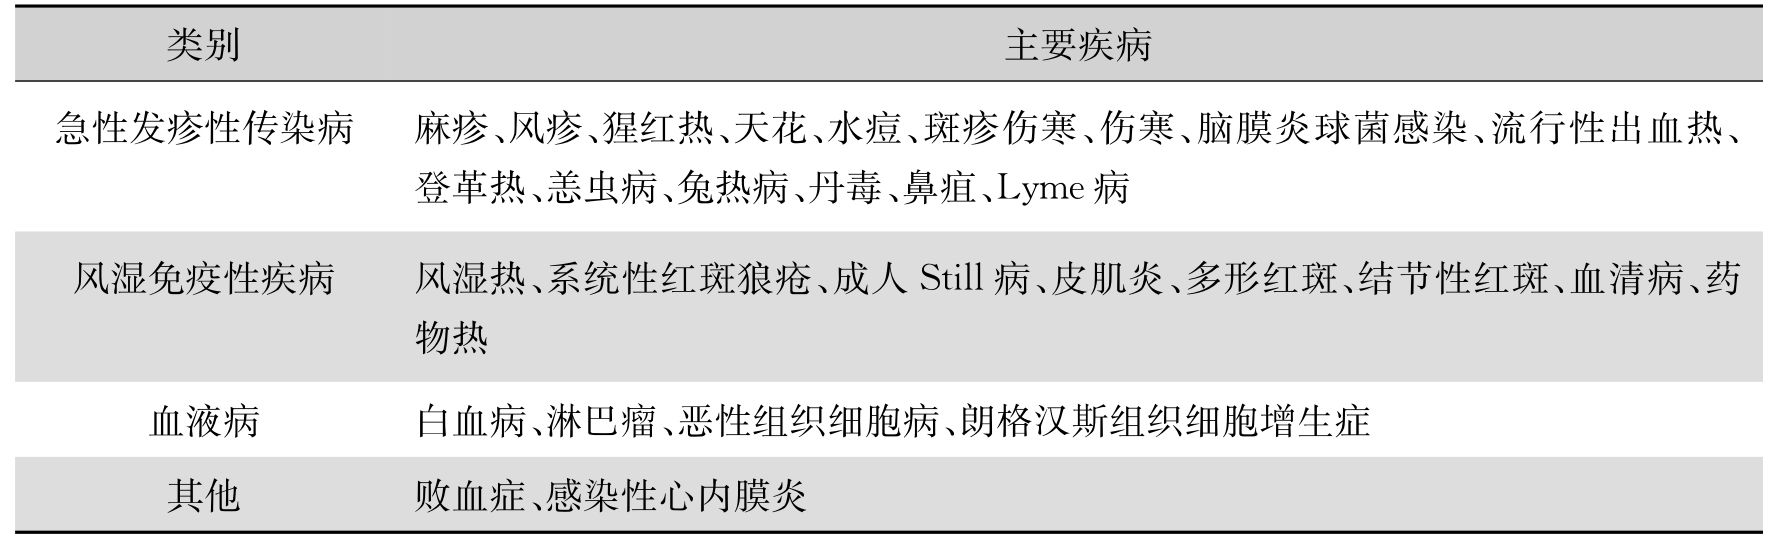
\includegraphics[width=5.9375in,height=1.84375in]{./images/Image00007.jpg}
\end{table}

\subsection{2.1 急性发疹性传染病}

急性发疹性传染病均有一定的潜伏期,掌握出疹的时间及其与发热的关系、出疹的部位及顺序、皮疹的性质及其相关体征、病程的经过,在鉴别诊断中有重要意义。

\subsubsection{一、麻 疹}

多在冬春二季流行,以儿童为多见。潜伏期为7~14天,发热3~5日出疹,主要症状有发热及上呼吸道卡他症状,同时有眼结膜充血、流泪、畏光日渐加重的表现,在发病第2~3日又可于双侧近臼齿颊黏膜处出现细砂样灰白色小点,绕以红晕,称麻疹黏膜斑,为本病早期特征。起病3~5日后,全身症状及上呼吸道症状加重,体温再度升高可达40℃,皮疹先于耳后发际出现,然后迅速发展到面部,自上而下蔓延直至手心足底;皮疹为淡红色、散在,然后密集呈鲜红色,持续约5日左右。皮疹出齐后按出疹顺序隐退、脱屑、色素沉着、整个病程10~14日。上述皮疹的临床表现,结合流行病史,血象白细胞计数正常或减少,80\%~90\%患者鼻咽、眼分泌物涂片染色镜检可发现脱落的上皮多核巨细胞、并可寻找到特异性麻疹抗原可诊断。从上述分泌物或血液白细胞中分离到麻疹病毒则可确定诊断。

在近期接受过免疫抑制剂或接种过疫苗者,全身症状轻、皮疹散在、不留色素,甚至可无皮疹和口腔黏膜斑。出血性皮疹多见于免疫力低下的重型患者。

成人麻疹的临床表现与儿童大致相同,但一般中毒症状较重,并发症也不少,且以呼吸道并发症多见。

麻疹需与风疹、猩红热、药疹等相区别。

\subsubsection{二、风 疹}

潜伏期较长为14~21天左右,主要发生于儿童,亦可见于青少年。临床症状较麻疹轻,发热仅1~2天,起病后即有皮疹出现,分布于颜面部,迅速波及躯干部,皮疹呈现玫瑰色斑丘疹,可融合成片。体温随皮疹的出现而上升,但较少超过39℃,通常2~3天内退热。其重要体征为伴有耳后、枕部甚至全身淋巴结肿大,无压痛。与麻疹的皮疹不同的是,皮疹的消退和发展同样迅速,疹退时体温亦下降,肿大的淋巴结亦逐渐恢复。皮疹消退后一般不留色素沉着,亦不脱屑。

风疹早期白细胞总数减少,淋巴细胞增多,并出现异形淋巴细胞,浆细胞增多,特异性风疹抗体IgM阳性有诊断意义。

风疹患者的皮疹形态介于麻疹与猩红热之间,因此,应着重对此三种常见的发热性出疹性疾病进行鉴别诊断。流行病学资料对鉴别诊断有重要帮助。

\subsubsection{三、传染性红斑}

本病病原为B19病毒,发病多见于儿童,少数亦可见于成人。潜伏期为4~12天,皮疹在第1~2天出现,最初为颊部水性红斑。后为全身斑丘疹,呈环形、网状,常有痒感,四肢亦可出现对称性斑丘疹,但罕见于手掌和足底。往往能同时出现发热、上呼吸道症状、肌痛和胃肠道症状。血清或咽拭子检测到特异性IgM抗体可确立诊断。本病需与药物疹、风疹和猩红热相鉴别。

\subsubsection{四、水 痘}

水痘是由于水痘带状疱疹病毒引起的急性传染病,多见于小儿,其潜伏期为10~24天。皮疹常于发病数小时或1~2天内分批出现,往往同时出现发热、头痛、咽痛、四肢酸痛和胃肠道症状。皮疹先见于躯干,逐渐延及面部,最后达四肢。皮疹呈向心性分布,以躯干为多,面部及四肢较少。皮疹发展快为本病的特征之一,开始为粉红色帽针头大的斑疹,数小时内变为丘疹;再经数小时变为水疱。短者这一过程仅6~8小时。水痘初呈清澈水珠状,以后稍混浊,壁薄易破,疱疹在24小时内开始皱缩、结痂。痂皮脱落后遗留浅瘢痕。水痘典型病例诊断不难,必要时可作血清学补体结合试验,出疹后1~4日即出现补体结合抗体阳性,可协助诊断。近年应用PCR方法检测鼻咽部分泌物VZVDNA,为敏感和快速的早期诊断手段。

水痘主要与轻症天花相鉴别,其鉴别要点如表\ref{tab2-4}。

\begin{table}[htbp]
\centering
\caption{水痘与天花的鉴别诊断}
\label{tab2-4}

\includegraphics[width=6.04167in,height=3.8125in]{./images/Image00008.jpg}
\end{table}

\subsubsection{五、登革热}

登革热为登革病毒引起,经蚊传播的急性传染病,多流行于夏秋季节。潜伏期2~15日。其临床特征为双相热、剧烈头痛、皮疹、肌肉骨关节剧烈酸痛、淋巴结肿大、白细胞和血小板减少、淋巴细胞相对增多。

本病多数起病急骤,常以畏寒发热开始,颜面及眼结膜显著充血,颈及上胸皮肤潮红,发热持续2~4天即退,皮疹常于发病后2~5天出现。初见于掌心、脚底或先发生于躯干及腹部。然后蔓延至全身。皮疹呈麻疹样,少数呈猩红热样,或介于两者之间,压之褪色。体温下降者此时又可再次上升(呈马鞍热)。皮疹于1~5日(平均3日)消失,体温同时下降。整个病程约5~7日。本病确诊有赖于病毒分离。目前国内用酶联免疫吸附试验检测特异性IgM抗体,对早期诊断有较大的意义。PCR方法检测登革热病毒RNA,具有快速、敏感性高、特异性强的优点。

\subsubsection{六、斑疹伤寒}

斑疹伤寒可分为流行性斑疹伤寒和地方性斑疹伤寒,两者临床特征相近似,但后者病情较轻,病程亦较短,皮疹很少呈出血性。

典型的斑疹伤寒,流行于冬春季节,其潜伏期为5~21天,常急骤起病,体温于第2~4天即达高峰(39~40℃),呈稽留高热型,伴有速脉(与体温升高程度呈正比)、头痛、周身肌肉痛、眼结膜及脸部充血。皮疹于病程第4~6日出现,为本病重要体征,见于80\%以上病例。初见于胸背、腋窝、上臂两侧,1日内迅速波及全身。而面部及下肢皮疹较少。但可出现于手心和足底,皮疹初为鲜红色,继而转为暗红或瘀点状。神经系统症状明显且出现早,头痛、呆滞、神志迟钝,加之患者有脾大,酷似伤寒。但本病一般无相对缓脉,血、粪培养阳性可资区别。部分流行性斑疹伤寒有腓肠肌压痛、肝大、黄疸和肾损害,少数伴有出血皮疹,在南方地区易与钩端螺旋体病混淆。但后者有疫水接触史,有全身出血倾向,皮肤出血而非呈斑丘疹状,白细胞增高,ESR增快,血清凝溶试验阳性可资鉴别。

流行性斑疹伤寒的诊断有赖于血清学检查:①外斐试验其凝集效价>1∶320,有参考诊断价值,因为非立克次体病变等也可出现阳性反应,但效价较低。复发型斑疹伤寒外斐试验往往阴性或效价<1∶160,故有鉴别诊断价值。②以提纯的普氏立克次体颗粒性抗原作补体结合试验,不仅具群特异性,且具种特异性,可区别流行性斑疹伤寒和地方性斑疹伤寒。③以可溶性抗原作立克次体凝集试验,特异性高,操作简便,可用于与其他群立克次体区别。且流行性斑疹伤寒的凝集抗体为IgM,复发型斑疹伤寒为IgG,两者可作鉴别。④分子生物学检查,用DNA探针或PCR方法检测普氏立克次体特异性DNA,具快速、特异、灵敏等优点,但作为诊断依据时,仍需结合临床表现和流行病学资料作出判断。

流行性斑疹伤寒与地方性斑疹伤寒的鉴别见表\ref{tab2-5}。

\begin{table}[htbp]
\centering
\caption{流行性斑疹伤寒与地方性斑疹伤寒的鉴别}
\label{tab2-5}

\includegraphics[width=5.94792in,height=1.67708in]{./images/Image00009.jpg}
\end{table}

斑疹伤寒还应与伤寒、回归热、流行性脑膜炎,流行性出血热、恙虫病、麻疹等鉴别。依据流行病学史及相关的实验室检查,一般可作出鉴别诊断,与伤寒的鉴别见表\ref{tab2-6}。

\begin{table}[htbp]
\centering
\caption{斑疹伤寒与伤寒的鉴别}
\label{tab2-6}
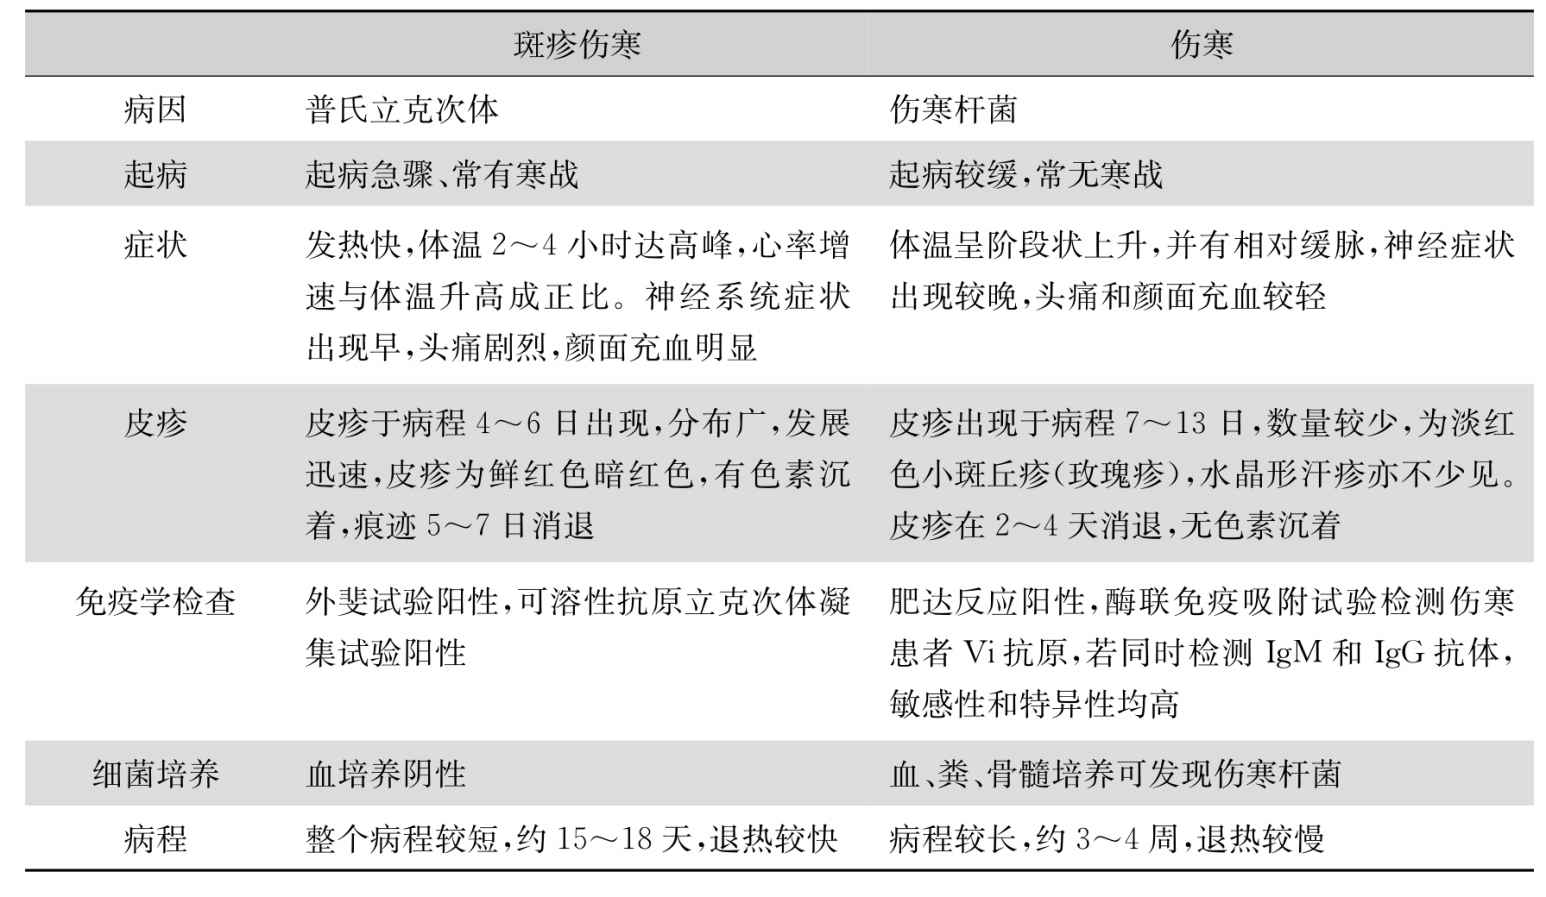
\includegraphics[width=5.95833in,height=3.45833in]{./images/Image00010.jpg}
\end{table}

\subsubsection{七、恙虫病}

恙虫病的潜伏期为5~20日,流行于夏秋季节,农民、与草地接触频繁的青少年及从事野外劳动者易得此病。起病多突然、体温迅速上升,达39~40℃,伴寒战、头痛、四肢酸痛、颜面潮红、结膜充血,类似斑疹伤寒的面容。严重者有谵妄、重听、腹胀、神志改变,部分患者可发生肠出血,易误诊为伤寒。焦痂和溃疡为本病的特殊体征,见于65\%~98\%患者。焦痂多见于腋窝、腹股沟、会阴、外生殖器、肛门等处。幼虫叮咬处出现红色丘疹,成水疱后破裂,中央坏死,结痂呈褐色或黑色,痂皮脱落后成小溃疡,边缘略隆起,底部为淡红色肉芽肿。因焦痂与溃疡无痒痛,发生于隐蔽部位,易被忽略。但仔细体检,往往可发现焦痂或溃疡,其附近的淋巴结肿大疼痛,有助于本病的诊断。

皮疹的发生率自30\%~100\%不等,为斑疹或斑丘疹,暗红色,压之即退色。皮疹多见于胸背和腹部,向四肢发展,面部很少,手掌脚底无疹,此点有助于与斑疹伤寒的鉴别。

血清免疫学检查:①外斐试验:患者血清可与变形杆菌oxk株发生凝集反应,阳性率70\%~80\%,滴度递升有诊断价值;②补体结合试验,特异性和敏感性较外斐试验高。

分子生物学检查:PCR检测恙虫病立克次体Sta58或Sta56抗原基因片段的方法诊断价值更高。

\subsubsection{八、猫抓病}

本病是汉赛巴通体经猫抓、咬人体后侵入而引起的传染病。主要临床表现为被猫抓咬后3~10日,局部出现红斑性丘疹,少数丘疹转为水疱或脓疱,少数可穿破形成小溃疡,可留下短暂色素沉着或结痂而愈。体检可发现抓伤感染部位引流区域淋巴结肿大。全身症较轻,半数患者有发热(>38.3℃)及出现胃肠道症状、头痛和结膜炎。结膜炎可伴耳前淋巴结肿大为本病重要体征之一。

本病病变部位的焦痂与溃疡须与恙虫病鉴别,后者的临床症状重,并发症多,焦痂和溃疡多在隐蔽部位,血白细胞增高,流行病学史有助于鉴别。

本病确诊有赖于淋巴结或皮损处的活检涂片中发现汉赛巴通体。

\subsubsection{九、猩红热}

猩红热是乙型溶血性链球菌引起的急性传染病,流行于冬春两季,早期软腭上有小米粒状红疹或出血点,常在皮疹出现之前出现,可提示早期诊断。典型病例以寒战高热起病,伴咽峡炎。患者于起病第2天出现弥漫充血基础上的点状(针尖大小)猩红色斑疹,自胸上部与颈底部开始,继而波及全身,严重者皮疹可为出血性,有瘙痒感。皮疹以躯干、皮肤皱褶处、大腿内侧为多,面部仅有发红而无皮疹,唇周反现苍白,即所谓猩红热面容,皮疹消退后,有大片脱皮现象,如见于病程后期亦有诊断价值。此外,患者有咽痛、杨梅舌等。血象白细胞增多,病程第一、二周后,可有嗜酸性粒细胞增多趋势。恢复期少数病例可并发肾炎与中毒性神经炎等。

猩红热无特异性的实验室检查:咽拭子培养可发现溶血性链球菌,但无特异性,阳性结果须结合临床考虑。皮疹消退试验:于皮疹处皮内注射猩红热抗毒素0.1ml或恢复期血清0.5ml,注射部位皮疹在6~8小时消退,有助猩红热的诊断。

猩红热须与风疹、麻疹、药疹、类猩红热鉴别(表\ref{tab2-7})。

\begin{table}[htbp]
\centering
\caption{猩红热、麻疹、风疹、药疹的鉴别}
\label{tab2-7}

\includegraphics[width=5.97917in,height=3.92708in]{./images/Image00011.jpg}
\end{table}

\subsubsection{十、伤寒、副伤寒}

伤寒、副伤寒的皮疹为玫瑰疹,约20\%~40\%患者于病程第7~13日出疹。分批出现。副伤寒的玫瑰疹出现较伤寒早,有时数量较多,但玫瑰疹的发生率较少,且不典型,易被忽视,需注意与其他肠道革兰氏阴性杆菌败血症鉴别。确诊有赖于血、骨髓、粪便培养。肥达反应也有参考价值。

\subsubsection{十一、丹 毒}

丹毒是由β溶血性链球菌侵入后引起皮肤及其网状淋巴管的急性炎症。起病急、高热、寒战和全身不适。其皮肤病变好发于下肢和面部,局部烧灼样痛,片状红疹,中间较淡,边缘清,略隆起,有时形成水疱,内含浆液样液体。血象白细胞增高,分类左移。以水疱中抽取浆液样液体作涂片和培养,可发现溶血性链球菌,对确诊有重要价值。

丹毒需与急性蜂窝织炎区别,后者是皮筋膜下、肌间隙或深部蜂窝组织的急性弥漫性化脓性感染,炎症病变部位较深在,迅速扩散,边缘不隆起,界限不清,全身症状较明显,且有原发感染灶可寻。

发生于肢体的丹毒尚需与丝虫病淋巴管炎相区别。丹毒及其他细菌性淋巴管(结)炎,局部皮肤红肿疼痛剧烈,压痛明显,全身中毒症状明显。病灶发展呈向心性,远端皮肤有破损。通常不在同一部位反复发作,局部无硬结。丝虫病淋巴管(结)炎,局部淋巴结肿大疼痛,淋巴管肿胀从近端向远端扩展,晚期表现为淋巴管阻塞,炎症反复出现。若为班氏丝虫病,还可引起精索炎、附睾丸和睾丸炎。腹股沟处的淋巴结有硬结感。本病早期白细胞轻度增高,嗜酸性粒细胞显著增多。

丹毒还需与类丹毒相区别,类丹毒是由于感染猪丹毒的红斑丹毒丝菌引起。本病是一种职业病,主要由于与受污染的生肉(主要为猪肉)接触而发生感染。好发于屠宰工人和炊事员,外伤为诱因。病变多局限在接触的手与手指,虽然皮肤损害与丹毒相似,但与丹毒好发于下肢和面部不同。类丹毒颜色略呈青红,不起水疱,逐渐向周围发展。全身中毒症状不如丹毒明显。只有少数严重病例,皮疹波及全身时,才有发热。

\subsubsection{十二、兔热病}

兔热病绝大多数地区的主要传染源是野兔,其次是鼠类和羊。人类通过直接接触或吃了未煮熟的含菌兔肉或为鼠粪污染的食物和饮水而受染。皮肤感染局部形成红斑或丘疹,继而化脓坏死,中心脱落形成溃疡,边缘隆起而有硬结感。流行病学史,特别是有野兔接触史及相关职业等均有重要参考意义,确诊有赖于细菌分离和阳性免疫反应。

\subsubsection{十三、鼻 疽}

鼻疽是由马鼻伯克菌引起的感染性疾病,马科动物是主要传染源,患者发病前有与马直接和间接接触史。细菌从皮肤破损处进入,形成一个小结节,伴全身症状,急骤畏寒高热,病程进展,感染部位呈蜂窝织炎,进而有坏死的溃疡形成。当细菌从黏膜进入体内时,可引起眼、鼻和口腔感染继而出现溃疡和肉芽肿性病变。严重病例首先出现全身丘疹,随后发展为全身脓疱,侵入血液而形成败血症。

本病临床表现复杂,常不易确诊。必须结合接触病兽和实验室接触病菌史,分泌物涂片中荧光抗体阳性或各种培养物分离病菌,为主要诊断依据。血清学试验阳性有助于诊断。

本病须与类鼻疽、孢子丝菌病、链球菌蜂窝织炎和败血症鉴别。

类鼻疽是类鼻疽伯克菌引起的人畜共患的疾病,临床表现与鼻疽极为相似,局部化脓感染表现为皮肤破损处结节形成,引流区域淋巴结肿大和淋巴管炎,常伴畏寒发热和全身不适。急性肺部感染是类鼻疽最常见的类型,肺部炎症多见于上叶,呈实变,并常有薄壁空洞形成,易误诊为结核病。此型可发展为败血症。

病原学检查:以渗出物、脓液作染片和培养、悬滴试验可观察到动力,可以与马鼻疽伯克菌区别。尿中类鼻疽伯克菌抗原检测、胶乳凝集试验灵敏性较差,但特异性强;酶联免疫吸附试验灵敏性和特异均较高,可作为确诊的依据。

\subsubsection{十四、莱姆病(Lyme病)}

莱姆病是一种蜱媒螺旋体病,本病的传染源主要是野生和驯养的哺乳动物,啮齿动物中的白足鼠、哺乳动物中的鹿更为重要。当人的皮肤被蜱叮咬以后,出现慢性移行性红斑。开始时为一个红色斑疹或丘疹,然后逐渐扩大形成一片大的圆形皮损,外缘有鲜红边界,皮损早期中央有时呈致密红斑、硬变、疱疹、坏死。一般经2~3周皮损自行消退。50\%~80\%可并发多关节炎,11\%~15\%表现为神经系统广泛受累,表现为脑脊髓膜炎、颅神经炎、舞蹈病、小脑共济失调、脊髓炎等。且常先于关节症状出现,8\%~10\%患者有心脏受累(以房室传导受累多见、少数患者有房颤和心包炎),约10\%患者有肝炎样症状与体征。本病的多关节炎、舞蹈病需与风湿热鉴别。出现神经系统的并发症时,应与原发于神经系统本身的疾病区别。

本病的诊断主要依据流行病学资料与临床表现,慢性移行红斑具有重要诊断价值。血清学的诊断以酶联免疫吸附试验最为灵敏。特异性抗体效价>1∶200具诊断价值。血、脑脊液、皮肤活检标本培养阳性,则可确诊。

\protect\hypertarget{text00022.html}{}{}

\subsection{2.2 风湿性疾病}

\subsubsection{一、风湿热}

临床上约有1/3的风湿热患者在病程中有皮疹出现,具有诊断意义的为环形红斑和皮下结节。环形红斑少见,发生率为3\%~5\%,为淡红色红晕,中央苍白,不痛不痒,压之退色,多见于躯干和四肢近端,红斑初时较小,继而迅速向周围扩大,边缘略隆起,几个红斑融合可形成较大、不规则的圆圈,常为一过性,出现快,消失亦快。

皮下结节,亦少见,发生率不到2\%,结节多位于肘、膝、枕部、前额、棘突等骨质隆起或肌腱附着处,如豌豆大小,结节坚硬、无痛,与皮肤不粘连。

其他皮疹如荨麻疹、多形红斑、结节红斑等亦可见到,无特异性诊断价值。

\subsubsection{二、系统性红斑狼疮(SLE)}

约80\%~85\%SLE患者有皮疹,皮肤损害为多形性。颜面蝶形红斑,周围红斑和指(趾)甲远端下红斑具有特征性,常出现较早,前者是诊断本病的一个重要病征。其他皮肤损害有斑丘疹、水疱、大疱和血疱,日光暴晒后加重(光敏感)为本病的另一重要病征。有时可出现荨麻疹样损害。由于有部分SLE患者早期可无皮肤损害,而以发热或关节炎为首发症状,易误诊为败血症和风湿性关节炎。本病白细胞不高或减少,分类无左移可与败血症区别,SLE自身抗体,如抗核抗体(ANA)敏感性高达95\%,是SLE最佳的筛选试验,抗双链DNA抗体和抗Sm抗体特异性高,阳性有确诊价值。据此可与风湿性关节炎鉴别。

\subsubsection{三、急性皮肌炎}

本病较少见,皮肤和肌肉受累是导致本病的两组主要症状,皮损往往先于肌病发生。发热可为本病的初发症状,故早期诊断有一定困难,本病的皮疹为多形性,通常在面部尤其是上眼睑发生紫红色斑,逐渐向前额、颧、耳前、颈上胸部V字区扩展。闭眼近睑缘处可见明显扩张的枝状毛细血管,以眼睑为中心出现眶周水肿性红色斑片,具有一定的特征性,掌指关节和指间关节伸面出现红色丘疹、斑疹,以后萎缩、色素减退,上覆盖细小鳞屑,可见溃疡,称Gottron征,亦具特征性。肌肉往往四肢肌肉首先累及,近端重于远端,肩胛带和骨盆肌肉通常最早累及,上臂和股部肌群次之,其他部位肌群更次之。病变呈对称性。由于全身任何部位皆可受侵犯,故患者可出现肌肉疼痛,肌力下降,各种运动功能障碍和特殊姿态,如不能坐立,步态拙劣,伸展困难。面肌运动障碍,可出现张口受限,缺乏表情。

急性皮肌炎的免疫学检查可发现血清中肌浆球蛋白抗体,阳性率为90\%,其他结缔组织病此抗体阴性。血清肌酸磷酸激酶(CPK)、醛缩酶、AST、ALT、LDH均增高,且与肌肉病变的消退平行。上述血清肌浆酶的测定中,以CPK和醛缩酶最为敏感。借此可与SLE、类风湿关节炎、硬皮病鉴别。尿肌酸测定,皮肌炎患者24小时尿肌酸明显增多,甚至可高达2000mg。

急性皮肌炎患者的肌电图改变为肌原性萎缩相,见于90\%病例,据此可与其他神经肌肉疾病鉴别。

肌肉活检对皮肌炎的诊断有重要诊断价值。但非皮肌炎所特有,风湿性多肌痛症亦有轻度肌病性改变,但后者肌电图及CPK正常可资鉴别。

\subsubsection{四、成人Still病}

成人Still病(旧称变应性亚败血症),本病以间歇性发热、一过性多形皮疹、关节炎或关节痛、咽痛和周围血白细胞增高为主要表现的临床综合征。发热是最主要的症状,几乎见于所有病例,多呈弛张热型,通常在39~40℃以上,热退后如常人。皮疹在病程中皆可出现,可忽隐忽现亦可持续数小时,甚或几天。皮疹的出现可为发热的先兆,常随热退而消散。皮疹为多形性及多变性,可呈点状和小片红斑或斑丘疹,亦可表现猩红热样、麻疹样、荨麻疹样、多型红斑、环状红斑或结节红斑。关节症状主要累及大关节,但亦可侵犯小关节。表现为疼痛和压痛,但肿胀较轻且少。半数患者伴有全身淋巴结肿大和肝脾大,但热退时可随之缩小。白细胞总数增高,一般在(10~20)×10\textsuperscript{9}
/L,少数可高达50×10\textsuperscript{9}
/L,并有明显的核左移。骨髓检查常提示感染性骨髓象,肝功能亦有不同程度异常。ESR明显增快,不发热或间歇期亦然。血清铁蛋白亦明显增高。国内一组试验测定本病的铁蛋白平均为1194.5mg/L,活动期平均2742.9mg/L,其他风湿病平均为94mg/L。因此,可作为成人Still的诊断或活动的佐证。

成人Still病无特异性的诊断方法,主要依据临床表现和排除性的诊断。临床上凡有原因未明的发热,间歇热型、高热而中毒症轻,关节炎或关节痛,皮疹、白细胞增高,血清蛋白增高,血培养阴性,抗生素治疗无效而肾上腺皮质激素效果显著,则需考虑本病的可能。但须与下列疾病鉴别。

\paragraph{1.败血症}

中毒症状明显,发热前常有寒战,病程持续而非一过性和间歇性。肾上腺皮质激素疗效短暂,积极而合适的抗生素治疗有效,血培养阳性。白细胞总数和中性粒细胞增高时,嗜酸性粒细胞减少或消失。

\paragraph{2.风湿热}

有发热和关节症状,其皮疹主要为环形红斑和皮下结节。成人Still病皮疹大多为多形性。环形红斑极少见。二者虽可累及心脏,但风湿热心脏炎、心内膜炎、心包炎更为常见。抗“O”明显升高,而成人Still大多正常,血清铁蛋白亦两者皆可升高,但显著增高,则倾向于成人Still病的可能性大。

\paragraph{3.类风湿关节炎}

起病较隐匿,以侵犯四肢对称性小关节和晨僵为特点,少有高热和全身症状,类风湿因子阳性。不难与之区别。

\paragraph{4.系统性红斑狼疮(SLE)}

发热、关节痛、皮疹与成人Still病相似,但SLE皮疹以面部蝶形水肿性红斑为主,血象白细胞总数不高,抗核抗体阳性,抗ds-DNA抗体阳性,多系统损害较多见,据此可与SLE鉴别。

\paragraph{5.恶性淋巴瘤}

表现为长期高热者多,肝脾淋巴结呈进行性肿大,皮疹多为浸润性斑丘疹,结节、斑块和溃疡。淋巴结和皮肤组织活检有助于与成人Still病区别。

\paragraph{6.Sweet综合征}

本病又称“急性发热嗜中性粒细胞皮肤病”,具周期性发热、关节痛、皮疹及白细胞增高,与成人Still病极相似,但Sweet的皮疹为多发性、隆起不对称红斑性痛性皮肤斑块,皮肤组织学检查(以真皮层密集的嗜中性粒细胞浸润为特征)可确诊。

成人Still病的诊断必须十分慎重,一些败血症经抗生素治疗后血培养可以阴性,某些潜在的隐性感染有时难以发现,有些恶性淋巴瘤多次活检也可无异常发现,淋巴瘤对肾上腺皮质激素亦有短暂疗效。故诊断成人Still病必须进行排除性的诊断。

\subsubsection{五、结节性红斑}

本病的特征是小腿胫前皮下的红色或紫红色炎性结节。皮疹常突然发生伴有体温升高(39~40℃)及全身不适,多对称出现于小腿伸侧。少数可发生于小腿下1/3部及踝部,为皮下结节,稍高出于皮面或陷没于皮下。大小约1~5cm。质中等硬度,有显著疼痛和压痛,表面稍热、不化脓、不溃破成溃疡,结节上面的皮肤颜色初为红色,后渐变为暗红或青红与渗出性红斑、多形红斑相似,与后者不同之点是皮疹呈紫蓝色或较暗的棕蓝色。

结节性红斑可自行消退,遗留暂时性色素沉着。亦可反复发作,结节广泛。

结节性红斑应与硬结性红斑鉴别,后者起病缓慢,结节多出现于小腿内侧,通常3~5个。结节呈暗红色,核桃大小、质硬、不痛、易溃破形成溃疡。与结节性红斑不同,可资鉴别。

\protect\hypertarget{text00023.html}{}{}

\subsection{2.3 免疫性疾病}

\subsubsection{一、血清病}

血清病是由于注射动物免疫血清后所并发的一种免疫复合物性疾病。主要临床表现为皮疹、发热、关节痛、淋巴结肿大。症状的发生和程度与接种途径(皮下或静脉)、注射血清的剂量及过去有无同样接触史有关。初次一次性注射较大剂量异种血清引起的血清病症状出现在1~3周。少数患者尤其是过去有过同样血清接触史者,可在接种后的1~3天内发生。

皮疹是本病最常见的症状,皮疹多为荨麻疹样风团,偶尔为麻疹样或猩红热样。伴有发痒,常在注射部位首先发生。继而渐起发热39℃左右,伴不同程度的全身淋巴结肿大疼痛。皮疹出现后2天可出现多关节肿胀,易与风湿热混淆。有的患者在发热的同时可伴有腹痛、恶心、呕吐等胃肠道症状。极少数患者可出现喉头水肿。少数患者在停止反复注射异种血清的6天以后(甚至半年内),再注射时,除可同样发生血清病外,还可发生所谓的“超敏反应”,注射部位迅速再现水肿、疼痛及皮肤潮红甚至发生坏死,继而发热,出现发痒荨麻疹样皮疹。亦可出现低血压和过敏性休克。有过敏体质者,首次注射异种血清,也可发生“超敏反应”,应引起注意。

\subsubsection{二、药物热}

药物热与药物疹是机体对药物的一种过敏反应,药物热一般有较恒定的潜伏期,通常在给药后的7~10天或以上发生,热型间歇或弛张热,无特异性。但常伴有全身不适、头痛、肌痛、关节痛。药物热大多伴有药物性皮疹。并可同时发生荨麻疹,但亦有少数病例仅表现为发热而无皮疹或其他症状,故在诊断急性发疹性发热疾病时,宜详细询问病史,否则易误诊为急性发疹性传染病。

药物疹形态多种多样,常见有:①固定红斑型;②荨麻疹型;③麻疹样或猩红热样,此型比较常见;④多形红斑型;⑤湿疹型;⑥紫癜型;⑦大疱表皮松解型,是重型药疹;⑧剥脱性皮炎型,也是重型药疹,此型潜伏期长。几乎所有的药物都可引起不同的药物反应。β\textsuperscript{-}
内酰胺类抗生素种类繁多,头孢菌素类与青霉素类可引起猩红热样或麻疹样皮疹,细胞毒类药物可引起荨麻疹、毒性表皮坏死、光敏性皮炎等。抗风湿药可引起光敏性皮炎、荨麻疹、紫癜、麻疹样皮疹。利福平、D青霉胺及卡托普利可致麻疹样皮疹、荨麻疹及红斑性天疱疮。β受体阻滞剂长期应用可出现银屑样皮疹,还可引起湿疹。抗生素药物热若不伴皮疹或仅轻度皮疹,则停药后2天内热退,若皮疹严重,则停药后发热可持续较长时间。若患者在发热的同时或发热以前有其他过敏反应者,则应疑及药物热的可能。在抗生素治疗过程中,如一般症状好转,体温下降渐趋正常后,体温再度上升,患者虽有高热,但不伴明显的中毒症状,则应考虑药物热的可能性。此时,若无新的感染,血象白细胞不高,分类亦无左移,可考虑停药观察,若停药后热退不再上升,皮疹消退,则药物热的诊断成立。

\subsubsection{三、多形红斑}

多形红斑是一种急性发疹性发热疾病,临床以多形皮疹及特征性靶形或虹膜样红斑为特点,可伴有全身症状,发热,关节痛甚至休克,可有肾等器官损害。按皮疹表现分为三种类型。

\paragraph{1.红斑丘疹型}

主要疹型为红斑、丘疹,很快变成水肿性红斑,边缘颜色淡、呈彩虹状(或靶形),约2周后消退,留下短暂的色素沉着。

\paragraph{2.水疱大疱型}

多在红斑丘疹的基础上出现水疱、大疱、或继发感染而形成脓疱、溃疡等。多常伴有口腔、生殖器黏膜受损。

\paragraph{3.重症多形红斑}

此型多由药物引起,病情较重、高热、头痛、关节痛等毒血症状。皮疹初表现为水肿红斑,很快形成大疱,水疱可互相融合,轻擦皮肤可使表皮大片脱落,口腔、眼、生殖器等口腔黏膜亦广泛红肿。亦可并发支气管肺炎、化脓性结膜炎或全眼球炎和肝、肾功能受损。

多形红斑依据临床表现的皮疹特点诊断不难,有时需与玫瑰糠疹、SLE、疱疹样皮疹、大疱类天疱疮等鉴别。

\protect\hypertarget{text00024.html}{}{}

\subsection{2.4 血液病}

急性发疹性发热也可见于某些血液病。其皮疹极具多样性,同一种疾病可出现不同的皮疹,而同一疾病在不同时期,皮疹也有变化。因此,需要仔细观察。常见急性发疹性发热的血液病有白血病、恶性淋巴瘤、恶性组织细胞病、卟啉病等。

\subsubsection{一、急性白血病}

特异性的皮肤损害为急性白血病的浸润所致,以急性单核细胞白血病和组织细胞白血病较多见,可有斑丘疹、肿块、溃疡、红皮病、剥脱性皮炎。非特异性的皮肤损害有瘀点、瘀斑,亦可有荨麻疹、疱疹、多形红斑等。皮肤结节浸润,可为急性单核细胞白血病的首发表现,少数病例在出现皮疹的同时,伴有多关节痛,易误诊为风湿性疾病如SLE,应注意鉴别。皮肤组织活检,发现白血病细胞浸润有确诊价值。

\subsubsection{二、恶性淋巴瘤}

\paragraph{1.霍奇金淋巴瘤(HL)}

皮肤瘙痒是HD较为常见的症状,可先于其他皮疹而出现,开始轻度瘙痒,可使表皮脱落,皮肤增厚,严重瘙痒,可抓破皮肤,引起感染和皮肤色素沉着。一般局灶性瘙痒常发生于病变引流的区域,全身瘙痒大多发生于纵隔与腹部有病变的病例。

\paragraph{2.非霍奇金淋巴瘤(NHL)}

有的NHL可由皮下淋巴结浸润皮肤,形成红色梭形结节状斑块,周边较硬,中心较软,有的溃破后经久不愈。晚期的NHL侵犯皮肤可有多发性皮肤病变或皮下结节,为预后不良的标志。

具有皮肤表现的重要一组患者是临床上明确患有蕈样霉菌病及Sezary综合征等的NHL。前者在红斑期很像牛皮癣、玫瑰糠疹或固定药疹。此类患者多在皮肤科就诊。易误诊为单纯性皮肤病变。后者的特点为首先出现全身皮肤瘙痒,其后可出现广泛的红斑,面部、腹部及下肢水肿,晚期可有淋巴结和内脏侵犯。

\paragraph{3.恶性组织细胞病(恶组)}

本病目前少见,皮肤损害以结节和肿块较为常见,并可伴有溃疡。尚可伴有非特异性损害的斑丘疹、紫癜及红皮病,此与NHL的皮肤损害临床不易区别,确诊有赖于皮肤活检。

\protect\hypertarget{text00025.html}{}{}

\section{3 伴有肺部病征的急性发热}

发热、咳嗽、咳痰、咯血、胸痛、呼吸困难是急性肺部炎症的主要症状,但急性肺部炎症时不一定都具备这些症状。

急性肺部炎症如范围较大,体检时肺部有实变体征:触诊语颤增强,叩诊浊音,听诊肺泡呼吸音减弱并出现支气管呼吸音,可听到湿性啰音与捻发音。病变范围小且位于深部的肺部炎症,也可无明显异常体征。

肺部急性炎症病变在X线表现为肺野阴影,对确定病变的形象、部位、范围与性质有重要意义,但往往须结合其他有关的检查才能确定炎症的病因。位于膈上和脊柱旁的阴影,常规胸片常难以发现,胸部CT检查可发现这些部位的病变。

急性肺部炎症有许多原因,绝大多数由于感染所致,也可由于变态反应、风湿性疾病引起,化学性或物理性(放射性)因素所致的急性肺部炎症较少见(表\ref{tab2-8})。

\begin{table}[htbp]
\centering
\caption{伴有肺部体征的急性发热疾病}
\label{tab2-8}
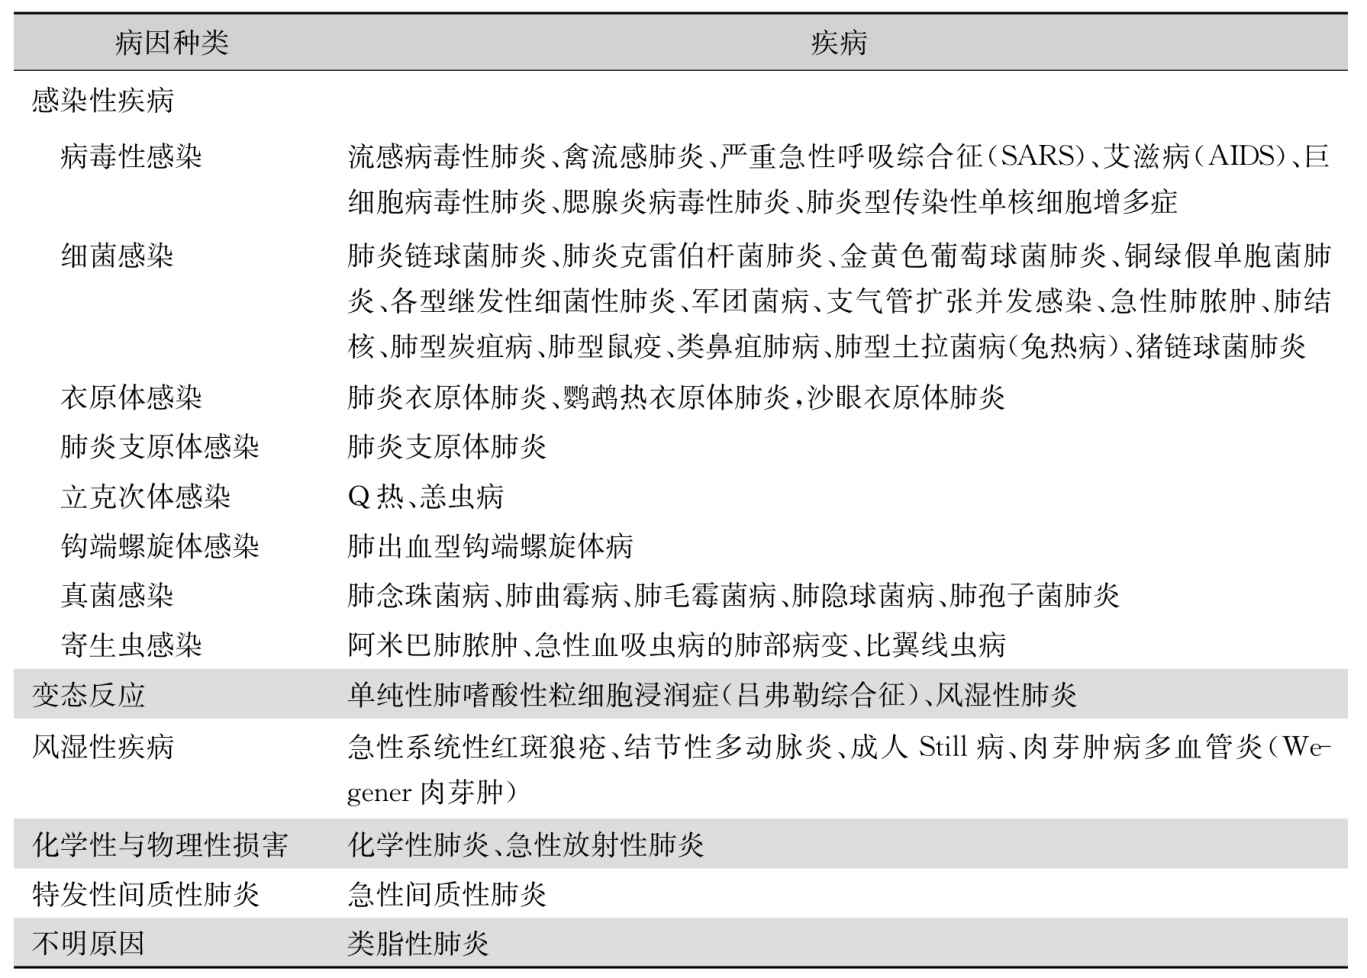
\includegraphics[width=5.95833in,height=4.26042in]{./images/Image00012.jpg}
\end{table}

近年来,机会致病菌性肺炎有增多的趋势。机会感染的致病条件为全身防御能力的严重降低,其诱因为:①基础疾病如恶性肿瘤,肝、肾衰竭,呼吸衰竭,糖尿病,大面积烧伤,白血病,器官移植后免疫抑制剂的应用,遗传性或获得性免疫缺陷综合征(AIDS)等;②附加因素如长期静脉(或膀胱)留置导管,气管插管,长期使用广谱抗菌药物致正常菌群失调,药物或放疗所致白细胞减少或反应性改变,以及T和(或)B淋巴细胞介导的免疫功能降低等。机会致病菌性肺炎有易感性、难治性和反复性等特点,临床症状多不典型,特别在糖皮质激素治疗中可无明显的发热和感染中毒症状。虽用抗生素积极治疗,但常迁延不愈,并发症多。目前革兰氏阴性杆菌已成为医院内机会致病菌性肺炎的重要病原,此外还有嗜肺军团杆菌、非典型分枝杆菌、肺孢子菌、巨细胞病毒、念珠菌、曲霉、隐球菌等致病微生物,经常威胁着患者的生命健康。

\subsection{3.1 感染性疾病}

\subsubsection{3.1.1 病毒性感染}

\paragraph{一、流感病毒性肺炎}

流感病毒性肺炎一般发生于流感流行高峰期间。患者除有流感本身的症状外,发病早期即有呼吸困难甚或发绀。肺部体征为叩诊轻浊音以及由两侧肺底向上蔓延的湿性啰音等。X线检查主要表现为间质性肺炎,并夹杂以不同形态的支气管肺炎样改变,可见肺内斑片状、多叶段渗出性病灶;进展迅速者,可发展为双肺弥漫的渗出性病变或实变,个别病例可见胸腔积液。季节性甲型流感(H1N1、H2N2和H3N2等)所致的病毒性肺炎主要发生于婴幼儿、老年人、慢性心肺疾病及免疫功能低下者,2009年甲型H1N1流感还可在青壮年、肥胖人群、有慢性基础疾病者和妊娠妇女等人群中引起严重的病毒性肺炎,部分发生难治性低氧血症。

流感病毒性肺炎的诊断根据是:①病例发生于流感流行期间,起病较急,在发病早期伴有显著的呼吸系统症状,如咽痛、流涕、咳嗽、呼吸困难,肺部可有啰音等;②血象白细胞数正常或减少;③X线检查肺部有肺炎征象,主要呈支气管肺炎和间质性肺炎表现,也可有肺实变表现;④曾用抗菌药物治疗而未见良效者;⑤鼻咽分泌物或口腔含漱液可分离出流感病毒或病毒抗原、核酸检测阳性。恢复期血清中抗流感病毒抗体滴度比急性期有4倍或以上升高有助于回顾性诊断。

流感病毒性肺炎主要须与肺炎支原体肺炎、肺结核等相区别。

\paragraph{二、高致病性人禽流感病毒性肺炎}

禽流感(禽流行性感冒)是禽类的甲型流感病毒亚型感染。1997年香港特别行政区出现人群暴发禽流感H5N1病毒感染,18例患者中6例死亡,是全球首次发现禽流感病毒能够直接感染人类。目前发现且证实可感染禽类又可感染人类的主要为禽甲型流感病毒H5N1、H9N2、H7N7和H7N9亚型,其中以H5N1亚型引起的病情重,病死率高。2013年3月底华东地区发现的H7N9禽流感病毒是全球首次发现的新亚型流感病毒,至2013年9月底我国内地共报告134例人感染H7N9禽流感确诊病例,其中死亡45人。人禽流感的传染源主要为患禽流感或携带禽流感病毒的鸡、鸭、鹅等家禽,特别是鸡;传播途径主要通过呼吸道,目前尚无人与人之间传播的确切证据。高危人群为与不明原因病死家禽或感染、疑似感染禽流感家禽密切接触人员。人禽流感的潜伏期一般为1~3天,通常在7天以内。临床上多为急性起病,早期表现流感样症状,主要为发热,体温大多持续在39℃以上,热程1~7天,一般为3~4天,可伴有流涕、鼻塞、咳嗽、咽痛、头痛和全身不适。部分患者可有恶心、腹痛、腹泻、稀水样便等消化道症状。重症患者病情发展迅速,可出现肺炎、急性呼吸窘迫综合征、肺出血、胸腔积液、全血细胞减少、肾衰竭、败血症、休克及雷氏(Reye)综合征等多种并发症。体检时重症患者有肺部实变体征。实验室检查外周血白细胞总数一般不高或降低,重症患者多有白细胞总数及淋巴细胞下降。重症患者胸部X线检查可显示单侧或双侧肺炎,少数可伴有胸腔积液等。其影像学特征有:①胸部X线主要表现为肺实质渗出性病变,两肺可见大片状及团絮状高密度影,中心区密度较高,边缘区密度较淡。阴影密度高于常见的病毒性肺炎;②影像学改变变化快,呈游走性;③典型病变病灶累及两肺,大致呈对称性,分布广泛;④临床症状与胸部X线表现不完全相符。病灶吸收落后于临床。诊断依靠流行病学史,结合临床表现和实验室检查,并排除流感、普通感冒、细菌性肺炎、严重急性呼吸综合征(SARS)、传染性单核细胞增多症、巨细胞病毒感染、衣原体肺炎、支原体肺炎等疾病后,可作出临床诊断。确诊有赖于病原学及血清学检测结果,最可靠的方法是从呼吸道标本中分离出禽流感病毒亚型。

\paragraph{三、严重急性呼吸综合征}

严重急性呼吸综合征(SARS)是新出现的传染病是由SARS冠状病毒所致的一种具有明显传染性、可累及多个脏器系统的特殊肺炎。主要通过飞沫、气溶胶或接触污染的物品传播。

潜伏期为2~10日,起病急骤,多以发热为首发症状,体温常>38℃,可有寒战、咳嗽、少痰,偶有血丝痰,心悸、气促,甚或呼吸窘迫。可伴有肌肉酸痛、头痛、关节痛、乏力和腹泻。患者多无上呼吸道卡他症状。肺部体征不明显,部分患者可闻及少许湿啰音,或有肺实变体征。抗菌药物治疗无效。患者的呼吸道症状和肺部体征与胸部X线检查的改变相比常常较轻。实验室检查外周血白细胞计数一般不升高或降低,淋巴细胞减少。胸部X线早期可无异常表现或淡薄阴影,随疾病发展可见不同程度片状、斑片状浸润阴影,或呈网状样改变;部分患者肺部病变进展迅速,呈大片浓密模糊炎性浸润阴影,边缘不清,分布在一个或数个肺叶(段),多为双侧改变,严重者呈“白肺”。肺部阴影吸收消散较慢,与临床体征可不一致。

诊断上强调流行病学史,疑似者可做血清SARS冠状病毒的特异抗体检测和鼻冲洗液或含漱液PCR检测,注意排除上感、流感、细菌性或真菌性肺炎、艾滋病合并肺部感染、军团菌病、肺结核、流行性出血热、肺部肿瘤、非感染性间质性疾病、肺水肿、肺不张、肺栓塞、肺嗜酸性粒细胞浸润症、肺血管炎等临床表现类似的呼吸系统疾病。

\paragraph{四、艾滋病}

艾滋病(AIDS)合并肺部病变引起发热并非少见。有作者提出有下列情况2项或以上者须考虑AIDS肺部病变:①双侧肺门周围网状或网结状阴影;②上述改变在3~5日迅速发展为两肺弥漫性肺间质肺实质浸润甚至为均质性肺实变;③结节样、线条样病变,伴有或不伴有肺门或纵隔淋巴结肿大;④肺部炎症经积极治疗无效甚至病灶发展增多。

如患者同时有下列1项危险因素伴1项相关症状时,即检测抗HIV抗体帮助诊断。

危险因素:①有静脉药瘾史;②有同性恋或异性乱交史;③10年内有输血或输血制品史;④来自流行地区曾与AIDS可疑患者接触史。

相关症状:①长期发热(>1个月)伴体重减轻;②慢性腹泻>1个月;③咳嗽1个月以上,伴气短;④剧烈头痛,甚至出现脑膜刺激征。

AIDS肺部感染的病原体主要有肺孢子菌,此外,巨细胞病毒、弓形虫、隐球菌、类圆线虫、军团菌、肺结核、非结核分枝杆菌等也可引起肺炎,请参阅有关章节。

\paragraph{五、巨细胞病毒肺炎}

巨细胞病毒(CMV)肺炎多发生在免疫抑制宿主,如恶性肿瘤、接受大量免疫抑制剂、细胞毒药物、放射治疗、AIDS等免疫功能低下者易罹患本病。近年器官移植病例增多,特别是肾移植、骨髓移植术后常发生严重的CMV感染,病死率高。如有以下情况,应高度怀疑巨细胞病毒肺炎:①免疫抑制宿主,器官移植受者多发生在术后2~4个月;②发热,体温多在38℃以上;③阵发性干咳,常伴有明显的呼吸困难;④多有全身症状,关节肌肉疼痛、腹胀、直立性低血压等;⑤肺部体征无明显异常;⑥X线胸片早期可能无异常发现,随病情发展逐渐出现双侧弥漫性间质性肺炎或肺泡浸润,肺外周和肺底部常被累及。

确诊需借助实验室检查,常用的检查包括病毒分离、PCR、核酸杂交、抗原血症、DNA血症、mRNA血症等。

\paragraph{六、腮腺炎病毒性肺炎}

国内报告一组成年人流行性腮腺炎并发肺炎的主要表现是临床症状与体征均不显著,仅少数有微热、咳痰或全身不适等症状。胸部X线检查发现肺野内散布有点状、小斑片状或大片状不均匀密度的阴影,通常以右下肺野较为显著,持续时间较长,为48~165天(平均95.7天)。血象无特殊改变。冷凝集试验阴性。磺胺类药物、青霉素、氯霉素治疗均不能使肺部X线征改善。肺部病变大概由于腮腺炎病毒侵犯肺间质及肺泡壁所致。

\paragraph{七、肺炎型传染性单核细胞增多症}

临床症状以发冷、发热、疲乏、淋巴结肿大、咽充血、肌酸痛、头痛、纳差等最为常见。肺炎的表现主要为咳嗽、胸痛,部分病例有血丝痰或铁锈色痰。体检仅1/3病例有肺实变征,但X线检查所有病例均有显著改变。X线胸片所见可分为斑片状、磨玻璃状、堆云状肺部阴影或肺纹理增多,其中以磨玻璃状阴影最具特征性。斑片状阴影与肺炎支原体肺炎所见者相似。病例都有传染性单核细胞增多症的血象,均呈阳性嗜异性凝集反应,经豚鼠肾吸收后,效价在1∶64~1∶2048之间。

此病主要须与肺炎支原体肺炎相区别,二者的X线征可有相似之处,且均可有阳性的嗜异性凝集反应与冷凝集反应,偶尔在传染性单核细胞增多症时,冷凝集试验效价可相当高,故阳性嗜异性凝集反应须经豚鼠肾吸附试验证实或(及)作冷凝集素类型测定,方有鉴别诊断意义。

此外,传染性单核细胞增多症时,血象多有大量的异形淋巴细胞出现,而在肺炎支原体肺炎则无此现象;前者对四环素类抗生素治疗的疗效不确定,也与肺炎支原体肺炎有所不同。表\ref{tab2-9}可作为二者鉴别的参考。
%\begin{table}[htbp]
%\centering
%\caption{肺炎型传染性单核细胞增多症与肺炎支原体肺炎的鉴别}
%\label{tab2-9}
%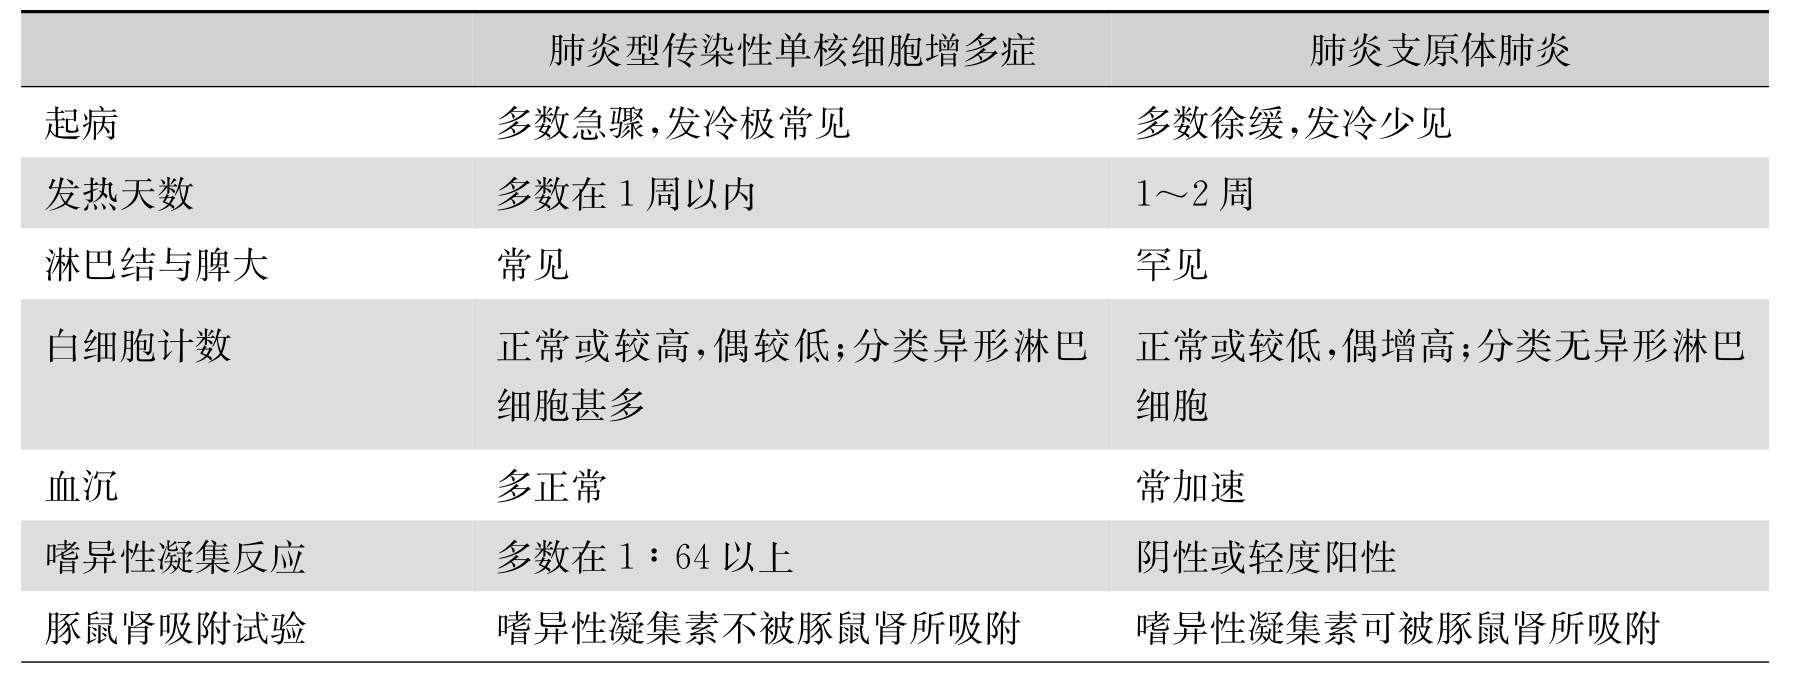
\includegraphics[width=5.96875in,height=2.25in]{./images/Image00013.jpg}
%\end{table}
%续表
%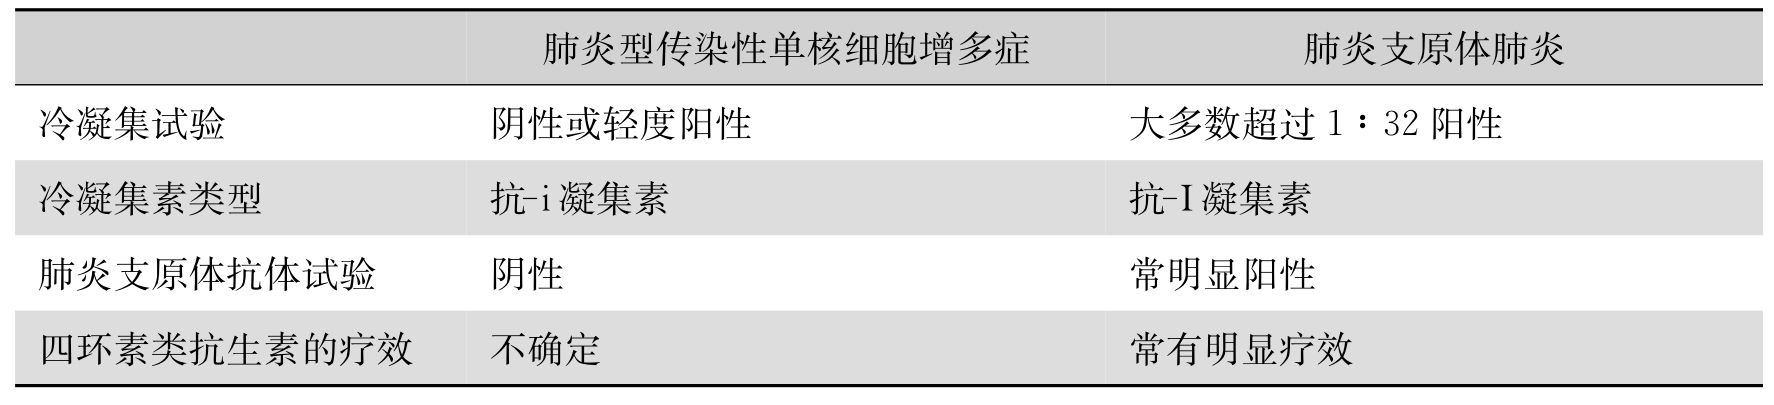
\includegraphics[width=5.90625in,height=1.33333in]{./images/Image00014.jpg}

\begin{longtable}{c}
  \caption{肺炎型传染性单核细胞增多症与肺炎支原体肺炎的鉴别}
  \label{tab2-9}
  \endfirsthead
  \caption[]{肺炎型传染性单核细胞增多症与肺炎支原体肺炎的鉴别}
  \endhead
  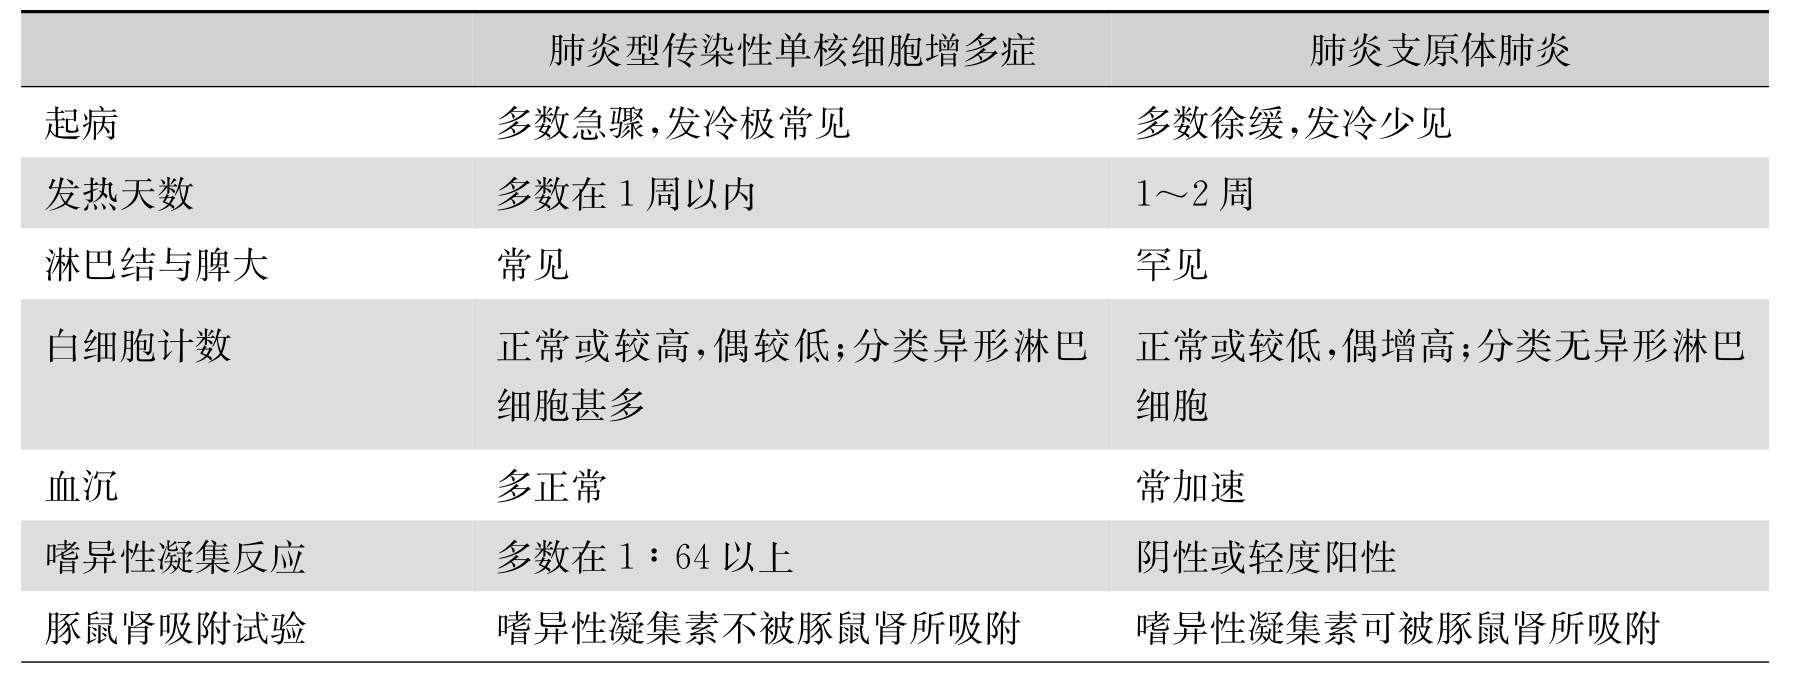
\includegraphics[width=\textwidth,height=\textheight,keepaspectratio]{./images/Image00013.jpg} \\
  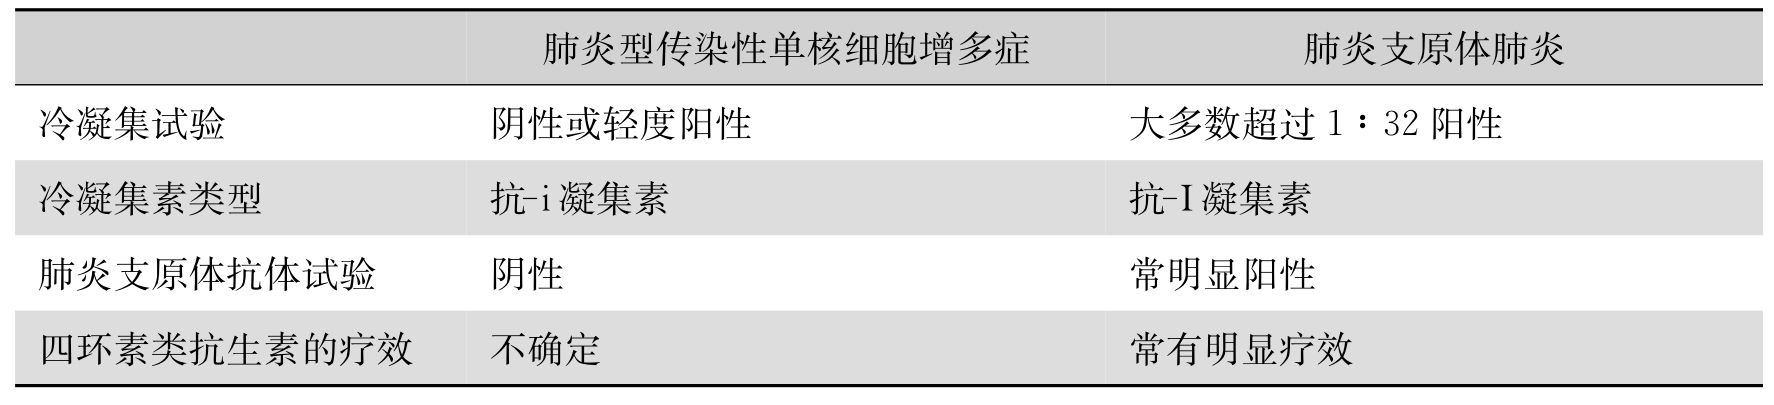
\includegraphics[width=\textwidth,height=\textheight,keepaspectratio]{./images/Image00014.jpg} \\
\end{longtable}

\subsubsection{3.1.2 细菌性感染}

细菌性肺炎的病原体因患病环境不同而有差异。社区获得性肺炎以肺炎链球菌、流感嗜血杆菌、卡他莫拉菌以及非典型病原体常见。医院获得性肺炎除了以上细菌外,还有金黄色葡萄球菌、铜绿假单胞菌、肠杆菌属和肺炎克雷伯杆菌等。病原体可通过空气吸入、血流播散、邻近感染部位蔓延、上呼吸道定植菌误吸、胃肠道反流物误吸和通过人工气道吸入环境中的致病菌引起。细菌性肺炎常以恶寒或寒战、高热起病,呼吸道症状较重,血白细胞增多常在15.0×
10\textsuperscript{9}
/L以上(肺结核可例外),分类以中性粒细胞占优势,并有明显的核左移与中毒性颗粒。血C-反应蛋白和降钙素原升高。

\paragraph{一、肺炎链球菌肺炎}

发病多见于冬春季节,青壮年男性罹患较多。发病前常有受凉、淋雨、饥饿、疲劳、醉酒病毒感染史。起病急骤,多以寒战突然起病,继而高热,多呈稽留热型。颜面潮红,呼吸浅速,甚至出现呼吸困难与发绀。患侧胸痛常见。咳嗽频繁,初为干咳,2~3天后咳出少量黏稠痰液,常呈铁锈色,以后逐渐变为脓性。可有唇疱疹出现。肺部病变部位常可发现轻浊音与捻发音。血象早期呈现白细胞增多、显著核左移与中毒性颗粒。

在病期第3~4天病变侵及整个肺叶,出现明显肺实变体征,浊音界与受累肺叶的境界相一致,听诊发现支气管呼吸音、细湿啰音与捻发音,此时临床诊断更为明确。

肺炎链球菌肺炎早期无特征性表现,凡患者突然畏寒或寒战、高热、胸痛伴肺部呼吸音减弱,白细胞增多,须考虑此病的可能性。胸部X线检查对早期诊断最有帮助。在发病后24~36小时作X线检查,受累肺叶可见有阴影出现,而此时体检可尚无典型的实变体征。此阴影通常从肺门向外周扩展,最后侵及整个肺叶,但目前典型的大叶性病变不多见。痰液涂片染色镜检及培养可证明肺炎链球菌的存在。尿肺炎链球菌抗原可阳性。

近年国内报道的重症肺炎,患者以中、老年人较多,但青壮年者也不少。患者的主要临床表现为高热或体温不升,呼吸困难,明显发绀,白细胞增多或减少,但核左移显著。重症肺炎有时局部体征不明显,甚至有时须经尸检才能证实诊断。

有的病例早期出现意识不清、谵妄、抽搐、昏迷、脑膜刺激征等症状,而肺炎体征尚未显露,易误诊为败血症、流脑、脑炎等疾病。个别病例表现为发热、腹痛、黄疸,可误诊为急性胆囊炎。个别右下叶肺炎患者呈右下腹痛,可误诊为急性阑尾炎。因此凡在肺炎多发的冬春季节,遇见原因未明的急性发热兼有上述表现者,切勿忽略肺炎的可能性,如病情许可应及时做X线检查以明确诊断。

\paragraph{二、肺炎克雷伯杆菌肺炎}

临床特点类似肺炎链球菌肺炎。国内报道的一组病例中,患者都为中年与老年男性,多发于慢性消耗性疾病与免疫力低下的基础上,如原有肺部疾病、糖尿病、手术后和酒精中毒的患者。此病发病急骤,以寒战、高热起病,并有胸痛、呼吸困难与发绀,患者呈急性重病容。神经精神症状也常见。重症病例可迅速发生休克而危及生命。痰为砖红色、血样,或胶冻样类似杨梅果酱,甚黏稠,但也可呈铁锈色。痰中可发现大量肺炎克雷伯杆菌。血象常呈中等度白细胞增多,核左移。肺实变体征可能早期出现,但无典型体征者较常见,甚至X线照片上显示大片致密阴影时,体检仅发现轻浊音和不明显的支气管呼吸音。主要并发症有脓胸、气胸、败血症和慢性肺炎等。

X线检查病变包括大叶实变、小叶浸润和蜂窝状脓肿(坏死性肺炎)形成。大叶实变多位于右上叶,重而黏稠的炎性渗出物使叶间裂呈弧形下坠。免疫功能抑制和慢性肺部疾患者表现为小叶浸润。16\%~50\%伴脓肿形成,形成单个或多个薄壁脓肿,最后遗留广泛性纤维性变或变为迁延性慢性肺脓肿。

临床上遇见年纪较大、全身情况较差的急性肺炎患者,痰中发现较多的疑似肺炎克雷伯杆菌时,应提高警惕。特别是在青霉素治疗下未见好转,肺部病变反而进展时,或在病程中迅速发生休克时,应立即作痰涂片及培养检查。

\paragraph{三、金黄色葡萄球菌性肺炎}

金黄色葡萄球菌引起的急性化脓性炎症。常发生于有基础疾病如糖尿病、血液病、艾滋病、肝病或原有支气管肺疾病者。儿童患流感或麻疹时亦易罹患。年老、体弱、较长期应用广谱抗生素或糖皮质激素等均为发病诱因。

多急骤起病,高热、寒战,发热多呈不规则型或弛张型,胸痛,痰脓性,可早期出现循环衰竭。此病与肺炎链球菌肺炎在临床上的不同点是:败血性经过,热程较长(2~4周),治疗显效后徐缓解热。特征性痰呈脓血性或黏液脓性,与肺炎链球菌肺炎的铁锈色痰有所不同。约半数病例出现皮疹,可为荨麻疹、出血性斑丘疹、瘀斑或瘀点等,而无唇疱疹出现。胸部体征早期不显著,仅呈轻浊音、呼吸音减弱及细湿啰音。胸部体征往往与严重的呼吸困难、发绀、血性痰、休克等症状不相称。

血白细胞增高,中性粒细胞比例增加,核左移并有中毒颗粒。此病的X线特点是:多发性小叶性炎症浸润阴影,但也可为大叶性,病灶内空洞形成、蜂窝状改变或肺气囊肿的出现等,其中尤以后者对诊断更有价值。痰、胸腔积液或血培养的阳性结果,有助于本病的确诊。

临床上如患者有下列表现之一时,须考虑金黄色葡萄球菌性肺炎的可能性:①恶寒或寒战、发热,咳嗽,胸痛,气促,咳脓血痰及伴有皮疹者;②败血症或流感后出现与胸部体征不相称的呼吸困难、发绀等症状,发热迁延不退或退热后又复燃者;③短期内两肺多发性炎症病灶,或一侧肺炎早期即出现肺脓肿、胸膜炎或肺气囊肿者;④已诊断为肺炎,但对青霉素治疗无良好反应者。遇此情况应做细菌学检查,同时加强抗菌药物的应用。

\paragraph{四、铜绿假单胞菌肺炎}

铜绿假单胞菌是医院获得性肺炎的常见病原体,它容易定植于呼吸道,广谱抗菌药物的使用会增加其定植风险。有文献报道4\%~15\%COPD患者痰中可分离到该菌。其近年来发病率呈上升趋势,且由于铜绿假单胞菌极易耐药,并不易为呼吸防御机制杀灭,治疗困难,病死率高。细菌的入侵途径通常是上呼吸道、皮肤与消化道。由于大面积皮肤烧伤合并铜绿假单胞菌感染而引起肺炎者也有时可见。高龄、体弱、原有慢性心、肺疾病、应用广谱抗生素以及器械污染等,是常见的发病诱因。

此病临床上除急性肺炎表现外,往往早期出现谵妄、发绀,并有倒错性发热(即热峰在每天上午出现)及相对缓脉。咳嗽时伴黄脓性痰,少数患者咳出的痰呈浅绿色。重症者可有低血压或休克。胸痛和咯血不常见。肺部X线征是双下肺广泛支气管炎性肺炎,伴有结节状阴影及多发性小脓肿形成,肺脓肿发生较早。

此病经过较重,预后凶险。血流感染发生率低,多见于免疫抑制宿主,因此确诊有赖于痰或胸腔积液的细菌培养。

\paragraph{五、支气管扩张并发感染}

支气管扩张并发急性细菌感染时,患者有发热、咳嗽、咳脓痰等症状,或咯血后出现感染的症状。X线胸片所见类似支气管肺炎、干酪样肺炎或浸润型肺结核。诊断须根据既往病史与治疗效果。如过去屡次在同一部位发生肺炎,则强烈支持支气管扩张合并感染的诊断。此病经积极的抗菌治疗后,往往迅速得到控制,大片阴影逐渐消失,成为索条状卷发阴影。有些感染经治不愈,要考虑是否合并非典型分枝杆菌感染、结核感染等。

\paragraph{六、急性肺脓肿}

急性肺脓肿根据感染途径可分成三个类型:

\subparagraph{(一)吸入性肺脓肿}

大多数肺脓肿主要由于吸入上呼吸道或口腔内带有细菌的分泌物所引起。全身衰弱、受凉、醉酒、中毒、鼻窦炎等常为发病基础。麻醉与手术、食物反流或呕吐、昏迷状态、溺水等均可为诱因,而睡眠中吸入感染则被认为是最常见的诱因。致病菌多为厌氧菌,其他常见菌有化脓性链球菌、金黄色葡萄球菌、肺炎克雷伯杆菌和铜绿假单胞菌等,但往往是多种细菌的混合感染。

患者往往以恶寒或寒战、高热、虚弱、胸痛、心率加快等症状急骤起病。体温常呈弛张热、稽留热或不规则型热。患者大多无呼吸困难与发绀。胸部体征常不显著,但也可呈轻浊音、呼吸音减弱或粗糙、散在性湿啰音等。白细胞显著增多与核左移。只根据胸部体格检查,易忽略肺脓肿的诊断,尤其是深在的肺脓肿往往无明显的体征。炎症浸润破溃后形成脓肿,脓肿向支气管穿破时患者突然咳出大量脓臭痰及坏死组织,静置后多可分为三层:上层为泡沫样痰,中层为黏液样成分,下层为坏死组织。

脓肿分布多位于右肺,右上肺的后段最常累及,其次为左、右下肺叶的背段。X线检查早期可见肺野有单个或多个界限模糊的片状阴影。嗣后此阴影的中心变为圆形透亮区,出现气液平面,转换体位时此气液平面随之改变,据此可以确定肺脓肿的诊断。

\subparagraph{(二)继发性肺脓肿}

某些细菌性肺炎(金黄色葡萄球菌、铜绿假单胞菌和肺炎克雷伯杆菌等)、支气管扩张、支气管囊肿、支气管肺癌、肺结核空洞等继发感染可导致继发性肺脓肿。支气管异物阻塞,也是导致肺脓肿特别是小儿肺脓肿的重要因素。肺部邻近器官的化脓性病变,如膈下脓肿、肾周脓肿、脊柱旁脓肿或食管穿孔等波及到肺也可引起肺脓肿。阿米巴肝脓肿好发于右肝顶部,易穿破膈肌至右肺下叶,形成阿米巴肺脓肿。

\subparagraph{(三)血源性肺脓肿}

通常并发于败血症,特别是金黄色葡萄球菌败血症的病程中。细菌性栓子血行播散到肺,引起小血管栓塞、炎症和坏死而形成肺脓肿。脓肿常为多发性,且常为双侧性。患者在全身感染的基础上发病,常伴高热、寒战、胸痛、咳嗽及血痰。痰量不多,肺部体征不明显。诊断主要依靠X线检查。胸部平片显示双肺多发性圆形病灶。脓肿形成后可见气液平面,有的形成张力性脓腔,可破裂而发生脓气胸。血培养常有致病菌生长,提示脓肿发生在败血症的基础上。也应细致检查其他器官的迁徙性化脓病灶。

\paragraph{七、肺结核}

血行播散型肺结核、浸润性肺结核、空洞性肺结核、干酪样肺炎、结核性胸膜炎等都可引起急性发热与肺部病征,临床上须与其他原因的肺部病变相区别。

\subparagraph{(一)血行播散型肺结核}

亦称急性粟粒型肺结核,多见于婴幼儿和青少年,特别是营养不良、患传染病和长期应用免疫抑制剂导致抵抗力明显下降的小儿,也可见于成人。起病急,持续高热,中毒症状严重。虽然病变侵及两肺,极少有呼吸困难,但也有发生急性呼吸窘迫综合征者。可有全身浅表淋巴结肿大,肝脾大,有时可发现皮肤淡红色粟粒疹和脑膜刺激征。体检时肺部叩诊与听诊体征轻微或缺如,与病情的严重性不相称,如不注意常易致误诊。X线胸片和胸部CT可见由肺尖至肺底呈大小、密度和分布三均匀的粟粒状结节阴影,结节直径2mm左右。参见第28节。

\subparagraph{(二)浸润性肺结核}

属于继发型肺结核,由新发的吸入感染,或由局限性病灶、播散性病灶恶化而成,为活动性肺结核。罹患者多在20~30岁。轻者无明显症状,有些患者呈急性发热,与流行性感冒的临床表现相似,其他为长期微热、心悸、盗汗、乏力、容易烦躁、微咳、咳痰、厌食、体重减轻等中毒症状。

肺部体征因病灶大小、数量及部位而定。病灶小者无异常体征。病灶较大或较多时,可出现轻浊音与细湿啰音(多在锁骨下窝部位)。血沉中等度增速。痰中常可检出结核杆菌。

X线检查显示下列特点:病变部位不定,在成年人多发生在肺尖、锁骨下部;病变多样性,阴影密度较浅,如絮状,边缘模糊,界限不清,可融合和形成空洞。

鉴别诊断上须与肺炎支原体肺炎、不完全性大叶性肺炎、肺吸虫病、支气管扩张合并感染等相区别。

下肺结核 下肺结核临床上少见,可见于艾滋病、糖尿病和其他免疫抑制患者的肺结核,病变位于肺门以下,发病右下叶多于左下叶。咯血是常有的症状;全身中毒症状与一般上肺结核无差异,但病程发展较快。发病常类似支气管肺炎。X线阴影特征与一般肺结核相同,但以大片状广泛浸润为多,且在早期即可有肺不张与空洞形成。早期诊断往往较为困难,最易误诊为肺脓肿与肺炎,有时甚至被误诊为肺包虫病。下列几点有助于早期鉴别诊断:

1.下肺结核患者有恶寒、寒战者少见。咳嗽与胸痛一般较肺炎或肺脓肿为轻,脓痰不多见,病程则较肺炎或肺脓肿为长。

2.大多数下肺结核患者的白细胞总数在正常范围内。

3.肺脓肿与下肺结核好发部位虽然都在肺下叶背段,但青年患者在下叶背段有空洞性病变,而症状与肺脓肿不尽相符时,应注意下肺结核的可能性。

4.下肺结核诊断的主要根据是痰中查得结核杆菌,应反复进行痰集菌涂片检查,必要时作培养或动物接种。

5.相当数量的下肺结核患者同时有支气管内膜结核,支气管镜检查是诊断的重要方法之一。

\subparagraph{(三)空洞性肺结核}

亦属于继发性型肺结核,临床症状较多,发热,咳嗽,咳痰和咯血等。空洞形态不一,可呈虫蚀样空洞、薄壁空洞、厚壁空洞、张力性空洞以及干酪溶解性空洞等,多有支气管播散病变。空洞内一般无气液平面,空洞周围炎性病变较少,常伴有条索、斑点及结节状病灶。痰中一般容易检到结核杆菌。合并肺炎时,应与肺脓肿相鉴别。

\subparagraph{(四)干酪样肺炎}

亦属于继发型肺结核,与浸润性肺结核不同,主要是干酪样变化比病灶周围炎变化显著,进展急剧,是严重的结核病类型。干酪样肺炎起于结核杆菌的支气管播散,在机体抵抗力极度降低和对结核杆菌过敏反应增高的情况下发病,临床与病理上可区分为大叶性干酪样肺炎与小叶性干酪样肺炎两种:

\hypertarget{text00025.htmlux5cux23CHP2-7-1-2-7-4-1}{}
1.大叶性干酪样肺炎

发病急,与肺炎链球菌肺炎相似,但温度上升较慢,经2~3天升至39~40℃,逐渐转为弛张热,并有恶寒、呼吸困难、胸痛、咳嗽、咳痰、痰中时有带血、纳差、极度疲乏等症状。体检可发现呈大叶分布的肺实变体征。X线检查发现大片阴影,数周后可溶解形成空洞,呈虫蚀样空洞。血象白细胞计数正常或轻度增多。大部分于发病一个月左右痰中发现结核杆菌。此病主要须与非结核性大叶性肺炎(主要是肺炎链球菌大叶性肺炎)相鉴别。干酪样肺炎发病较后者为慢,无唇疱疹,无铁锈色痰,颜面苍白而非潮红,痰中可找到结核杆菌,血中白细胞数通常在15.0×10\textsuperscript{9}
/L以下,对青霉素疗效不佳,且患者发病前往往已有食欲欠佳、消瘦、潮热、盗汗等结核全身中毒症状。由于此病经过严重,凡遇到大叶性肺炎而疑为结核性时,应即积极进行抗结核治疗,以免耽误病情。干酪样肺炎兼有空洞时须与肺脓肿相鉴别,前者有空洞形成时痰中应找到结核杆菌。

\hypertarget{text00025.htmlux5cux23CHP2-7-1-2-7-4-2}{}
2.小叶性干酪样肺炎

多见于病程长、治疗效果不佳、全身情况及抵抗力很差的慢性肺结核患者,或发生于并发糖尿病的肺结核患者,主要病变是散布于两肺的多数性干酪样病灶。这些病灶可同时或分批出现。X线胸片上显示大小不一、边缘模糊的阴影.可能为3~5片至7~8片不等。上述情况的患者如突然发生急性肺部感染的症状,如畏寒、发热、咳嗽、咳痰、脉快、呼吸困难、发绀等时,应考虑小叶性干酪样肺炎的可能性。体检可发现两肺散在性干性与湿性啰音,但叩诊浊音不显著。小叶性干酪样肺炎早期与非结核性小叶性肺炎不易鉴别,主要鉴别根据为前者血中常无白细胞增多,或仅轻度增多,而后者常有明显的白细胞增多;前者痰中常可找到结核杆菌而后者则无。

\paragraph{八、军团菌肺炎}

本病首次在美国(1976年)发现,近年国内多处亦发现有散发病例,还曾有暴发性流行。潜伏期2~10天。临床表现为倦怠、头痛、肌痛、发热(可达40℃或以上)和相对缓脉等,可有畏寒或寒战,或不同程度的消化道症状与精神神经症状。咳嗽逐渐出现并加剧,伴胸痛与咳黏液痰,痰数日后转为脓性。突出的血生化改变为低钠血症与低磷血症。部分病例可合并肝功能损害。典型X线胸片为早期一侧肺下野出现境界不清的浸润阴影,多呈斑点状间质浸润或致密性实变。其后扩大至一侧肺下野乃至一侧肺野。部分病例可累及双肺。1/3~2/3病例有不同程度的胸腔积液。患者痰液、胸腔积液和气管吸出物中均可检出军团菌。血清特异性免疫学检查亦有助于诊断。尿军团菌抗原及呼吸道分泌物直接荧光抗体染色法有助于本病早期诊断,前者敏感性是80\%~90\%,特异性是98\%~100\%,检测时间小于1小时,但后者敏感性较低。聚合酶链式反应(PCR)也有助于诊断,血、尿标本的敏感性为75\%~82\%,特异性90\%~100\%。诊断上本病与其他社区获得性肺炎相比较,头痛、腹泻、肌酸激酶值升高、严重低钠(<130mmol/L)、肝功能异常、对β-内酰胺类抗生素不敏感在军团菌肺炎中多见。1998年温思罗普大学发表了温思罗普大学医院(WUH)标准,以便于区分军团菌肺炎和其他细菌感染的肺炎(表\ref{tab2-10}\footnote{≥10分=临床诊断;5~9分=疑诊;<5分=排除。例1是临床诊断,例2为疑诊,例3排除})。但回顾性分析发现该标准能较好的区分军团菌肺炎和其他细菌感染的肺炎,但假阳性率较高。如用大环内酯类及氟喹诺酮类等药物治疗有效也支持诊断。另外,治疗后临床症状好转而胸片仍进一步恶化也是本病的特点之一。Fiumefreddo等提出另一社区获得性军团菌肺炎的临床诊断评分,分别是发热、无痰、血钠降低、LDH升高、C-反应蛋白升高和血小板降低6个指标,每项1分共6分,分值越高军团菌病可能性越大,≥4应高度怀疑军团菌病,此评分与WHU标准相比更为简单易用。其他还有CBPIS军团菌病评分系统也可应用(Clinical
Infectious Diseases.2003;37:483-9)。

\begin{table}[htbp]
\centering
\caption{WUH军团菌病评分系统}
\label{tab2-10}
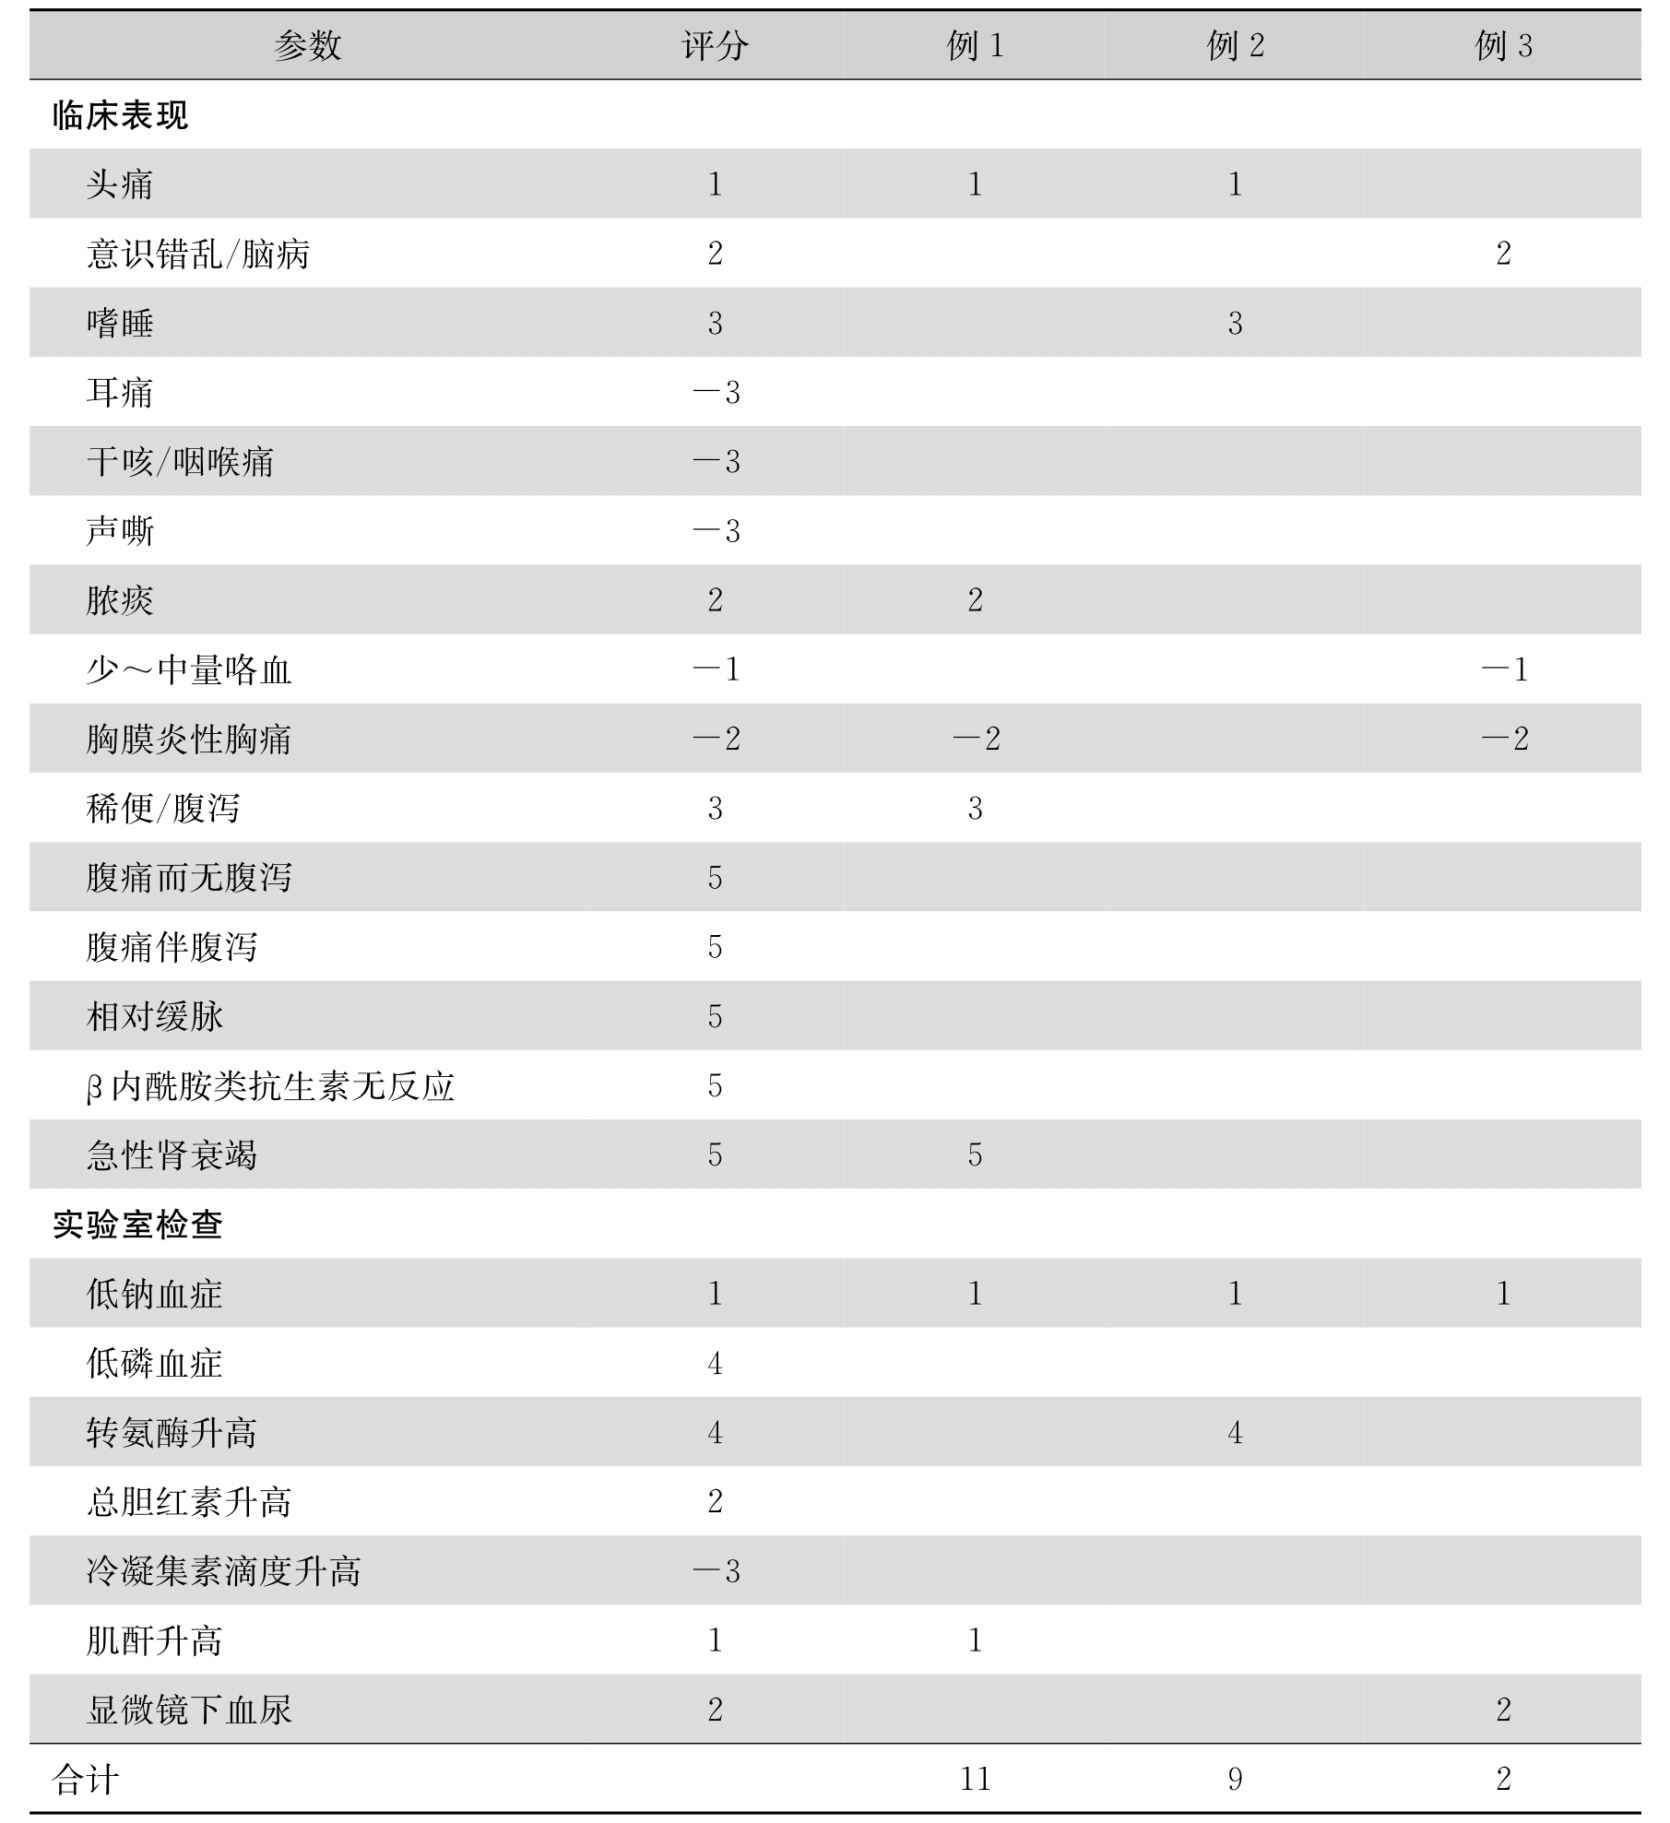
\includegraphics[width=6.03125in,height=6.58333in]{./images/Image00015.jpg}
\end{table}


据近年一组37例患者的综合分析,35\%有胃肠、肝、肾和神经精神异常的肺外症状,38\%有低钠血症,40\%合并胸腔积液,17\%合并肺脓肿。由此可见本病临床表现为全身性症状和呼吸系统症状。X线胸片肺部病变的恢复迟于临床改善,有些病例仍有进展。

\paragraph{九、肺型炭疽病}

诊断炭疽病须注意流行病学史。此病是重要职业病之一,主要见于从事畜牧、皮毛、毛织等职业的人,或曾与病畜接触的人。近年有用于生物恐怖活动。肺型炭疽病的发生是由于吸入混有炭疽杆菌芽胞的尘埃而致感染,又称“吸入性炭疽”,预后很差,但临床上少见。凡遇有急性发热患者伴有肺部感染症状,咳泡沫样血痰而兼有上述流行病学史者,须考虑有肺型炭疽病的可能性。

发病急骤,有寒战、高热、咳嗽、胸痛、大汗、心率增速、气促、喘鸣、发绀等症状,继而咳出锈色或血样痰。患者神志一般清醒。重症者发绀显著,血压下降,脉搏细速,有明显的休克现象。肺部体征仅可闻及散在的细湿啰音,或有胸腔积液征。体征与病情严重程度不成正比。血象白细胞数增高。

确诊须依靠细菌学检查。痰与胸腔渗出液直接涂片,均可发现革兰氏染色阳性、具有荚膜的粗大的炭疽杆菌。培养也容易获得阳性结果。

\hypertarget{text00025.htmlux5cux23CHP2-7-1-2-10}{}
十、肺型鼠疫

鼠疫是危害人类最严重的烈性传染病之一,病原体为鼠疫杆菌,传染源为受感染的鼠类或其他野生啮齿类动物。

鼠疫潜伏期多为2~3天,甚少超过5天。肺型鼠疫可分原发性与继发性两种。前者于发病后即出现肺部征象,表现为急性肺-胸膜炎;后者则继发于腺鼠疫之后。

肺型鼠疫发病急骤,患者有寒战、高热、胸痛、咳嗽、咳痰。痰最初为黏液性,后变稀薄稍带泡沫,不久可成为鲜红色血样,痰中含大量鼠疫杆菌。呼吸困难与发绀迅速出现。肺部体征多不明显,有时可发现肺部局限性浊音、散在性湿啰音与捻发音、胸膜摩擦音。X线检查可为正常或仅发现轻微病变,往往与病情的严重性不相称。肺型鼠疫常发展为败血症,未接受及时有效治疗者常于2~3日内死于心力衰竭、出血、休克,病死率高达70\%~100\%。

凡在鼠疫可能发生的地区和环境,遇有急性肺部感染患者,有明显的中毒症状、早期衰竭,或同时有淋巴结肿痛及出血现象,应考虑此病的可能性。痰液细菌学检查(包括涂片及培养)容易获得阳性结果,对确诊提供可靠依据。

\hypertarget{text00025.htmlux5cux23CHP2-7-1-2-11}{}
十一、类鼻疽肺病

类鼻疽是类鼻疽伯克霍尔德菌(类鼻疽假单胞菌)引起的人兽共患传染病,主要通过污染的水源、土壤经破损皮肤传染,或经污染的食物由消化道传染。其发病具有地域性分布,主要在热带和亚热带,属于地方性传染病,我国海南、广东、广西、福建、香港、台湾是多发地区。类鼻疽病多发于中年(22~66岁,平均47岁)男性,农民与渔民多见,大多有基础疾病,如糖尿病、继发型肺结核和类风湿关节炎等。畏寒、发热见于所有患者。急性肺部感染是类鼻疽病的最常见类型,约占70.5\%,可为轻症的肺炎至严重的坏死性肺炎。起病多急骤,恶寒或寒战、高热(多呈稽留热)、头痛、全身肌痛、胸痛、干咳或有咯血,呼吸困难、休克和败血症等,体检有局部皮肤脓肿、肝脾和淋巴结肿大,肺部体征少,可有湿啰音。大多患者血白细胞升高,中性粒细胞占优势。半数患者有肝功能损害,71\%血培养类鼻疽假单胞菌阳性。胸部X线大多数为肺上叶病变,有浸润病灶及(或)空洞,空洞多为单发,大小差异很大,少有液平,常可与肺炎、肺结核或其他慢性肉芽肿疾病混淆。确诊主要依靠病原菌分离及血清学检查。病原学标本可来自血液、脓肿液、痰液和尿液等,血清学检查则用标准类鼻疽伯克霍尔德菌诊断血清,类鼻疽特异性抗体可阳性。

\hypertarget{text00025.htmlux5cux23CHP2-7-1-2-12}{}
十二、肺型土拉菌病(兔热病)

土拉菌病一般发生在夏季,潜伏期通常为1周。起病急骤,体温迅速上升达39~40℃,伴全身乏力,畏寒,头痛,背痛,全身肌痛。病情发展时出现谵妄、昏睡、烦躁不安等急性全身中毒症状。患者体温升高持续2~5天,随之徐缓下降。细菌侵入部位的局部淋巴结首先有痛感,2天内皮肤呈现原发性病灶,多发于手或手指。开始呈红丘疹,继而发生脓疱,破溃后,形成中心性坏死,逐渐变成边缘较硬的溃疡。肿大的局部淋巴结,亦可破溃。病程一般持续3~4周,恢复缓慢,约需2~3个月或更长。伤寒型(全身型或胸膜肺型)的土拉菌病是一种小叶性肺炎,病程为迁延性(1~2个月或更长),有时痰中带血,有化脓的倾向。患者常有较轻的中毒症状,肺部体征不明显,无唇疱疹及显著的白细胞增多,但往往并发干性或渗出性胸膜炎。诊断依靠流行病学史及细菌血清学检查。

\subsubsection{3.1.3 衣原体感染}

衣原体是一种介于病毒、细菌和立克次体间的微生物,更近似于细菌,其大小约0.2~0.4μm。可引起肺炎的衣原体主要有肺炎衣原体(TWAR)和鹦鹉热衣原体两种,少数由沙眼衣原体引起。

\paragraph{一、肺炎衣原体肺炎}

肺炎衣原体可引起上呼吸道感染,如鼻窦炎、中耳炎和咽炎,也可引起下呼吸道感染,如支气管炎和肺炎。近年肺炎衣原体肺炎患病率有增高的趋势,多感染儿童和老年人,占社区获得性肺炎的6\%~19\%,国内近年报道一组665例社区获得性肺炎肺炎衣原体占6.6\%。起病多隐袭,早期表现为上呼吸道感染的症状,如声嘶、咽痛、发热等,症状通常较轻,数天或数周后患者上呼吸道症状减退,开始出现咳嗽,提示下呼吸道受累。其他症状有肌痛、头痛、不适和乏力。重症感染可有脓痰、呼吸困难等,多见于COPD和心力衰竭患者。可伴有肺外表现如中耳炎、结节性红斑、心内膜炎、关节炎、甲状腺炎、脑炎和吉兰-巴雷综合征等。X线胸片显示肺叶或肺段的浸润病灶,多见于下叶。

病原体分离培养、聚合酶链反应、血清学试验如微量免疫荧光(MIF)抗体试验和补体结合(CF)抗体试验等有助于确诊。本病需与病毒性肺炎、支原体肺炎、流行性感冒、肺结核、真菌感染等鉴别。

\paragraph{二、鹦鹉热衣原体肺炎}

鹦鹉热衣原体寄生于鹦鹉、鸽、鸡等100余种家禽和野生鸟类体内,主要感染禽类和低等哺乳类动物,人类并不常见。通常发生于与受感染鸟密切接触者,感染途径为通过呼吸道吸入疫鸟排泄物气溶胶所致。病原体吸入体内后首先进入肝脾的网状内皮细胞进行增殖,再经血路进入肺和其他器官,所以人类的鹦鹉热既可以是呼吸道感染,也可能是以呼吸道为主的全身感染。

起病多隐袭,病情轻者如流感样症状。重症肺炎者多有寒战、发热、体温逐渐升高,第1周内可达40℃以上,热程3~4周,伴乏力、头痛、关节肌肉疼痛,亦可有结膜炎、口腔炎、鼻出血或出现类似伤寒的玫瑰疹。1周左右才出现呼吸道症状,如咳嗽、少量咳痰或痰中带血,病变严重者可有呼吸困难及发绀。病程中尚可出现纳差、恶心、呕吐、腹痛、腹泻等消化道症状,心肌炎、心内膜炎及心包炎,亦可有嗜睡、谵妄、木僵、抽搐、意识不清等神经精神症状。体检肺部体征常较症状轻,病初可无明显体征,以后可有湿啰音,少数患者可有肺实变征或胸腔积液征。X线胸片显示早期从肺门向外放射的浸润病灶。病灶可融合呈叶性分布,以下叶多见。常有弥漫性支气管肺炎或间质性肺炎的X线表现。肺内病变吸收缓慢。

本病确诊须依靠衣原体分离培养及(或)特异性血清学检查。PCR诊断效果更佳。本病需与病毒性肺炎、支原体肺炎、流行性感冒、肺结核、真菌感染等鉴别。与肺炎衣原体肺炎的鉴别主要是后者通常无鸟类接触史,临床症状较轻,体温很少超过37.8℃,且很少累及呼吸道以外器官。微量免疫荧光(MIF)抗体试验可用于鉴别不同的衣原体。

\paragraph{三、沙眼衣原体肺炎}

沙眼衣原体包括15个血清型,引起人类沙眼、性病淋巴肉芽肿、包涵体性结膜炎、生殖道感染,以及新生儿肺炎。在极少数情况下,沙眼衣原体也引起免疫缺陷成人患者的呼吸道感染,甚至正常成人的社区获得性肺炎,病因不清。

沙眼衣原体新生儿肺炎主要见于2~12周新生儿及婴儿,通过感染的母亲产道时受感染。大多数无发热,起始症状通常是鼻炎、伴鼻腔黏液性分泌物和鼻塞。随后发展为断续的咳嗽,呼吸急促和肺部啰音,可伴有心肌炎和胸腔积液。肺部X线显示间质浸润。半数患儿可伴有急性包涵体性结膜炎。

\subsubsection{3.1.4 支原体感染}

支原体是介于细菌和病毒之间,能独立生存而不需要寄身于其他生物细胞的最小微生物,目前已知的支原体有80余种。

肺炎支原体肺炎

由肺炎支原体感染引起的肺炎称为肺炎支原体肺炎,此病秋冬季节多见,但季节性差异并不明显。青壮年较易罹患。国内调查占社区获得性肺炎的20.7\%,且多合并其他细菌感染。潜伏期1~2周,缓慢起病,发热呈中等度,多持续约1~2周,也可持续3周。咽痛与咳嗽是常见的症状,发病初期以阵发性干呛性咳嗽为主,以后约半数病例可咳少量黏液痰或痰中带血丝,或小量咯血,而无铁锈色痰。这种呛咳和痰的特征是大叶性肺炎所少见。全身症状较为明显,如乏力、头痛、咽痛、纳差、腹泻、肌痛、耳痛等。体格检查肺部体征与X线征不相称,虽X线检查有显著的改变,但肺部实变征象却不明显。

血象白细胞总数多数正常,分类可呈相对性淋巴细胞增多与轻度或中等度嗜酸性粒细胞增多,这与细菌性肺炎的鉴别有一定意义。血清冷凝集反应阳性率高达80\%,效价达1∶32或以上有诊断价值,于病程第2~3周阳性率较高。血清支原体IgM抗体≥1∶64,或恢复期抗体滴度有4倍升高,可进一步确诊。直接检测呼吸道标本中肺炎支原体抗原,可早期快速诊断。

X线检查肺部阴影往往在发病后2~5天出现,通常有下列三项特点:①肺纹理增多;②沿增多的肺纹理出现不规则的斑片状实质阴影;③多数改变集中于肺门附近。病变所在以下叶为多。上述的X线征大多于1~4周内消散。单纯依靠X线检查往往难于与不完全性大叶性肺炎、浸润型肺结核、癌性淋巴管炎等相区别。

肺炎支原体肺炎的诊断须综合全面检查结果而确定。主要根据是:①急性肺部感染具有感冒样症状,阵发性呛咳以及全身性症状;②X线检查有上述的改变;③血清冷凝集反应滴度在1∶32或以上,及(或)血清肺炎支原体IgM抗体滴度≥1∶64,或有4倍以上升高;④青霉素治疗无效而大环内酯类、氟喹诺酮类和四环素类抗生素有良好疗效;⑤有条件时可从痰或咽洗液中分离出肺炎支原体。近年有作者认为PCR技术可为肺炎支原体感染提供早期快速敏感特异的病原学诊断方法。

此病最易误诊,由于肺部实变征不明显,如无X线检查易误诊为流感或急性上呼吸道炎、支气管炎。有时患者因急性发热兼有上呼吸道炎症状,经常规X线胸部检查而发现。

\subsubsection{3.1.5 立克次体感染}

立克次体是介于细菌和病毒之间的微生物,有类似一般细菌的形态和结构,绝大多数又具有与病毒相似的在宿主细胞内才能生长、繁殖的特性。

\paragraph{一、Q热}

Q热是由Q热立克次体(贝纳柯克斯体)引起的急性传染病,大部分患者有间质性肺炎。许多野生动物、家畜、家禽都可自然感染。与病畜或其排泄物接触或饮用其生乳为主要的感染方式。

潜伏期9~26天,平均为10~14天,但在吸入感染时可缩短至3天。患者多以恶寒、高热而急骤发病。发热呈弛张热型,一般持续5~14天左右,然后迅速下降或于2~3天内降至正常。少数热程可持续3个月以上。剧烈的持续性头痛往往是此病的特征,肌痛与关节痛也常见。但与其他立克次体病不同,此病无皮疹,外斐试验阴性。

间质性肺炎通常在病期第3~4天出现。患者虽有肺部感染,但一般只有轻微的咳嗽,无痰或咳少量黏液性痰。胸部X线检查显示均匀模糊阴影,多侵及一个肺叶,尤以左下肺叶为多见。此病的特点是肺部体征多不明显或缺如,一般也无明显的呼吸道症状,但X线检查常能发现肺部有炎症。往往呈相对性缓脉,冷凝集试验阴性。

Q热的确诊须依靠病原体分离与血清免疫学检查。补体结合试验在病程第7~10天开始阳性(1∶32~1∶64),滴度逐渐上升,至第20~30天达高峰(1∶160~1∶640),以后逐渐下降。毛细管凝集试验的敏感性和特异性均较高。间接免疫荧光试验的抗体效价1∶64~1∶128或双份血清抗体效价升高4倍以上有诊断意义。

本病主要须与肺炎支原体肺炎相区别。肺炎支原体肺炎有较明显的上呼吸道症状,冷凝集试验常为阳性,但最可靠的鉴别方法仍为Q热立克次体分离或补体结合试验。

本病与布鲁菌病的传染源及传播途径有共同点,故二者混合感染亦有之。

\paragraph{二、恙虫病立克次体肺炎}

恙虫病的组织病理变化主要在血管系统,可见局灶性或广泛性血管炎、血管周围炎和血栓形成,导致全身多脏器损害,其中肺部损害较为常见,表现为肺充血、出血性肺炎或继发性支气管肺炎。

恙虫病临床特点为突然起病、高热、皮疹、淋巴结肿大、肝脾大和焦痂等。肺炎者主要表现为咳嗽,多为干咳或轻咳,可有咳少量白色黏痰、胸闷、胸痛,严重时可出现间质性肺炎,以呼吸困难为主,可出现发绀、急性呼吸衰竭。肺部体检可有湿啰音,少数有干啰音,或仅肺部呼吸音变粗。X线胸片提示肺浸润,双侧多见。肺间质炎症改变表现为肺纹理增多及模糊,呈网状影,并有小斑点病变。肺部炎性渗出病变表现为增粗肺纹理间可见斑片状、小片状、部分呈大片状密度均匀、边缘模糊阴影。可有肋膈角变钝与胸腔积液。合并急性肺损伤/急性呼吸窘迫综合征(ALI/ARDS)者胸部X线可表现双肺弥漫性浸润阴影、磨砂玻璃样改变。

恙虫病诊断上具备以下其中3项者可作诊断:①有野外接触史;②高热并发现特征性焦痂或溃疡;③淋巴结肿大、皮疹;④外斐试验1∶160以上。肺部合并症者除符合恙虫病诊断标准,有肺部临床表现和胸部X线改变外,需注意排除其他肺部疾患,如支原体肺炎、肺炎链球菌肺炎、浸润性肺结核等。

\subsubsection{3.1.6 螺旋体感染}

肺出血型钩端螺旋体病

肺出血型钩端螺旋体病即钩端螺旋体性出血性肺炎,是近年来比较多见的急性感染。患者多无黄疸,肝、肾损害较不显著,较易误诊。

据一组对43例患者资料总结的报道,大多起病急骤,有恶寒或寒战、高热、头痛、全身肌痛等症状,类似流行性感冒;部分起病较缓,仅轻微发热伴有鼻咽部症状,易与轻症流感或急性上呼吸道感染相混淆。2~3天后出现咳嗽、痰中带血、咯血、胸闷、气促及轻度发绀。有的病例发生大咯血,引起严重呼吸困难、发绀甚至窒息。患者肺炎症状虽显著,但胸部体征较少,仅部分病例叩诊呈轻度浊音和闻及湿啰音。患者通常并发心肌炎,表现为胸闷、脉搏加速与心电图改变。

X线征常在病程4~11天出现,也可较早或较迟,胸片上呈现双侧肺野斑片状模糊阴影,以中、下肺野尤著,其性质大多属于出血性炎症性实质性病变。胸部CT可见多形态变化表现,可早期发现X线胸片没有显示肺内出血改变,亦可显示病灶形态与分布范围,能判断肺部出血的程度。值得注意的是,部分病例在出血性肺炎症状尚未出现前已有异常的X线征,为早期诊断提供重要根据。

在有钩端螺旋体病的地区,值夏、秋季流行季节,遇有类似流感或急性上呼吸道感染患者,须警惕此病的可能性。患者发病前3~20天曾与疫水有接触史,尤其是初到该地区者,对提示诊断有重要意义。若患者已出现出血性肺炎症状,则可能性更大,但须与其他原因的肺炎、肺结核相鉴别。胸部X线检查对鉴别诊断帮助颇大,确诊须依靠病原学与血清学检查。

\subsubsection{3.1.7 真菌感染}

肺部真菌感染是最常见的深部真菌病。罹患者多有接受广谱抗生素、糖皮质激素、细胞毒药物或免疫抑制剂等治疗;或有慢性基础疾病如糖尿病,心、肺、肾、肝等疾病;或人免疫缺陷病毒(HIV)感染或艾滋病者。故诊断时应详细询问病史和用药史。从患者危险因素、临床特征、微生物学和组织病理学进行诊断分级,见表\ref{tab2-11}\footnote{\textsuperscript{a}
包括影像学;+:有,-:无;b肺组织、胸腔积液、血液真菌培养阳性;c除确诊标准外,也包括特异性真菌抗原检测阳性及合格的深部痰标本连续≥2次分离到同种真菌}。

\begin{table}[htbp]
\centering
\caption{侵袭性肺真菌病的分级诊断标准}
\label{tab2-11}
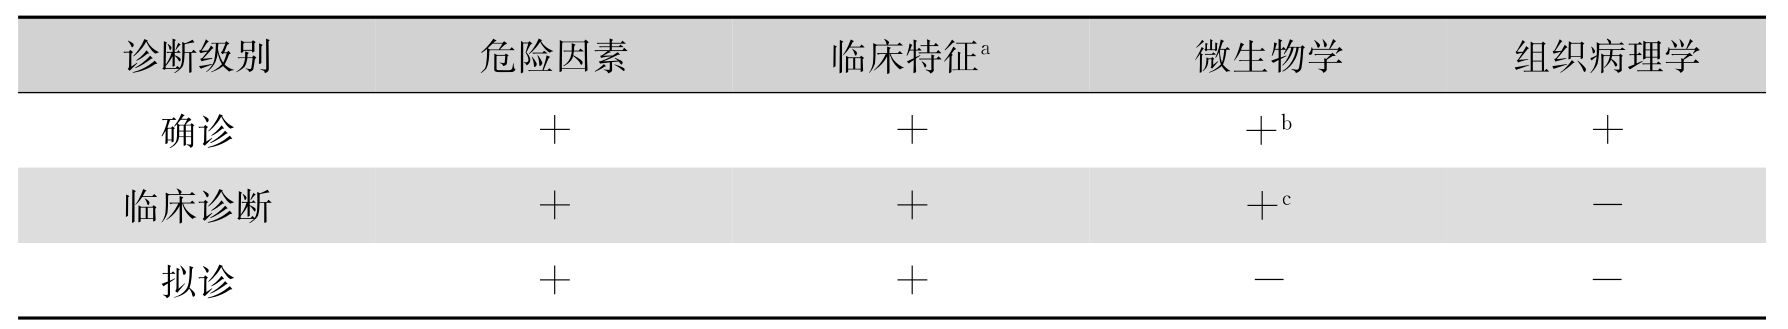
\includegraphics[width=5.94792in,height=1.08333in]{./images/Image00016.jpg}
\end{table}



\paragraph{一、肺念珠菌病}

有关肺念珠菌感染在临床上是多见还是很少见的问题一直存在争议。我国16家医院参加的肺真菌病调查显示该病仅次于肺曲霉病,位列第二。此病为白念珠菌或其他念珠菌所引起的急性、亚急性或慢性肺炎。感染途径主要是吸入,其次为血源性播散。临床上分为念珠菌支气管炎和念珠菌肺炎。支气管炎型表现为阵发性刺激性咳嗽,咳多量白泡沫塑料状稀痰,偶带血丝,随病情进展,痰稠如干糨糊状。憋喘、气短,尤以夜间为甚。乏力、盗汗,多不发热。X线仅示两肺中下野纹理增粗。肺炎型多发于免疫功能低下的患者,表现为畏寒、高热,咳白色泡沫黏痰,有酵臭味,或呈胶冻状,有时咯血,临床酷似急性细菌性肺炎。胸部X线显示双下肺纹理增多,纤维条索影伴散在的大小不等、形状不一的结节状阴影,呈支气管肺炎表现;或融合的均匀大片浸润,自肺门向周边扩展,可形成空洞。双肺或多肺叶病变,病灶时有变化,但肺尖较少受累。偶可并发渗出性胸膜炎。

诊断肺念珠菌病,要求合格的痰液或支气管分泌物标本2次显微镜检酵母假菌丝或菌丝阳性,以及真菌培养连续2次以上有同一菌种生长。另外,血清1,3-β-D-葡聚糖抗原检测连续2次阳性可做诊断参考。组织活检见有念珠菌菌丝侵入及炎症细胞浸润,可以确诊。

\paragraph{二、肺曲霉病}

肺曲霉病主要由烟曲霉引起,临床上主要有五种类型:侵袭性肺曲霉病、气管支气管曲霉病、慢性坏死性肺曲霉病、曲霉肿和变应性支气管肺曲霉病(ABPA)。这些类型的病变临床表现并不一样。

侵袭性肺曲霉病是最常见的类型,症状以干咳、胸痛常见,部分患者有咯血,病变广泛时出现气急和呼吸困难,甚至呼吸衰竭。部分患者可有中枢神经系统感染。中性粒细胞缺乏患者其X线胸片显示以胸膜为基底的多发的楔形阴影或空洞,病变早期胸部CT为晕轮征(halo
sign),后期为新月体征。但慢性阻塞性肺疾病合并侵袭性曲霉病时典型的CT改变很少见,而非特异性肺实变更多见。

气管支气管曲霉病病变主要在大气道,症状为发热、频繁咳嗽、少痰、胸痛、咯血。支气管镜检可确诊,可见气管支气管内假膜、溃疡、结节等病变。

慢性坏死性肺曲霉病亦称半侵袭性肺曲霉病,患者有长期呼吸道症状如咳嗽、咳痰等,也多有发热。X线显示慢性肺部空洞性病变。

曲霉肿(曲菌球)常继发于支气管囊肿、支气管扩张、肺脓肿和肺结核空洞。继发感染时可有发热,症状主要是刺激性咳嗽,常反复咯血,甚至大咯血,痰量一般不多。X线胸片显示在原有的慢性空洞内有一随体位改变而在空腔内移动的团球影。

ABPB为对曲霉过敏者吸入大量孢子后出现发热、喘息、畏寒、乏力、刺激性咳嗽、咳棕黄色脓痰,偶带血。患者多有哮喘病史。哮喘样发作为其突出的临床表现。X线胸片为上叶短暂性实变或不张,一过性肺浸润,磨玻璃阴影伴马赛克征。中央性支气管扩张(肺野内侧2/3的支气管)及壁增厚征象,有黏液嵌塞时表现为指套征或手套征。上述病变可发生于双侧。诊断标准见表\ref{tab2-12}。

\begin{table}[htbp]
\centering
\caption{ABPA诊断标准}
\label{tab2-12}
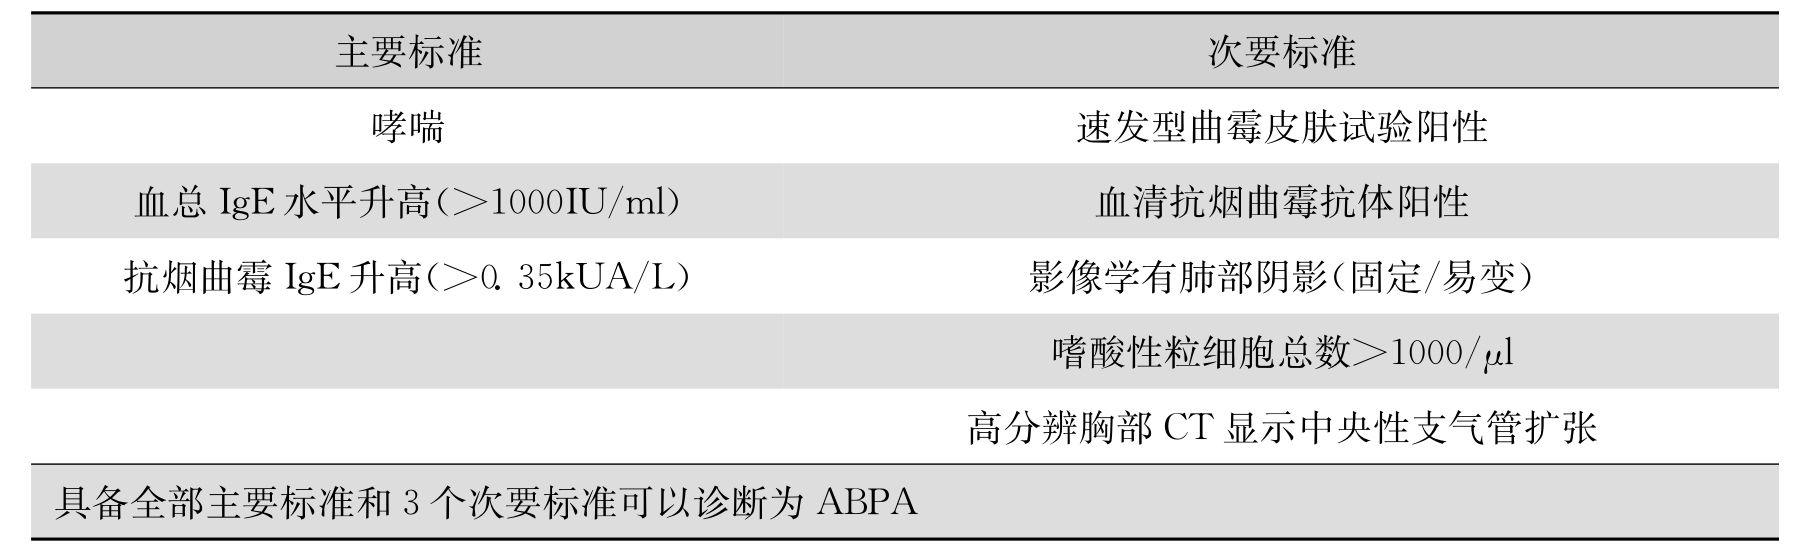
\includegraphics[width=5.97917in,height=1.84375in]{./images/Image00017.jpg}
\end{table}

诊断肺曲霉病除职业史(鸟禽饲养者、酿造工人、农业接触发霉稻谷者等)、机体免疫状态、临床表现及X线检查外,确诊有赖于组织培养及组织病理学检查,或呼吸道标本培养阳性,涂片见菌丝。血清曲霉抗体测定和血、尿、脑脊液及肺泡灌洗液曲霉半乳甘露聚糖测定和PCR测定血中曲霉DNA对本病诊断亦有帮助。变应性支气管肺曲霉病患者的诊断需与支气管哮喘相鉴别。

\paragraph{三、肺毛霉病}

肺毛霉病少见。此病常继发于糖尿病、肝硬化、结核病、恶性肿瘤、白血病及慢性感染的基础上,一般发生于终末期病变。病理改变主要为急性化脓性肺炎、多数性肺脓肿形成与肺坏疽。临床症状无特异性,主要为咳嗽、咳粉红色与黄红色痰、发热与白细胞增多。此霉可向全身播散,侵犯各脏器(心、肾、脑、肺等)。胸部影像学检查(尤其是胸部CT)可以显示单发或多发性浸润影或结节影,有时呈楔形改变,好发部位多为上叶,可双肺同时受累,下叶较少见。诊断有赖于组织病理学。

\paragraph{四、肺隐球菌病}

肺隐球菌病是由具有致病性的新生隐球菌及其变种感染引起的急性或亚急性肺真菌病,近年患病率有增加趋势。隐球菌经呼吸道侵入,在肺内形成感染灶,本病可呈急性、慢性或血源性播散,常引起隐球菌性脑膜炎。免疫抑制宿主(如AIDS)和健康人均可发病。临床分为无症状型、慢性型和急性型。急性型患者可有发热、咳嗽、咳黏液痰,盗汗、乏力和体重减轻。少数病例呈急性肺炎表现,高热、气急、低氧血症,可导致急性呼吸衰竭。以下线索诊断时可参考:①原先健康者肺部X线显示孤立或多发性结节状或块状阴影,特别是病变位于胸膜下时,常有空洞形成;毒性症状不明显;②免疫抑制患者出现肺部浸润,可单侧或双侧,可出现弥漫性间质性改变或粟粒状阴影;③肺部病变伴有脑膜炎表现者。

诊断可用痰涂片采用墨汁染色,可见圆形厚壁孢子,可有出芽现象,孢子内有反光颗粒,可提示诊断。组织活检可作最后诊断。播散型隐球菌病可做血、尿、脑脊液、皮肤损害的脓液等涂片及培养检查,阳性者可诊断。此外,乳胶凝集试验检测隐球菌荚膜多糖体抗原检测也有助诊断,非脑膜炎患者血清的阳性率为20\%~50\%。

\paragraph{五、肺孢子菌肺炎}

长期以来肺孢子菌一直被划归为原虫,但DNA研究证实肺孢子菌更接近于真菌,同源性介于子囊菌和担子菌之间。近年来核酸序列分析显示,人类与动物中分离出来的肺孢子菌差异很大。因此,国际上将从人类中检出的病原体改名为耶氏肺孢子菌(pneumocystis
jiroveci),而寄生于大鼠的则命名为卡氏肺孢子菌。同时建议保留PCP的缩写用法,但其含义改为肺孢子菌肺炎(pneumocystis
pneumonia)。肺孢子菌肺炎是免疫功能低下患者最常见以及最严重的机会感染性疾病之一。近年来发病率急剧增加,与免疫抑制剂、器官移植和艾滋病的流行有关。其感染途径主要为空气传染和体内潜伏状态肺孢子菌的激活。临床上分为流行型(经典型)与散发型(现代型)。流行型主要发生于2~6个月龄的早产儿、营养不良儿;散发型好发于免疫缺陷、肿瘤化疗、长期应用糖皮质激素或免疫抑制剂的儿童和成人。起病缓慢,早期有低热、腹泻、纳差、体重减轻,继而出现干咳、进行性呼吸困难、发绀等,常发生呼吸衰竭。体征常缺如,与症状的严重程度分离。胸部X线检查早期典型改变为双侧肺门周围弥漫性渗出,呈网状和小结节状影,然后迅速进展成双侧肺门的蝶状影,呈肺实变,可见支气管充气征。本病诊断有赖于活检组织特殊染色找到病原体。有文献报道实时定量PCR检测敏感性98\%,特异性96\%,可帮助分辨患者是否为PCP感染期。

艾滋病患者中PCP是最重要的机会感染之一,约85\%左右的晚期艾滋病患者合并PCP,25\%的艾滋病患者死于本病。近年国内报告的一组200例艾滋病患者中,已确诊PCP的有12例,其中4例合并结核病,1例合并肺炎链球菌肺炎。患者均有发热、咳嗽,干咳无痰;体温37.5~39.0℃,其中10例有呼吸急促、呼吸困难、发绀。肺部听诊2例有肺底部少许可变性湿啰音,2例少许干啰音。治疗前患者痰PCR检测均阳性,血PCR检测9例阳性;六胺银染色、吉姆萨染色找卡氏肺孢子菌分别有5例和6例阳性。

\subsubsection{3.1.8 寄生虫感染}

\paragraph{一、阿米巴肺脓肿}

阿米巴肺脓肿目前已比较少见。病变通常位于右下肺,因此病多由阿米巴肝脓肿穿破横膈至肺所引起,胸膜也同时累及。有时左叶肝脓肿向左膈穿破而引起左侧胸膜、肺阿米巴病。在少数病例中,阿米巴原虫由肠道病灶经血行传播至肺部,有些病例可无肝或肠阿米巴病病史,形成所谓“原发性肺阿米巴病”,易使人误会病变原发在肺。肺阿米巴病患者就诊时往往以发热、咳嗽、咳痰、右下胸痛与右肩放射痛为主诉,发热多为高热,弛张热型,伴或不伴寒战,可有气促、盗汗、纳差等症状。脓肿破入支气管时咳出大量酱红色或巧克力色黏稠脓性痰,对提示本病的诊断有重要意义。体检可发现肝脓肿体征。腹部B超和CT有助于诊断。

阿米巴肺脓肿的主要诊断依据是:①肠道或肝阿米巴病的病史;②大量典型的酱红色或巧克力色黏稠脓性痰,可检出溶组织阿米巴滋养体,但阳性率低于20\%;③右下肺叶病变,以及在X线透视下右膈局限性隆起与运动减弱等;④对甲硝唑(灭滴灵)治疗具有迅速而显著的疗效。疑似病例应考虑作抗阿米巴诊断性治疗。

\paragraph{二、急性血吸虫病的肺部病变}

急性血吸虫病较常并发肺部病变。肺部病变的出现距离感染期40余天至2个月左右,约2~3个月之后吸收并遗留少许痕迹。患者的临床表现有发热及其他毒血症症状等,伴有肝大压痛与外周血嗜酸性粒细胞增多。呼吸道症状大都轻微,咳嗽较常见,偶尔有咯血;胸部体征甚少,可有干、湿啰音。X线所见主要为弥漫性浸润,按其病灶显示的形态,可分为:①小斑片状阴影;②片状阴影;③大片状阴影;④粟粒状阴影等四类。

急性血吸虫病肺部病变的主要诊断根据是:①患者有急性血吸虫病的证据;②上述的肺部症状与X线征;③除外其他原因的肺部病变;④吡喹酮治疗疗效良好。

\paragraph{三、人比翼线虫病}

人比翼线虫病系罕见的疾病。自1913年发现以来,据报道全世界病例约100例。国内曾报道3例,一起进食未煮熟的鳖而致感染。主要症状为慢性阵发性咳嗽与咳黄痰,病程1个月后有血痰,体重减轻,亦可有胸痛。抗生素治疗无效是本病的特点。痰沉渣涂片检查可找到虫卵,孵化后虫壳内可见到幼虫。胸部X线表现无特殊性,大多数无异常发现,有的可表现为支气管炎或肺炎。纤维支气管镜检查所见主要表现为支气管黏膜充血,可有肉芽肿形成。特征表现是气管支气管内可见鲜红色血丝样的Y形线虫,钳出体外可见虫体蠕动。如怀疑此病可嘱患者仔细观察咳出的痰,有时可见虫体而诊断。

\protect\hypertarget{text00026.html}{}{}

\subsection{3.2 变态反应性疾病}

\subsubsection{一、单纯性肺嗜酸性粒细胞浸润症(吕弗勒综合征)}

单纯性肺嗜酸性粒细胞浸润症又称吕弗勒综合征(Löffler's
syndrome),主要特点是短暂而易消散的肺部浸润阴影,伴以短暂的外周血嗜酸性粒细胞增多。多数病例有短期的发热。参考第7.2.3节。

诊断本病的主要依据是:①病程短暂与良性经过;②发热、咳嗽、咳痰,肺部听诊可有干性或湿性啰音等症状与体征;③外周血嗜酸性粒细胞增多;④X线检查肺部有短暂性浸润阴影,呈游走性,消散后不留痕迹。

\subsubsection{二、风湿性肺炎}

风湿性肺炎少见,一般发生于风湿热的基础上。临床表现一般可区分为轻、重两型。轻型病例仅轻微咳嗽,偶有血丝痰,肺部可发现湿啰音,病变局限,可并发胸膜炎,预后较佳,因症状轻微,临床上易被忽视。重型病例病变广泛,往往突然出现脉快、心悸、气促、发绀、胸痛、咳血丝痰等症状,体温波动较大,病情较重,但肺部体征却轻微甚或缺如。X线表现多种多样,出现迅速,消散也快,有时呈游走性反复出现,连续X线检查,对临床诊断常起决定性作用。

风湿性肺炎的诊断主要根据:①有符合风湿热的临床表现;②上述的胸部症状与X线征;③除外其他原因的肺部病变,如过敏性肺炎、肺炎支原体肺炎等。抗链球菌溶血素“O”测定及C反应蛋白反应,对此病的诊断往往有帮助。

\protect\hypertarget{text00027.html}{}{}

\subsection{3.3 风湿性疾病}

许多风湿性疾病可有发热和肺部浸润。系统性红斑狼疮可有间质性或小叶性肺炎等肺部表现,常与胸膜炎并发。狼疮性肺炎表现为发热、干咳、气促,X线胸片可见片状浸润阴影,多见于双下肺。因多有白细胞减少,且抗生素治疗无效,可误诊为病毒性肺炎,但激素治疗后肺炎迅速消退。类风湿关节炎、系统性硬化病、多发性肌炎-皮肌炎等可有发热和肺部浸润病变,结节性多动脉炎的肺部病变多伴有咯血。临床上应注意鉴别,目前由于免疫学检查的普及,诊断一般不难。

\protect\hypertarget{text00028.html}{}{}

\subsection{3.4 化学性及物理性损害}

\subsubsection{一、化学性肺炎}

在化学工业生产过程中或其他原因而致吸入高度刺激性的化学性气体(如氮氧化物、硫化氢、氯、二氧化硫、汽油等),可引起急性肺部病变,表现为肺炎与急性肺水肿。

\paragraph{(一)汽油吸入性肺炎}

患者以汽车司机及其助手为多见,一般在吸入后立即发生剧烈咳嗽,并常有咯血,2~8小时后体温开始上升,大多数持续于38~39.5℃之间,最高达40℃以上。其他常见症状为胸痛、头痛、头晕、昏厥、恶心、呕吐、呼吸困难等。体检出现肺部浊音、肺泡呼吸音减弱、湿啰音等。X线检查在发病后3~6小时内,一般即可发现肺部大片密度不均匀,边缘模糊的实变阴影,后者与肺门相连,其周围有散在性、密度不甚高的斑点状阴影。此病如能及时恰当处理,一般预后良好。

\paragraph{(二)胃酸吸入性肺炎}

系胃酸反流吸入引起的化学性肺炎,亦称孟德尔森综合征(Mendelson
syndrome)。以年长者居多。临床上以胃酸反流后出现咳嗽、发热、呼吸困难为主要表现,继而出现急性呼吸窘迫综合征(ARDS)。本病国外报道较多,临床对发热、很快出现呼吸窘迫、发绀的患者,尤其是老年患者应注意鉴别。

\subsubsection{二、药物性肺病}

有些药物如呋喃妥因、青霉素、碘、复方乙酰水杨酸、异戊巴比妥等可引起变态反应性肺部病变,发病急,表现为发热、全身性皮疹、双肺湿啰音、X线胸片呈斑片状阴影等。诊断时需仔细寻找用药史。

\subsubsection{三、急性放射性肺炎}

急性放射性肺炎是由于放射线治疗胸部疾病(如支气管肺癌)所引起的一种合并症。此病发病较急,预后不良,目前尚无有效疗法。急性放射性肺炎的诊断主要根据下列各点:①病史:胸部曾接受大面积高剂量的放射治疗,发病前有感冒史;②症状:干咳、气促、微热,进行性病情加重;③体征:有发绀、呼吸困难,照射区内叩诊浊音,并可听到湿性与干性啰音;④化验检查:白细胞总数不增多;⑤肺部X线检查:照射野内有密度增高的片状或网状阴影,尤以肺门区为显著。

\protect\hypertarget{text00029.html}{}{}

\subsection{3.5 特发性间质性肺炎}

\subsubsection{一、急性间质性肺炎}

急性间质性肺炎(AIP)又称Hamman-Rich综合征,是一种病因未明、起病急骤、病情危重,以肺部弥漫性浸润并迅速发展为呼吸衰竭为特征的肺部疾病。患者起病突然、进展迅速,在较短时间内出现呼吸衰竭,平均存活时间很短,大部分在1~2个月死亡。绝大部分患者在起病初期有类似上呼吸道病毒感染的症状,半数以上的患者突然发热、干咳,伴进行性加重的呼吸困难。双肺底可闻及散在的细捻发音。实验室检查不具有特异性。X线胸片显示双肺广泛弥漫性浸润阴影。近年国内文献已有报道。本病临床表现为病情急剧进展的急性呼吸系统疾病,患者有发热、咳嗽、进行性呼吸困难乃至快速导致呼吸衰竭。X线胸片显示双肺广泛弥漫性浸润阴影。病因与发病机制尚未明了。诊断须排除各种已知原因的急性肺疾病方能确定,尤须与ARDS相鉴别,主要根据临床和病理的认真分析以及糖皮质激素的治疗效果。

\subsubsection{二、隐源性机化性肺炎}

隐源性机化性肺炎(COP),指不明原因的机化性肺炎(OP),是一种以细支气管、肺泡管、肺泡腔内肉芽组织栓形成为特征的肺部非特异性炎症过程,包括继发性机化性肺炎和隐源性机化性肺炎(COP)。后者指没有明确病因的“特发性”机化性肺炎。以往曾称为闭塞性细支气管炎伴机化性肺炎(BOOP)。该病主要表现为干咳、呼吸困难,呼吸困难多为活动后气短,程度多数较轻,部分患者可出现发热、纳差、体重下降。胸片可表现为双侧斑片状浸润影,主要分布于胸膜下及肺野外带,在病程中可有游走性。胸部CT表现分为:①多发性肺泡实变影(典型COP):多见于双肺胸膜下或沿支气管血管束分布,病变大小从几厘米到整个肺叶不等,可有支气管充气征及游走性表现。②浸润性阴影(浸润性COP):表现为双肺底网织状阴影伴磨玻璃影,浸润型由定义不清的弓形病变或小叶旁的多角形病变组成,通常伴随着其他阴影尤其是实变影。③局灶性实变影(局灶COP):局灶肺泡浸润影常位于上肺,边缘清楚,常呈叶、段分布,偶有空洞。肺部影像学具有多发性、多态性、易变性和病变多在肺外周的特点,加上抗生素治疗无效,临床诊断并不困难。糖皮质激素治疗效果一般较好。

\protect\hypertarget{text00030.html}{}{}

\section{4 周期性发热}

患者的体温突然或徐缓上升到高峰,保持数小时乃至若干天,然后迅速或徐缓下降至正常,经若干天无热期后又再发热,历数小时至若干天后又下降至正常。如此发热期与无热期互相交替,反复多次,即周期性发热。周期性发热原因可分为感染性与非感染性两类(表\ref{tab2-13})。

\begin{table}[htbp]
\centering
\caption{周期性发热的疾病分类}
\label{tab2-13}
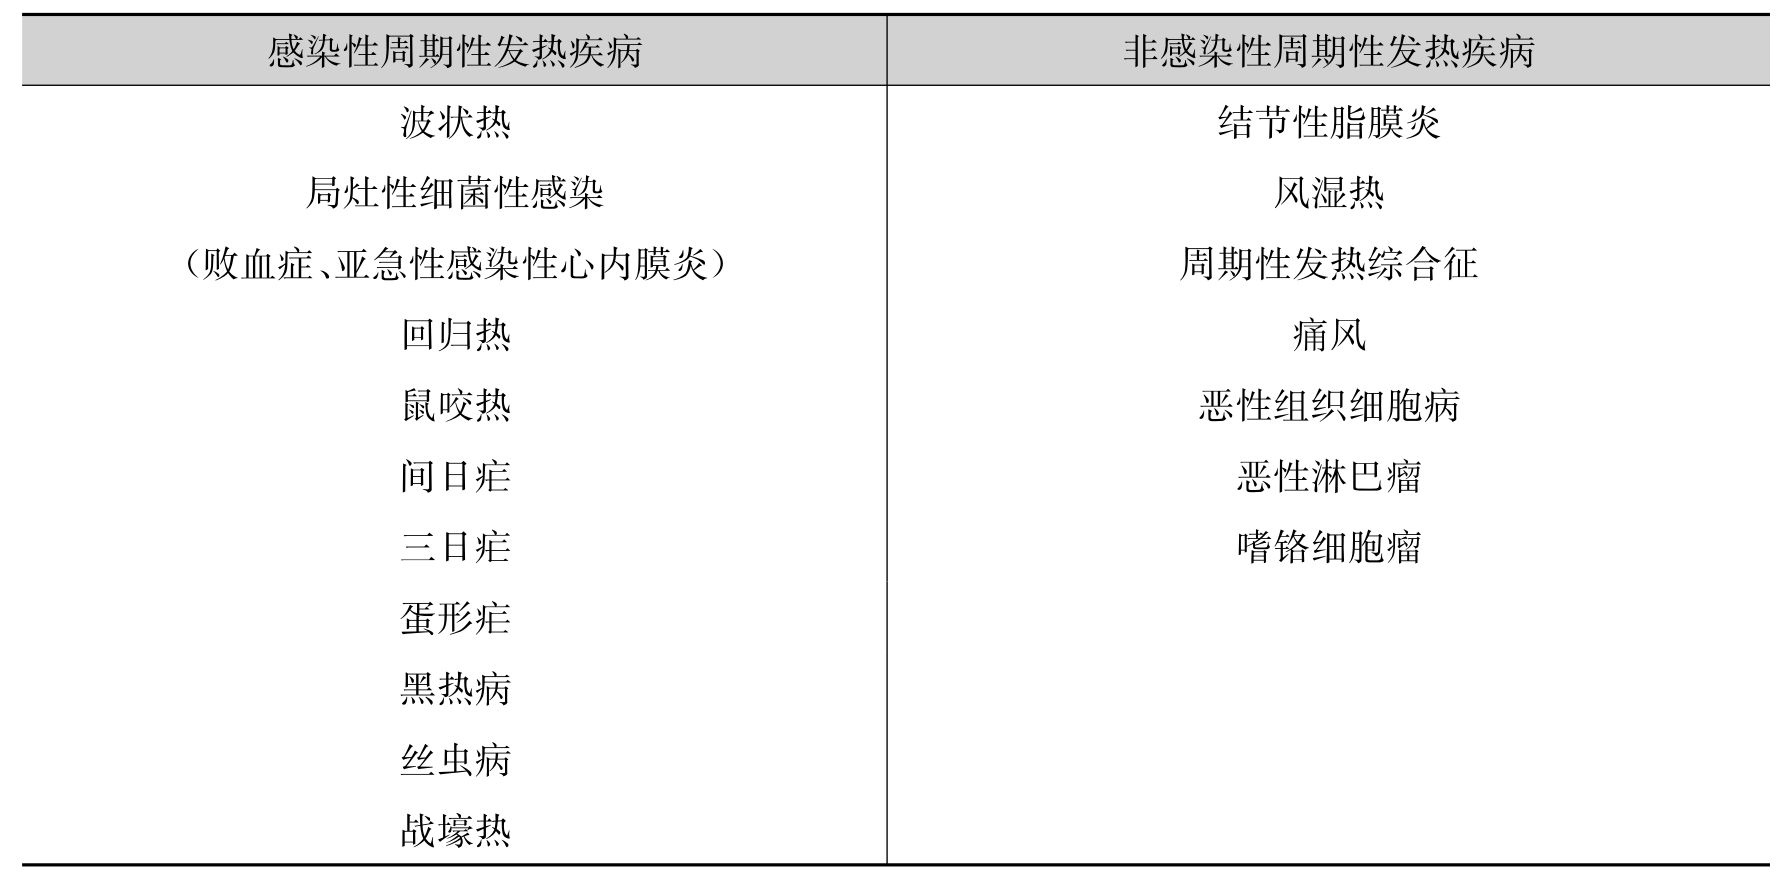
\includegraphics[width=5.92708in,height=2.9375in]{./images/Image00018.jpg}
\end{table}

\subsection{4.1 感染性周期性发热疾病}

\subsubsection{一、波状热(布鲁菌病)}

波状热的主要传染源是受感染的羊、牛与猪。文献报告约15\%~22\%病例具有典型的波状热型、每次发热期自6天至数周不等,一般有几个热波,可自行退热而进入缓解期,经数天至数周,热度又见回升。此种反复发生的周期性发热可迁延累月经年之久(参见第5.1节)。

\subsubsection{二、局灶性细菌性感染}

肾盂肾炎、支气管扩张合并感染、血栓性静脉炎、胆囊炎等部位处受到细菌性感染,都可引起反复的发热或寒战发作,但间歇期并无规则。

一侧慢性腰痛伴有原因未明的间歇性发热,除慢性复发性肾盂肾炎之外,肾结核也须考虑。国内报告不典型肾结核,可仅以间歇性发热为临床的唯一表现。

对于反复发生细菌性感染的患者,尤其是同类病原体引起的反复感染(如肺炎双球菌性肺炎),应考虑低(或无)丙种球蛋白血症或无能丙种球蛋白血症的可能。低(或无)丙种球蛋白血症可为先天性或获得性。诊断方法主要是测定血清中免疫球蛋白定量,缺乏IgG或7S丙种球蛋白时,抗细菌、抗病毒的抗体也常缺乏,致反复发生感染。无能丙种球蛋白血症与低丙种球蛋白血症不同,患者的血清蛋白电泳有高于正常或正常量的丙种球蛋白,只是表现丙种球蛋白的功能有缺陷,免疫功能低下,对各种感染有极大的易感性,人工自动免疫试验无抗体形成(如接种伤寒菌苗后,肥达反应阴性)。本症可为特发性或继发性,常继发于骨髓瘤、淋巴瘤、白血病等。

\subsubsection{三、败血症、亚急性感染性心内膜炎}

在败血症与亚急性细菌性心内膜炎病例中,有时可出现间歇性发热,类似疟疾发作,如不注意详细检查,可致误诊(参见第1.1节)。

\subsubsection{四、回归热}

回归热是由回归热螺旋体引起的急性虫媒传染病,引起人类发病者有虱传和蜱传回归热螺旋体,前者国内已罕见报道,后者散发于世界各地,我国以南疆及山西等地为主要发病地。本病特点为急起急退的高热,短期热退呈无热间歇,数日后又反复发作,发热期与间歇期交替反复出现,并有全身肌肉酸痛、肝脾大。间歇期除感虚弱外,其他症状均减退或消失,血白细胞多增高,也可正常,中性粒细胞增多。发作次数频繁者贫血严重,可有丙氨酸转氨酶升高,凝血酶原时间延长等,发热期采血涂片检出螺旋体可确诊。

回归热可分为流行性回归热与地方性回归热二型。前者以体虱为传染媒介,症状较重;后者由壁虱传播,症状较轻。

在流行性回归热多发的冬春季节及地区,如患者有寒战、高热、头痛、肌痛、鼻出血,并发现带虱或曾与此病患者有密切接触史者,须考虑此病的可能性,应作厚滴血片或血涂片镜检回归热螺旋体。

据国内报告;地方性回归热发病季节以4~8月为高,有严格的地区性,诊断地方性回归热须注意以下几点;①发病急骤.发热呈不规则的间歇型,初次发作持续时间为2~6天。以后发作仅持续数小时至一天。无热期长短不一,自1~14天,因而呈现不规则的周期性发热曲线。②症状较流行性回归热为轻。③患者无带虱现象,反之往往有被壁虱刺咬史。④血液及骨髓涂片中螺旋体数量虽稀少难找,但在无热期也可找到;动物接种易于成功。⑤青霉素治疗无效,胂剂一次疗法大都复发。

有报道:女,17岁,新疆人,周期性发热3个月,每周发热1~3次,午后发热,体温达40℃,中度贫血,血涂片检出回归热螺旋体,青霉素治疗14天,未再发热。

回归热须与钩端螺旋体病、流感、斑疹伤寒、疟疾、波状热等相区别。可依靠流行病学史、临床动态观察、病原学与血清学检查,一般困难不大。

\subsubsection{五、鼠咬热}

鼠咬热罕见。引起鼠咬热的病原体已证实有两种:一为小螺旋体,一为念珠状链杆菌。国内报告的病例大都由前者引起。由后者引起的仅属个别病例。

诊断鼠咬热首先须注意鼠咬史。由小螺旋体引起的鼠咬热有以下临床特征:潜伏期5~21天。患者通常以寒战、高热急骤发病,全身症状较重。最有诊断价值的特征是在鼠咬部位发生热、肿、痛,呈紫黑色,可形成水疱、组织坏死或硬性下疳样溃疡,上覆以黑色痂皮,并有局部淋巴结炎。发热持续数天而骤退,但经数天后又再发,呈回归热型、发热期间鼠咬伤部位炎症加剧,患者可发生皮疹,抽血作暗视野荧光检查,可发现活动迅速的小螺旋体,在皮肤损害处采取分泌物或肿胀的局部淋巴结穿刺检查,更易获得阳性结果。胂剂或青霉素治疗有效。

由念珠状链杆菌引起的鼠咬热,症状基本与上述相似,但潜伏期较短,仅1~5天,咬伤处炎症反应不显著,胂剂疗法不理想,但青霉素治疗有良效。可将患者血液作培养或接种于小白鼠腹腔内而确定诊断。

鼠咬热须与疟疾、回归热、斑疹伤寒及败血症等相鉴别,主要根据鼠咬史与病原学检查。

\subsubsection{六、间日疟}

凡在夏、秋季节,患者有周期性发冷、发热、盛汗,呈隔日发作兼有脾大与贫血,须考虑间日疟的可能性。如患者在疟区居留或最近曾到过疟区,间日疟的临床诊断大致可以成立。血涂片发现间日疟原虫是确诊的可靠依据。

在各种疟疾中,间日疟较为多见。分布也较广。潜伏期通常为10~14天,输血疟疾则较短(7~10天)。

患者以突然寒战急骤发病,颜面苍白,虽盖厚被仍未能止冷。发冷持续约1/2~2小时,继而体温迅速上升,高热往往达40~41℃。此时患者颜面转为潮红、头痛、口渴,有时谵妄;皮肤干热,脉快。发病5~7小时后开始大量出汗,持续约2~3小时衣摆尽湿,体温恢复正常或降至常温以下。整个发作过程持续6~10小时,单纯感染者每隔48小时周期发作一次。发作多在中午至下午,经数次发作后,脾脏可触及,并出现继发性贫血。有的病例出现唇疱疹,对诊断有一定意义,因唇疱疹少见于其他类型疟疾。

典型间日疟的临床诊断较易,但二重感染者、混合感染者(常见是间日疟合并恶性疟)以及曾接受不规则抗疟治疗者症状常不典型,易误诊为其他急性发热疾病。此时作厚滴血片或血涂片镜检疟原虫是确定诊断的最简捷方法。如厚滴血片阴性,必要时可作骨髓穿刺涂片检查。口服氯喹作诊断性治疗可用于高度疑似的病例。

\subsubsection{七、三日疟}

三日疟比较少见,大多为散发性。病初发热不高,呈不规则型、弛张型热,3~5天后较为典型发作,症状与间日疟相似。有发冷、发热及出汗阶段,但每隔72小时发作一次,且多在午后发作。单纯感染者发作周期经常不变。发作数次后出现脾大与贫血。

三日疟的临床诊断可根据典型的周期性发作、脾大与继发性贫血。二重感染者可每发作二天间歇一天,三重感染者可每天发作,因而必须注意与其他发热性疾病相鉴别。血涂片镜检发现三日疟原虫是诊断的最可靠依据。

\subsubsection{八、蛋形疟}

蛋形疟是最少见的疟疾,流行季节为4~7月和10~12月。蛋形疟的发作周期与间日疟同,也为48小时,但其发作常在黄昏或晚间。临床症状轻重不一,轻症者可无明显症状,重症者发热可达41℃或以上,并可持续十余小时之久,甚至发生谵语。此病在治愈后不易复发。确诊须依靠从血液中检出蛋形疟原虫。

\subsubsection{九、黑热病}

有些黑热病患者的早期症状与波状热相似,体温曲线呈波状起伏,并有大量出汗,脾大与白细胞减少。这种情况甚至使人不会想到黑热病。偶尔早期患者的血清可凝集布鲁菌,但滴度不超过1∶160。另一方面,有时早期黑热病的症状可酷似间日疟,但血片镜检疟原虫始终阴性,抗疟治疗无效。

黑热病的诊断须根据流行病学史、临床表现与骨髓穿刺检查。

\subsubsection{十、丝虫病}

丝虫病患者发作丝虫热时,通常在剧烈运动或疲劳之后,突以畏寒或寒战而起病。继而体温急骤上升,可达40℃,伴淋巴管(结)炎,持续1~3天而消退,但也可持续达一周之久。往往每隔2~4周或数月发作一次。

\subsubsection{十一、战壕热(五日热)}

战壕热可以每隔五天出现寒热发作为特征,并有皮疹,腰、腿肌痛与胫骨痛,病程长短不一。此病是一种立克次体感染,传染媒介为体虱,国内未发现。

\subsubsection{十二、其 他}

偶见有钩虫病致周期性发热3个月,间歇3~4天发热1次,持续3~4小时自退,患者有嗜酸细胞增多,贫血,大便隐血弱阳性,粪找虫卵阴性。胃镜发现十二指肠降部数条钩虫。

\protect\hypertarget{text00031.html}{}{}

\subsection{4.2 非感染性周期性发热疾病}

\subsubsection{一、结节性脂膜炎}

结节性脂膜炎(Weber-Christian病)是一种原发于脂肪小叶的非化脓性炎症,是较少见的一种变态反应性疾病。好发于青壮年女性。根据受累部位,可分为皮肤型和系统型。

临床表现以反复全身不适、关节痛、发热、皮下结节为特征,受累的皮肤反复发生红斑,时有压痛,并有水肿性皮下结节,损害呈多发性、对称性、成群分布、最常受累的部位是双下肢,常伴全身不适,发热与关节疼痛,亦可出现恶心、呕吐、腹痛、体重下降、肝脾大及其他内脏损害,其病程有很大差异,主要取决于受累器官的情况,内脏受累广泛者,可出现多脏器功能衰竭、大出血或并发感染。

结节性脂膜炎发热的特点:半数以上皮肤型发热可为低热、中度热或高热,热型多为间歇热或不规则热,少数为弛张热,通常在皮下结节出现数日后开始发热,持续时间不定,多在1~2周后逐渐下降;系统型的发热一般较为特殊,常与皮疹出现相平行,多为弛张热,皮疹出现后热度逐渐上升,可高达40℃,持续1~2周后逐渐下降。

实验室检查多为非特异性改变,白细胞总数可正常、增多或减少,血沉快。皮肤结节活检的组织病理学改变是诊断的主要依据。

此病可被误诊为败血症、伤寒、肺结核、颈淋巴结结核、风湿热、结节性红斑、恶性组织细胞病等。凡有发热及皮下结节的病例疑似此病时,应及时作结节活检明确诊断。

\subsubsection{二、风湿热}

风湿热有复发的倾向。

\subsubsection{三、周期性发热综合征}

周期性发热综合征是非常罕见的疾病,作此诊断时必须慎重考虑,患者自幼年即可起病,偶见于成年人,每隔数天、数周或数月发作一次。间歇期患者俨如常人,因间歇期近于规则,有时可推测其发作日期。

周期性发热综合征(PFS),具有下列共同特征:①复发性和周期性发热;②发热持续时间大多相同,少则2~8日,多则2~4周,比一般的原因不明发热时间短;③多系统炎症(滑膜、浆膜及(或)眼、皮肤等炎症表现);④自限性;⑤实验检查中急性期反应物显著升高,但始终查不到感染性病原,迄今也未查到任何自身免疫疾病的特征;⑥在无症状间歇期患者可完全正常。吲哚美辛或糖皮质激素治疗能迅速解热。

目前按照间歇期的不同形式作为分型基础:①无热间歇期固定的PFS包括周期性中性粒细胞减少症,PFAPA综合征;②无热间歇期不固定而有所变异的PFS(高IgD综合征等);③缺乏无热间歇期的PFS。

国内曾报告个别周期热病例,患者发热期间伴有关节酸痛、皮疹。白细胞增多、血沉加快等表现,反复发作周期热,各项检查均无特殊发现,未接受任何治疗,发热周期自行停止,随访22年未能弄清病因。

\subsubsection{四、痛 风}

痛风每次发作时可伴有发热。

\subsubsection{五、恶性组织细胞病}

此病偶尔可以周期性发冷发热、多汗为主要表现。

\subsubsection{六、恶性淋巴瘤}

恶性淋巴瘤易引起发热,文献报告可达31\%~50\%,且可以发热为初发症状,而此时尚无其他明显的临床表现。热型种类不一,而回归型热(周期热)约见于1/6的霍奇金淋巴瘤,具有一定的特征性。每一发热周期持续2~4周不等。

周期性发热而无浅表淋巴结肿大的恶性淋巴瘤,病变通常位于腹腔、腹膜后、纵隔等处的淋巴结或结外病变,诊断常有困难,须与其他原因的周期性发热疾病相区别。患者常有多汗、疲乏、消瘦或相应结外病变的表现,根据深部淋巴结或结外病变的部位行病灶活检方能确诊。

有报道女,51岁,周期热4年,每次发热伴有咳嗽、咳痰,抗生素治疗效果欠佳,胸部CT显示右肺中叶及左肺下叶实变,误为肺炎,后支气管镜检查肺活检示肺黏膜相关淋巴组织型边缘区B细胞淋巴瘤。提示少数非霍奇金淋巴瘤患者也可表现为周期性发热。

\subsubsection{七、嗜铬细胞瘤}

嗜铬细胞瘤的主要表现是高血压。高血压多为阵发性,发作时可伴有体温升高、头痛、出汗等表现。国内曾有个别病例报告,以突发性间歇性发热住院多次,并疑为疟疾,最后经详细检查方证实为嗜铬细胞瘤。

\protect\hypertarget{text00032.html}{}{}

\section{5 长期发热}

长期不明原因发热(FUO)是指发热持续3周以上,体温≥38.5℃,经完整的病史询问、体格检查及常规实验室检查后仍不能明确诊断者。这类患者的临床表现不典型或病情不呈典型临床经过;或临床医生对某些少见疾病或病变认识不足;某些疾病的病灶隐蔽,不易为常规检查手段所发现等因素所致难以明确发热的病因。

国外对特殊人群的FUO有着特别的定义:

\subsection{1.人类免疫缺陷病毒(HIV)阳性者}

体温≥38.3℃超过4周,其中住院患者热程超过3日仍不能明确病因即可诊断。

\subsection{2.粒细胞缺乏者}

外周粒细胞计数<0.5×10\textsuperscript{9}
/L,体温≥38.3℃超过3日,培养阴性2日以上。

\subsection{3.老年患者}

除病者为老年人外,其他标准同经典的FUO。

\subsection{4.住院患者}

因非感染性疾病而入院的患者,发热超过3天病因不能明确者。

长期发热的热型可以多种多样;但以弛张热及不规则热等热型为多见。热程长短对FUO诊断具较大的参考价值。一般来讲,热程短,有乏力、寒战等中毒症状者,有利于感染性疾病的诊断;如热程中等,但呈渐进性消耗、衰竭者,以肿瘤多见;热程长,无毒血症症状,但发作与缓解交替出现,则有利于结缔组织病的诊断。

可引起FUO的病因超过200种,长期发热的原因是复杂的,除中枢性原因外,可概括为以下四大类(表\ref{tab2-14}):

\begin{longtable}{c}
 \caption{长期发热疾病}
 \label{tab2-14}
 \endfirsthead
 \caption[]{长期发热疾病}
 \endhead
 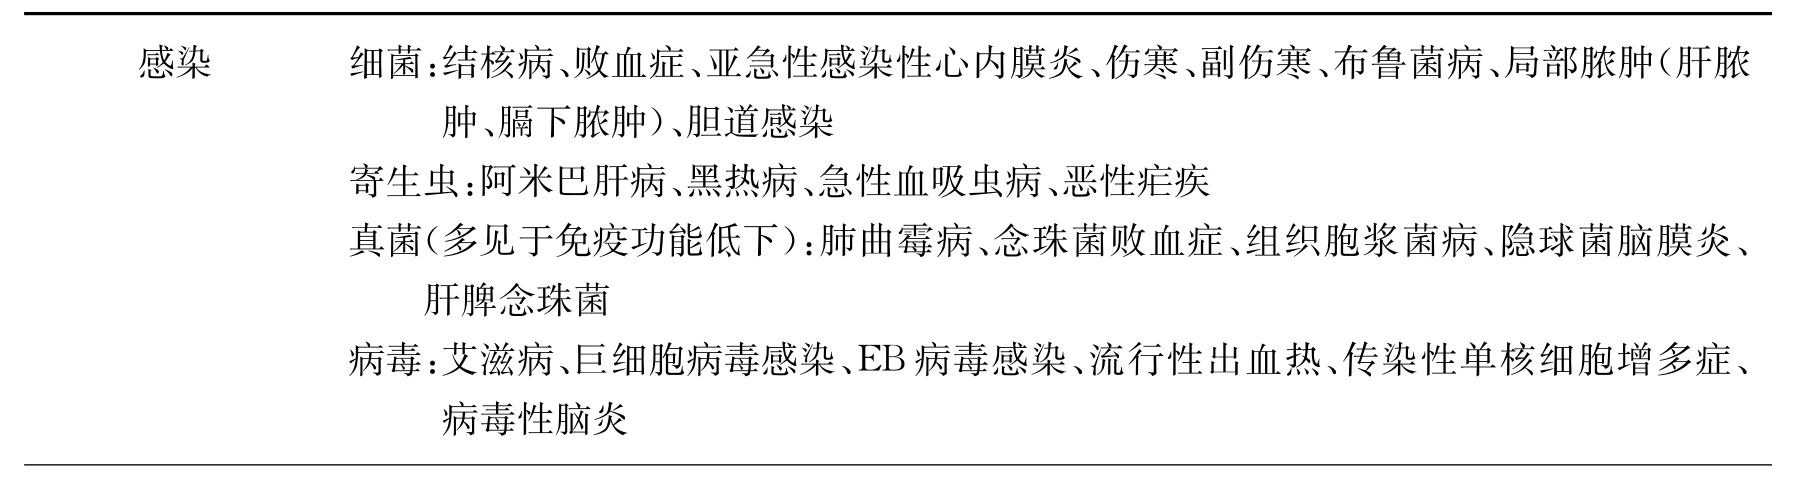
\includegraphics[width=\textwidth,height=\textheight,keepaspectratio]{./images/Image00019.jpg}\\
 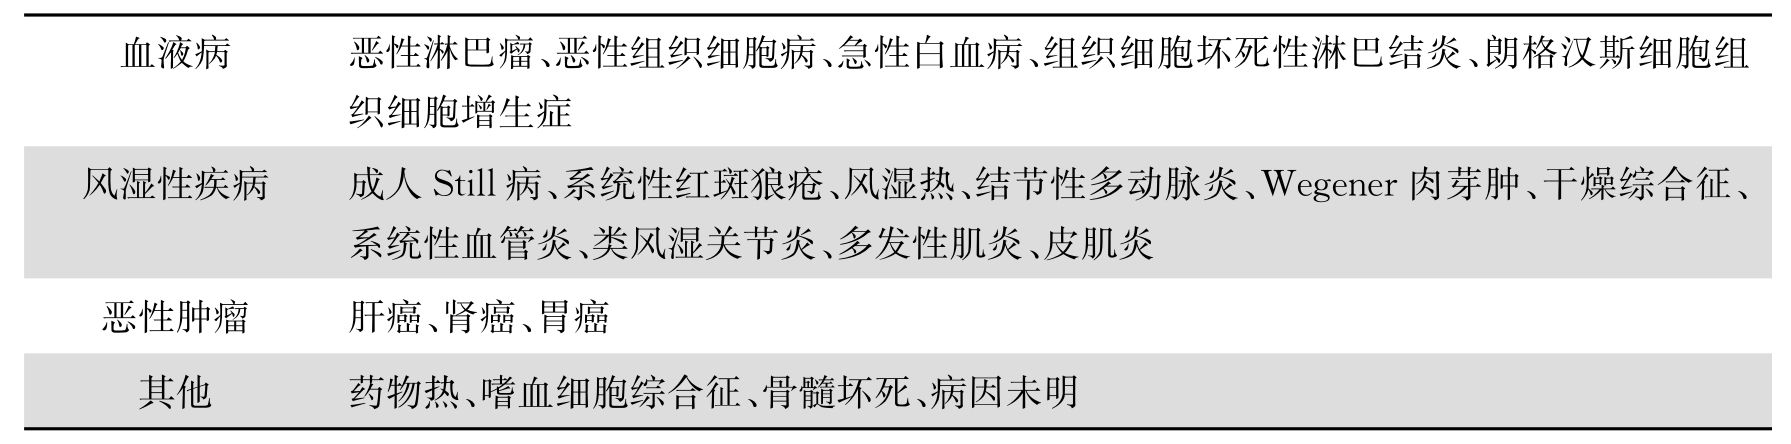
\includegraphics[width=\textwidth,height=\textheight,keepaspectratio]{./images/Image00020.jpg}
 \end{longtable}

\subsection{一、感 染}

感染是长期发热最常见的原因。在各种感染中,结核病是主要原因之一,特别是某些肺外结核,如深部淋巴结结核、肝、脾结核尤难于诊断;早期的急性粟粒型结核和脊椎结核也难于诊断。

其他感染还有伤寒与副伤寒、亚急性感染性心内膜炎、布鲁菌病、败血症、阿米巴肝病、CMV病毒、HIV、真菌等。

\subsection{二、血液病}

不明原因发热中以淋巴瘤所占比例最高,常成为诊断难题。

发热、出血、进行性贫血,肝、脾、淋巴结肿大,可提示血液病诊断的线索。

\subsection{三、风湿性疾病}

风湿性疾病的临床表现多种多样,其中,发热可以为首发症状,亦可在病程中出现。有报道各种风湿性疾病出现发热的几率排列为:Still病100\%,SLE
70\%~80\%,干燥综合征20\%,肌炎及(或)皮肌炎10\%,系统性硬皮症约5\%。其中Still病约占结缔组织病发热的50\%。临床上两个以上互不相关的器官损害表现可提供结缔组织病的诊断线索,其中以多发性关节炎与皮疹是最常见的共同表现,且往往早期出现,还可出现心、血管、肝、肾、肺、肌肉等器官和组织的损害。其实验室检查的特点是自身抗体及高免疫蛋白血症。

\subsection{四、恶性肿瘤}

恶性肿瘤生长迅速,当肿瘤组织崩溃或合并感染时则可引起长期发热。如肝癌、结肠癌,早期易漏诊。血清乳酸脱氢酶活性、癌胚抗原(CEA)、甲胎蛋白(AFP)等测定有助于诊断。

李龙芸回顾了1953-1997年《中华内科杂志》刊出的124例病例的临床病理(例)讨论见表\ref{tab2-15}及表\ref{tab2-16},确诊方法:尸检85例,开胸探查5例,开腹探查11例,组织活检15例及实验室检查8例。疑难发热病病因以感染性、血液系统及肿瘤疾病为主,分别为36.4\%、30.2\%及20.9\%。感染性疾病中以细菌性及结核性感染为主,其次为病毒性、寄生虫性及霉菌性感染。血液性疾病中以淋巴瘤、恶性组织细胞病为主。结核性疾病及寄生虫感染无减少趋向,病毒及霉菌性感染报道增多,尤其艾滋病、卡氏肺孢子菌肺炎及巨细胞病毒。对疑难发热病例应警惕结核、细菌性感染及寄生虫、淋巴瘤、恶性组织细胞病、恶性肿瘤等。这组患者结核病以中青年为主,热程1~18个月,平均(6.1±5.7)个月。淋巴瘤大多数热程超过1年。恶性组织细胞病10天~3年,平均(6.2±5.7)个月。成人Still病热程1个月~1年,平均5.3个月。

1998-2013年《中华内科杂志》刊出长期不明发热的临床病例讨论29例的病因见表\ref{tab2-17},29例中淋巴瘤占45\%。

\begin{table}[htbp]
\centering
\caption{1953-1997年《中华内科杂志》刊出的47例疑难临床病理讨论的感染性疾病发热的病因}
\label{tab2-15}
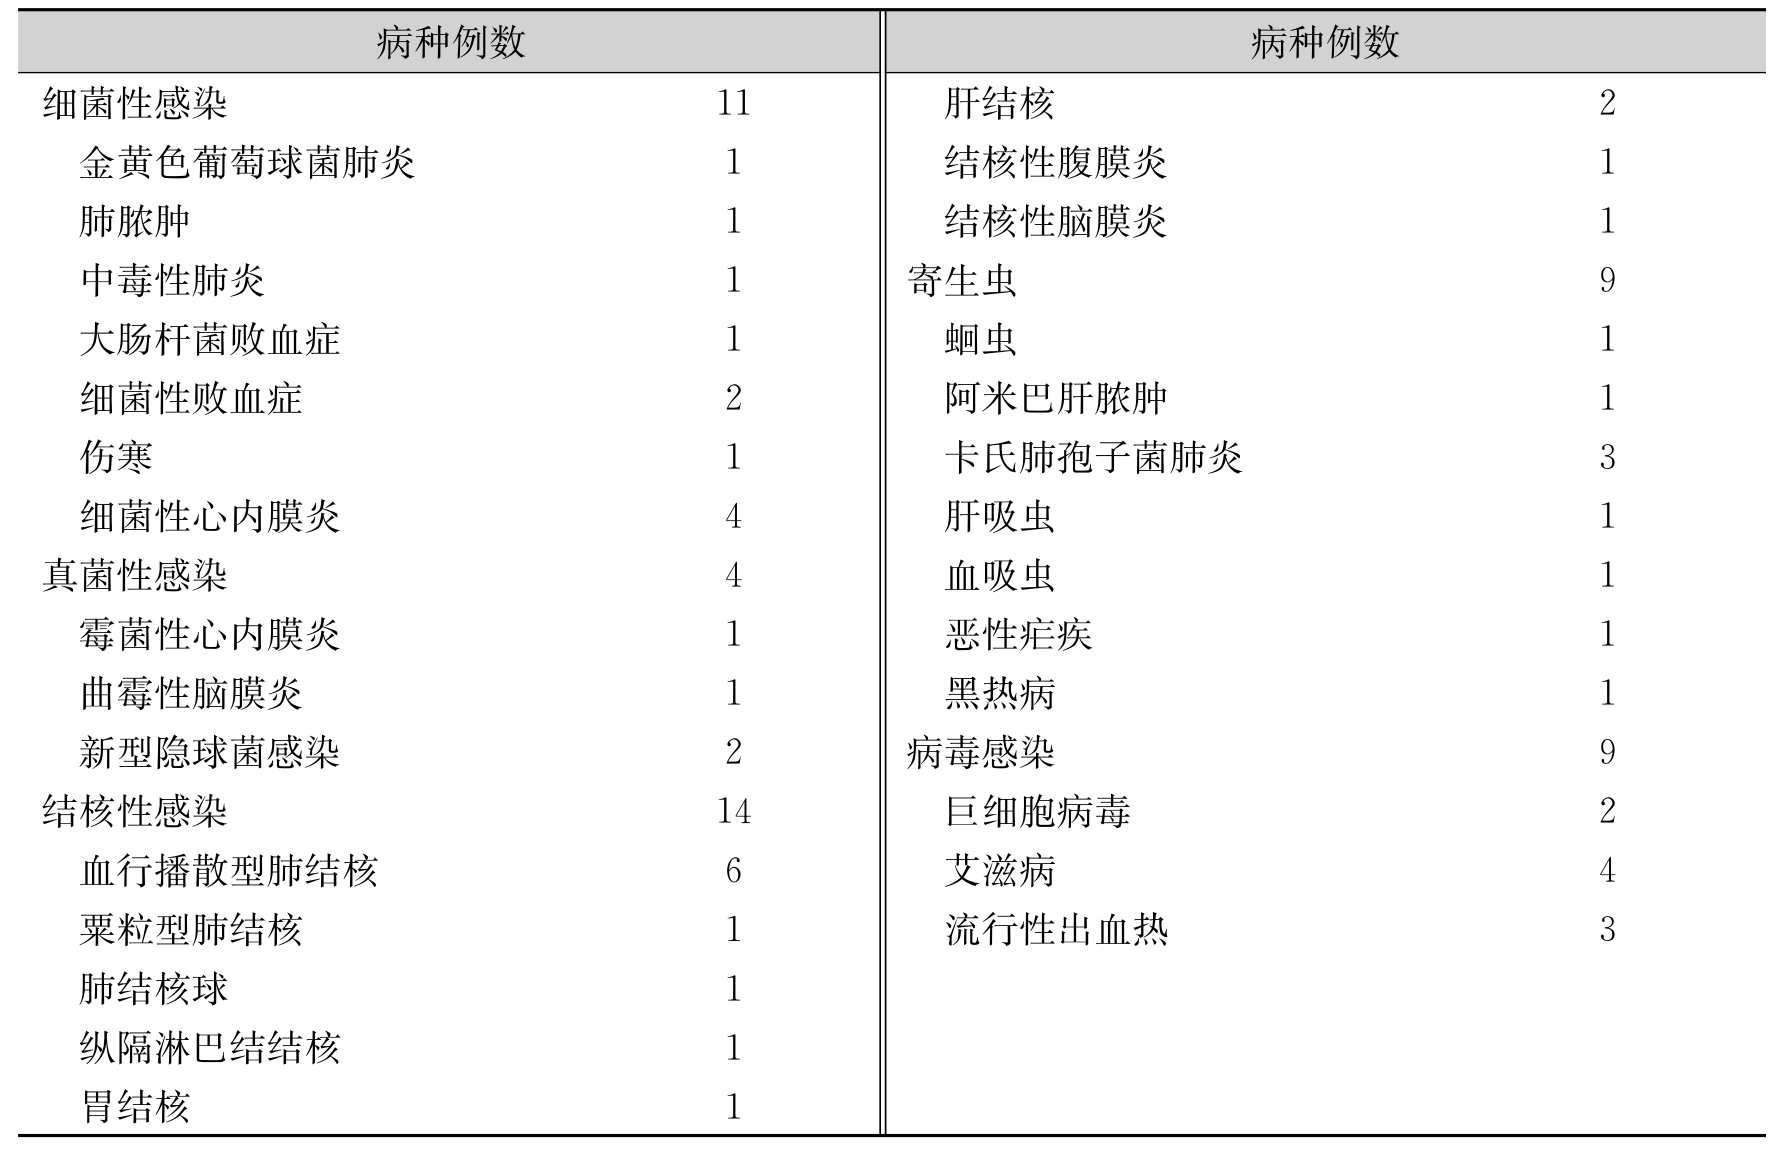
\includegraphics[width=5.94792in,height=3.83333in]{./images/Image00021.jpg}
\end{table}

\begin{table}[htbp]
\centering
\caption{1953-1997年《中华内科杂志》刊出发热疑难临床病理讨论的肿瘤、血液、结缔组织病性疾病}
\label{tab2-16}
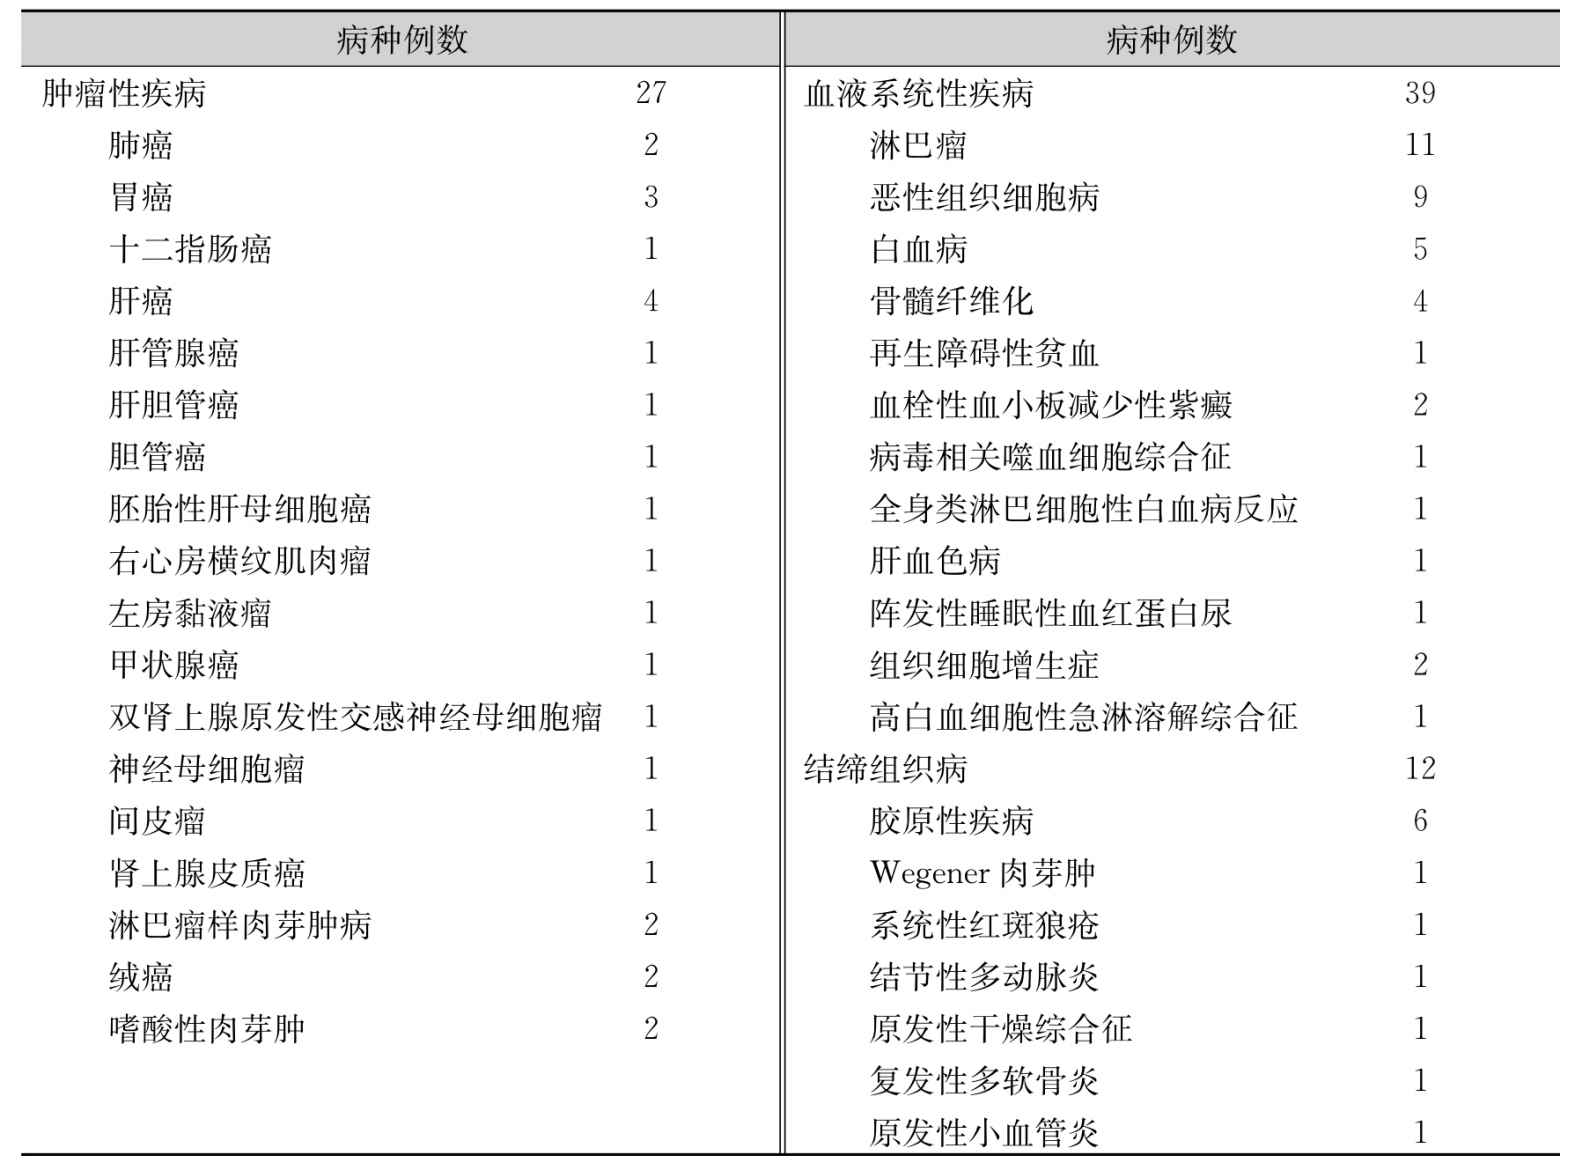
\includegraphics[width=5.95833in,height=4.41667in]{./images/Image00022.jpg}
\end{table}

\begin{table}[htbp]
\centering
\caption{1998-2013年《中华内科杂志》刊出长期不明发热的临床病例讨论29例的病因}
\label{tab2-17}
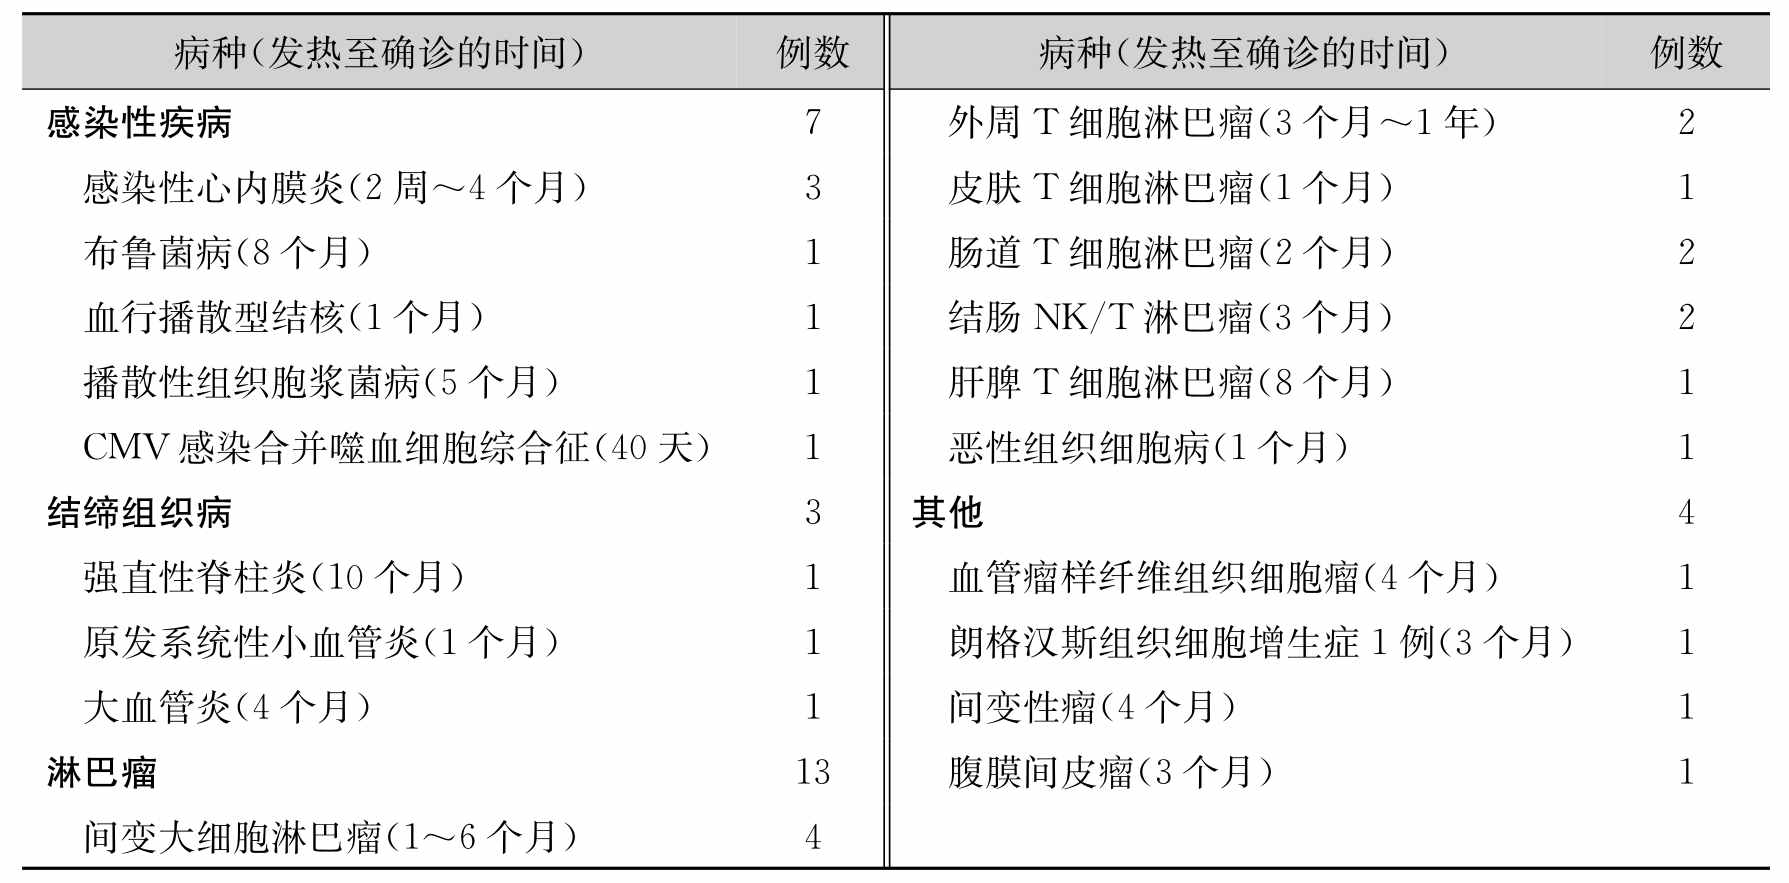
\includegraphics[width=5.95833in,height=2.92708in]{./images/Image00023.jpg}
\end{table}

另有报道一组未明原因长期发热449例(表\ref{tab2-18})。病因包括:感染性疾病(56.8\%),其中结核病占43.6\%;且以肺外结核居多,肺外结核临床表现复杂多样,但大多数患者除长期发热外,常伴乏力、纳差、盗汗、消瘦等结核中毒症状,随着病情进展,有些可出现结核感染部位的症状,也可有血沉增快、γ-球蛋白比值升高、结核菌纯蛋白衍生物(PPD)阳性。一般抗生素治疗无效,需特异性抗结核治疗才有效。PPD强阳性有助于结核病的诊断,但其阴性也不能除外结核诊断。本组有1例腰椎结核患者在院外误诊达15个月之久,故需提高对肺外结核的认识。

此组疾病中结缔组织病19.6\%,其中成人Still病34.6\%,是结缔组织病中引起长期不明原因发热的主要病因。

肿瘤性疾病16.5\%,其中淋巴瘤39.1\%;诊断最困难,因此如怀疑本病建议多次行淋巴结活检,局限于上消化道的淋巴瘤可做胃镜及活检,腹腔内淋巴瘤必要时手术探查,尽早明确诊断,及时治疗。

其他疾病7.1\%,其中坏死性淋巴结炎占33.3\%,药物热占26\%;出院时仍未确诊13.8\%。

\protect\hypertarget{text00033.html}{}{}

\subsection{5.1 感染性疾病}

\subsubsection{一、结核病}

结核病是感染性疾病中引起不明原因长期发热的主要原因。马小军等在2004年的研究显示,449例FUO患者中结核病占21.4\%。侍效春等报道不明原因发热为表现的100例结核病中,可以中高度发热,热型以不规则热为多见,弛张热、稽留热次之,39\%患者有寒战,热程3~77周,中位热程为12周。结核累及部位:单纯肺结核39例,单纯肺外结核28例包括腹腔结核(肠结核、结核性腹膜炎、肝结核、腹腔淋巴结结核)11例、淋巴结(颈部、腹股沟、纵隔)结核4例、结核性心包炎2例、结核性脑膜炎2例及无明确部位9例,肺结核合并肺外结核33例,50\%患者PPD皮试阳性,实验室检查多为ESR增快和C反应蛋白升高以及不同程度的消耗表现即贫血和低白蛋白血症,诊断方法:抗酸杆菌阳性的34例,组织病理符合结核病的8例,临床诊断并经抗结核治疗有效的49例,诊断性抗结核治疗有效的9例。接受抗结核治疗后显效的时间平均为5.3周。从发病至确诊的时间为3~77周,中位确诊时间14周。诊断性抗结核治疗依旧是目前诊断肺外结核的主要方法。对结核病高度可疑病例的诊断性抗结核治疗观察时间放宽到8周,较广为采用的期限4~6周为宜。

\begin{table}[htbp]
\centering
\caption{449例不明原因长期发热的病因分类}
\label{tab2-18}
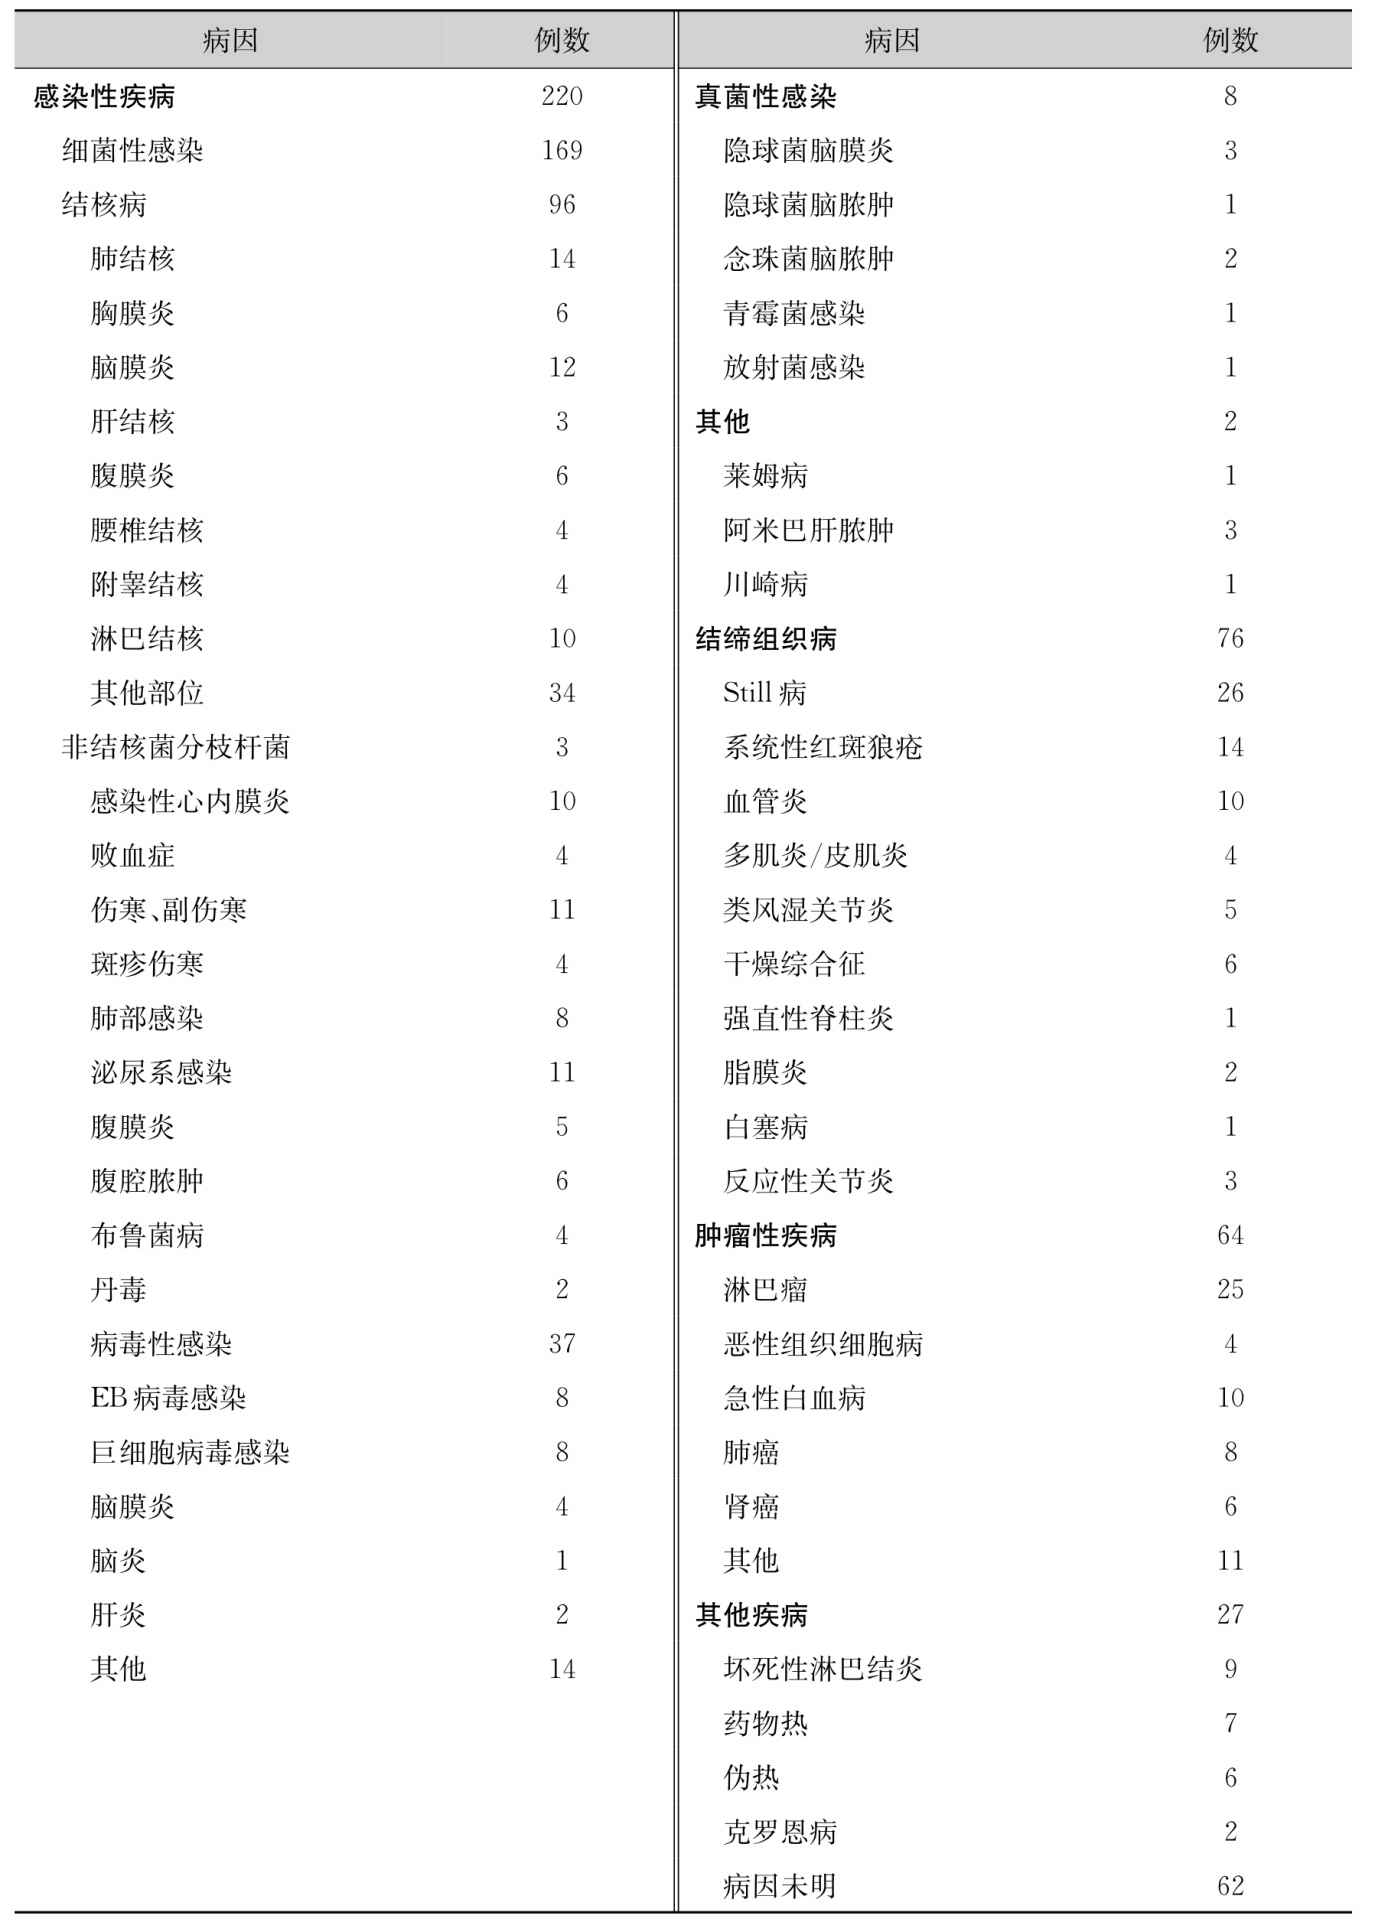
\includegraphics[width=5.97917in,height=8.40625in]{./images/Image00024.jpg}
\end{table}

\paragraph{(一)急性粟粒型肺结核}

过分相信X线胸部透视的阴性结果,可能漏诊急性粟粒型肺结核。易致漏诊或误诊为伤寒型粟粒型肺结核。一个类似伤寒的患者,而有脉快、呼吸迫促、轻度发绀、血象白细胞减少(但也可增多)兼有淋巴细胞减少,体格检查未发现明显的心肺体征,应考虑急性粟粒型肺结核的可能性。此病以儿童及青年人为多见,但中年以上也可罹患。虽然一次胸部照片阴性,对怀疑病例需隔1~2周再作胸片复查。

\paragraph{(二)肝结核}

肝结核的患者大多数存在肝外结核病灶,部分可以没有肝外病灶。在血源性播散时结核杆菌经肝动脉而进入肝脏,若继发于胃肠道结核病灶则可经门静脉系统而进入肝脏。肝结核临床上少见,由于缺乏典型症状,诊断较为困难,在未确诊之前临床表现不易与淋巴瘤相鉴别。

值得注意的是所谓“原发性”肝粟粒性结核,此病一般常规检查难以发现其他结核病灶。此种病例甚为罕见,诊断极困难。国外文献提到“原发性”肝粟粒性结核的下列诊断依据可供参考:①原因未明的发热;②肝大,不一定伴有压痛;③脾大;④关节痛或皮疹;⑤腹部胀满而躯体消瘦;⑥腹水的蛋白含量高于4g\%;⑦未能解释的血沉加快、中等度贫血与白细胞减少;⑧未能解释的血清球蛋白增加;⑨阳性的结核菌素试验。患者大多具有上述表现的大部分或全部。此病多见于青壮年人,发热可迁延甚久。CT肝扫描可发现肝粟粒病灶,确诊须依靠肝穿刺活检。笔者见女性,60岁,反复中高发热9个月,全血细胞减少,总胆红素104μmol/L,结合胆红素79μmol/L,非结合胆红素25μmol/L,转氨酶升高,纤维蛋白原低,凝血酶时间延长,胸片示右肺尖少许陈旧性结核,PPD皮试阴性,腹部CT:肝不大,脾稍大,在B超引导下进行肝穿刺活检,考虑为(肝脏)结核,经抗结核治疗好转出院。

\paragraph{(三)脾结核}

多见于青壮年,表现为长期发热、弛张热、左上腹不适、脾大,可无脾外结核表现,结核菌素试验不一定阳性,B超或CT示脾内多发或单发低密度灶,CT增强后病灶无强化。不易与脾型淋巴瘤鉴别,唯有病理检查有助诊断。可行B超引导下脾穿刺活检或脾切除术。

\paragraph{(四)深部淋巴结结核}

需注意肠系膜淋巴结结核。此病多侵犯儿童与青少年,但中年以上偶患。主要症状是长期发热、与饮食无关的腹部钝痛、消瘦、盗汗等。如有肠粘连,可引起剧烈的肠绞痛。热型为弛张型或不规则型,体温可高达39℃以上,但也可为微热。血沉常明显加快,也无蔷薇疹与脾大。在病程经过中有时触及淋巴结团块,CT检查有时误诊为腹部淋巴瘤或腹腔内其他恶性肿瘤。腹部平片可发现肠系膜淋巴结钙化影像。B超引导下包块穿刺或腹腔镜检查取淋巴结活检对诊断有很大的帮助,若无条件做检查,如患者有结核病接触史或伴有其他器官的结核病,宜试行抗结核治疗,从疗效上证实对结核病的臆断;如诊断性治疗无效,可考虑剖腹探查。

其他:无反应性结核常见于器官移植术后或严重免疫抑制患者。笔者见1例无反应性结核,患急性淋巴细胞白血病行异基因干细胞移植6个月后出现长期高热,伴有血性胸水或血性心包积液,肺部无结核表现,结核菌素试验阴性,未找到结核杆菌,血象白细胞升高达(70~80)×
10\textsuperscript{9} /L,继而下降至1×10\textsuperscript{9}
/L以下,血小板≤20×10\textsuperscript{9}
/L,中、重度贫血。骨髓呈大量中性中幼粒细胞类白血病反应。这种患者试验性抗结核治疗往往作为结核鉴别诊断的方法之一。

\subsubsection{二、感染性心内膜炎}

感染性心内膜炎是长期不明原因发热的病因之一,对于长期不明发热患者,需要询问既往有无器质心脏病,并仔细听诊心脏杂音,发热若有心脏杂音、周围动脉栓塞、皮肤黏膜瘀点、贫血、脾大、应考虑本病的可能,也有缺乏心脏杂音如感染累及心脏右侧杂音,易被漏诊。超声心动图及血培养可帮助诊断。但约有7\%~28\%的感染心内膜炎血培养阴性,可能由于之前多已应用抗生素;培养方法不当;特殊感染如立克次体、真菌。心内膜炎的诊断标准见第1.1.2节中“感染性心内膜炎”部分。

近年来由于某些诊疗技术的应用增多,如漂浮导管放置时间太长、血液透析、静脉高营养治疗和静脉吸毒等,致感染性心内膜炎发病有所增加,国内报道致病菌以草绿色链球菌为多,长期用药者则以金黄色葡萄球菌为常见,其次为铜绿假单胞菌(绿脓杆菌),也有的为真菌。

\subsubsection{三、败血症}

败血症也是长期发热的常见原因之一。国内报道病原以金黄色葡萄球菌最多,大肠杆菌次之,其他细菌少见。败血症消除后患者仍可能有发热。此类长期发热原因最多为迁徙性化脓病灶,可位于体内任何组织和器官。有的深在病灶,须用影像学检查(如B超、CT)以证明之。其次为所谓“后继热”,有认为与感染消除后,体温调节中枢功能尚未稳定有关,一般为微热,少数为药物热,多伴有药疹,停用有关药物后体温复常。

\subsubsection{四、伤寒、副伤寒}

伤寒、副伤寒甲常为长期不明发热原因之一,造成诊断困难的原因是伤寒患者缺乏中毒症状,相对缓脉、典型皮疹、肥达反应缺乏特异性,也易出现阴性。

\subsubsection{五、获得性免疫缺陷综合征(艾滋病)}

由人类免疫缺陷病毒(HIV)引起,一旦进入AIDS期,常见症状有发热、咳嗽、咳痰、气短、低氧血症、乏力、消瘦、全身淋巴结肿大,反复肺和肠道感染,抗感染无效。有些患者贫血、白细胞减少、血小板减少,可以两系或三系减少。与肺间质纤维化、结节病、结核有时难以鉴别,要反复测定HIV抗体,一旦阳性,应进一步作蛋白印迹法以确证是否HIV感染。

\subsubsection{六、其他病毒性疾病}

病毒性疾病一般病程自限,EB病毒和巨细胞病毒感染可作为长期发热的病因,诊断主要依据为分离到病毒,或血清学相应抗原或特异性IgM抗体检测。虽有自限性的特点但病程迁延(5~8周),血白细胞变化特点是计数轻微升高或正常而淋巴细胞比例显著增加,有肝功能异常等多脏器受累的表现,严重者甚至出现横纹肌溶解、肾功能异常。

\subsubsection{七、侵袭性真菌病}

恶性肿瘤患者放疗、化疗后中性粒细胞减少;器官移植或免疫性疾病需要长期使用糖皮质激素或免疫抑制剂;ICU患者、HIV感染者、反复使用广谱抗生素者、慢性消耗性疾病等,上述患者出现长期发热应想到真菌感染的可能。主要致病菌有念珠菌、曲霉、隐球菌、毛霉等。曲霉病的发病有上升趋势。感染部位有内脏感染:肺、肝、脾、脑、肾、组织;全身播散:真菌败血症,其中侵袭性肺曲霉病最常见。真菌感染患者除了发热外,局部症状不明显,不及时治疗死亡率高。对于存在真菌感染高危因素的患者出现不明原因发热,需行胸部CT检查;体液(痰、尿、血)真菌培养,血培养受多种因素影响,阳性率低;葡聚糖检测(G试验)、半乳甘露聚糖抗原检测(GM试验);确诊需要侵入性的组织活检,但在状况很差的患者难实施,所以确诊困难,大多数属于临床拟诊或临床诊断。往往需要试验性治疗。血液系统恶性肿瘤患者若粒细胞减少(≤0.5×10\textsuperscript{9}
/L),不明原因发热(体温>38℃),96小时广谱抗生素治疗无效时,可进行经验性使用伏立康唑或伊曲康唑、棘白菌素如卡泊芬净、米卡芬净抗真菌治疗。

组织胞浆菌病 是一种较少见的由荚膜组织胞浆菌引起的深部真菌感染性疾病。局限性感染可无临床症状或表现为亚临床型,播散型组织胞浆菌病可累及单核巨噬细胞系统及全身脏器,如肝、脾、骨髓、淋巴结等。当吸入本菌的孢子,进入肺泡,被巨噬细胞吞噬,再通过网状内皮系统进行全身播散。疾病的严重程度取决于吸入孢子量及宿主自身免疫反应。播散型常见于长期使用糖皮质激素等免疫功能低下者,临床表现为长期高热,肝、脾、淋巴结肿大,全血细胞减少,肝酶尤其ALP升高常见。涉及胃肠道感染的可以表现为腹泻及腹痛,部分可合并噬血细胞综合征。重症者可以合并DIC,急性肾衰;易误诊为淋巴瘤、结核病。

确定诊断需做真菌检查:①骨髓涂片:可见巨噬细胞内大量卵圆形吞噬体,紫红色半月形胞质集中在吞噬体的一端,外周围绕未染色的空晕,形似荚膜。②真菌培养:通常所需时间为4~6周,形态学上具有结节大孢子是组织胞浆菌的特征。镜下组织胞浆菌典型形态为2~4μm椭圆形芽生酵母,以能被亚甲胺银染色及过碘酸-schiff(pas)染色为特征,当为进行播散型组织胞浆菌时,可在血液细胞中发现其孢子。③组织胞浆菌多糖抗原检测往往在尿液、体液中检测,在播散型组织胞浆菌中起着快速诊断作用,但容易产生假阳性,特别注意与芽生菌鉴别。组织胞浆菌需与马尔尼菲青霉菌、黑热病鉴别。

\subsubsection{八、布鲁菌病}

布鲁菌病(Brucellosis,布病),也称波状热,是由布氏杆菌引起的急性或慢性人畜共患性传染病,此病在国内多见于内蒙古、东北、西北等牧区,牧民、兽医、屠宰工人和炊事员的发病率较高。非疫区偶也有报道。饮用污染乳品也可引起感染。

布鲁菌病临床表现缺乏特异性,发热可以持续数日乃至数周以上,多数为高热、多汗、关节痛、疲乏、睾丸炎、淋巴结与肝脾大,部分患者有贫血、轻度白细胞减少,红细胞沉降率加快。实验室检查:①血液或骨髓培养:分离到布氏杆菌;②血清学检查:虎红凝集试验,试管凝集试验阳性;凝集反应通常于病期第一周后开始出现,但也可较晚,滴度在1∶100以上方有诊断价值,1∶200~400为阳性,1∶800以上为强阳性。如滴度过低,应隔一周或更长时间复查。有的病例滴度可不高,甚至呈阴性反应。血清凝集反应阴性的病例,血及骨髓培养均可出现阳性(分别为33.3\%与57.1\%)。羊型波状热病例的血培养与骨髓培养阳性率甚高(80\%)。因此如在流行疫区临床表现符合而血清凝集反应阴性,不能轻易除外此病的可能性。左氧氟沙星、利福平、多西环素抗感染有效,疗程需达6周。

布鲁菌病由于发病率低,有时接触史不明显,全身症状无特异,不易引起临床医师的重视,易导致漏诊和误诊。非疫区若饮用污染乳品出现长期不明原因发热,需做培养、血清学检查排除该病。

\subsubsection{九、阿米巴肝病}

阿米巴肝病,早期难于诊断,也易于漏诊。另一方面由于抗生素(红霉素、四环素族)的广泛应用于一般感染性发热疾病,也可使阿米巴肝病呈较为缓和的经过,而易于忽略。因此,患者有长期原因未明的发热、肝大、血象白细胞数轻度或中等度增多,不论有无肝区疼痛和过去有无痢疾史,必须考虑此病的可能性(参见有关章节)。

\subsubsection{十、黑热病}

黑热病即内脏利什曼病,是由杜氏利什曼原虫引起、通过白蛉传播的慢性地方性传染病,黑热病有严格的地区性。本病在新中国成立以来经多年大力防治,已基本消灭。近年来,甘肃、四川、新疆、内蒙古及山西等地区出现散发病例,随着经济与人员流动的全球化趋势,地方性传染病病例可能在一些传统理论中的非流行区出现,即在非疫源性地区,也偶见有散发病例报道,实验室检验人员对利什曼原虫形态不熟悉,易被误诊或漏诊。

该病各年龄均可发病,可表现为长期不明原因发热,早期病例约1/3呈双峰热型,可有畏寒,寒战,肝脾大,少数有巨脾、全血细胞减少、消瘦、进行性衰竭,骨髓易见组织细胞,在非疫区的医院就诊,易误诊为恶性组织细胞病,淋巴瘤。该病葡萄糖酸锑钠治疗有效。

对于患者长期发热原因未明而兼有肝脾大、血细胞减少等,需仔细追问是否去过疫区,须注意罕见病黑热病的可能性。黑热病的确诊须依靠以下的实验室检查:①血免疫层析试条(rK39dipstick)法检测:血清黑热病抗体阳性。②寻找黑热病原虫:骨髓穿刺发现黑热病原虫是最确实的诊断方法。在不同部位进行反复的骨髓穿刺,累积的阳性率颇高。瑞氏染色形态需与组织胞浆菌病、马尔尼菲青霉菌病鉴别,黑热病糖原染色胞内容物为红色,而后两者胞内容物不着色。

\subsubsection{十一、人粒细胞无形体病}

急性不明原因发热需注意罕见病、新发现的立克次体传染病,人粒细胞无形体病(human
granulocyticanapasmosis,HGA),是由嗜吞噬细胞无形体引起的一种经蜱传播的立克次体病,1992年在美国明尼苏达州发现HGA,且多为个例或散发流行,HGA是一种以粒细胞为主要靶细胞,常累及全身多个脏器,临床表现多样且凶险的疾病。近几年在我国江苏、湖北、河南、安徽等曾有类似疫情发生的病例报道。

HGA潜伏期一般为7~14日(平均9日),常急性起病,主要表现为不明原因发热(多为持续性高热,可高达40℃以上)、乏力、头痛、肌肉酸痛,约一半患者有消化道症状等。部分患者伴有咳嗽、咽痛,可出现意识障碍。体检可见表情淡漠,相对缓脉,少数患者可有浅表淋巴结肿大及皮疹。严重者可出现感染中毒性休克、肝炎、心肌炎、急性肾衰竭、呼吸窘迫综合征、弥散性血管内凝血(DIC)及多脏器功能衰竭等。

该病的诊断主要依据:①流行病学史:发病前2周内有被蜱叮咬或接触暴露史;在有蜱活动的丘陵、山区(林区)工作或生活史;或直接接触过危重患者的体液等。②临床表现:急性起病,主要症状为发热(多为持续性高热,可高达40℃以上)、全身不适、乏力、头痛、肌肉酸痛,以及恶心、呕吐、厌食、腹泻等。个别重症病例可出现皮肤瘀斑、出血,伴多脏器损伤、DIC等。③实验室检查:早期外周血白细胞、血小板降低,严重者呈进行性减少,异形淋巴细胞增多;外周血涂片瑞士染色镜检中性粒细胞内可见桑葚状包涵体;ALT/AST升高。急性期血清间接免疫荧光抗体(IFA)检测嗜吞噬细胞无形体IgM抗体阳性(抗体滴度≥1∶256)或急性期与恢复期双份血清IgG抗体呈4倍升高。全血或血细胞标本PCR检测嗜吞噬细胞无形体特异性核酸阳性,或分离到病原体。该病首选强力霉素治疗,有禁忌证者可选用利福平或喹诺酮类。

\protect\hypertarget{text00034.html}{}{}

\subsection{5.2 血液病}

淋巴瘤是引起长期不明原因发热最常见的恶性肿瘤。

\subsubsection{一、恶性淋巴瘤}

恶性淋巴瘤是恶性肿瘤性长期不明原因发热的主要病因,占首位(50\%)。恶性淋巴瘤是一组起源于淋巴结或其他淋巴组织的恶性肿瘤,可发生于人体内任何器官与组织,病理类型在我国以非霍奇金淋巴瘤(NHL)居大多数,霍奇金淋巴瘤(HL)仅占8\%~11\%。

以长期发热为主要和首发表现的淋巴瘤常见,临床表现复杂,尤其对那些浅表淋巴结无肿大,病灶在深部淋巴组织器官的淋巴瘤(原发于胃肠道、肺、肝、脾、骨髓、多浆膜腔、中枢神经系统、脊柱等任一部位病变),易误诊。结外病变有:①胃肠道以小肠为多,其次为胃,结肠很少受累。②胸部以肺门及纵隔受累最多,半数有肺部浸润或(及)胸腔积液。③肝、脾大。④骨髓累及者约占1/3~2/3。⑤骨骼以胸椎及腰椎最常见,股骨、肋骨、骨盆及头颅次之。⑥皮肤受累表现为肿块、皮下结节、斑块、溃疡等。⑦其他部位如鼻咽、乳腺、甲状腺、眼眶、肾上腺、肾脏、睾丸、中枢神经系统、生殖系统等均有可能受累。

淋巴瘤发热特点:

(1)发生率:淋巴瘤以发热为主要或首发症状者约占16\%~30\%,霍奇金淋巴瘤在病程早期有发热表现者可占30\%~50\%,非霍奇金淋巴瘤(NHL)约占24\%左右。NHL在病变较广泛或深部病变时更易有发热表现,侵犯到骨髓的NHL
80\%的患者均有发热表现。

(2)热型:约1/6的霍奇金淋巴瘤出现周期性热。NHL的热型呈弛张热、周期热或不规则热。

(3)热程长:有些病例待明确诊断,病程已达数月甚至达1年以上。有报道53例不明原因发热为首发的淋巴瘤,从发病到确诊的平均时间为35(5~184)周,其中大于1年病程10例。

(4)有的毒血症的表现常不明显。

(5)T-NHL比B-NHL更易有发热,有文献报道中、高度恶性T-NHL的发热为77.5\%,而B-NHL为22.4\%,尤其是皮下脂膜炎样T淋巴瘤、NK/T细胞淋巴瘤、肝脾γ/δT细胞淋巴瘤、血管免疫母细胞型T细胞淋巴瘤和间变性大细胞型(CD30\textsuperscript{+}
)淋巴瘤或称Ki-1\textsuperscript{+}
淋巴瘤、淋巴瘤性的噬血细胞综合征这些特殊类型多见有发热。

(6)抗感染治疗无效,部分应用糖皮质激素,体温可降至正常,也有用糖皮质激素无法退热。

(7)有些病例至晚期才出现肝、脾大、腹腔淋巴结肿大,白细胞减少、贫血或全血细胞减少。

对于长期不明原因发热而不能以感染性疾病、结缔组织病解释者,X线、B超、CT、MRI及正电子发射型断层扫描技术(PET)等寻找体内肿大的淋巴结和病变,尤其PET-CT对以长期发热为主要表现的淋巴瘤的筛查有价值,可以显示病灶及代谢异常,对穿刺活组织检查有定位价值;有报道的15个(723例患者)关于淋巴瘤PET
FDG显像结果进行总结,PET
FDG显像的敏感性为71\%~100\%,特异性为69\%~100\%,阴性预测值80\%~100\%。需要注意不同亚型的淋巴瘤阳性检出率不同,对弥漫性大B细胞淋巴瘤(DLBCL)、套细胞淋巴瘤(MCL)和滤泡性淋巴瘤(FL)等常见的亚型阳性检出率较高,而对淋巴结边缘区淋巴瘤(MZL)、黏膜相关性淋巴瘤(MALL型)、结外边缘区B细胞淋巴瘤(MALT-MZL)、外周T细胞淋巴瘤和伯基特淋巴瘤(BL)等少见的亚型阳性检出率相对较低。即肿瘤太小、恶性程度低等,PET-CT检查可表现为假阴性。

病理组织学和免疫组化是确诊淋巴瘤的主要依据,所以要千方百计寻找可供活检的病灶及早进行病理检查。①有浅表淋巴结肿大者,尽量选择有意义的完整淋巴结进行活组织结构及细胞形态学的检查,通过活检很容易确诊;对较深部位的淋巴结可在B超或CT引导下经皮细针穿刺活检,淋巴结病变并非弥漫分布,必要时需多次重复活检。②对于以结外病变为主要表现的淋巴瘤,根据相应病灶部位进行组织活检。③对于长期发热、肝脾大、全血细胞减少的患者,需要反复多部位骨髓活检;骨髓流式细胞仪免疫学检查、单克隆性基因重排,如免疫球蛋白重链(IgH)基因重排和T细胞受体(TCR)基因重排对诊断有一定帮助;经过多次骨髓涂片和骨髓活检后,诊断仍不明确,在无禁忌证时,腹腔镜下或剖腹行脾切除等对淋巴瘤的诊断有极大帮助。许多临床病理讨论均为淋巴瘤,说明以FUO为首发表现的淋巴瘤仍是诊断难题。

不明原因发热为首发的淋巴瘤需与成人Still病相鉴别,对于不明原因长期发热,PET-CT无显示淋巴结及结外病灶及高代谢,排除感染性疾病、肿瘤性疾病,中小量糖皮质激素或消炎镇痛药能退热者,成人斯蒂尔病可能性大。但仍需追踪排除发展为淋巴瘤。

不明原因发热为首发的淋巴瘤也需与肺外结核相鉴别。

\subsubsection{二、恶性组织细胞病}

恶性组织细胞病(简称恶组)是异常组织细胞增生所致的恶性疾病。过去曾采用许多不同的名称,如恶性组织细胞病、网状细胞白血病。过去报道的恶组实际上大多为伴噬血细胞综合征的恶性淋巴瘤,欧美大多数为间变性大细胞淋巴瘤,而在亚洲地区多为外周NK/T细胞淋巴瘤。真正的恶性组织细胞病极少见。此病的主要表现是高热,肝、脾、淋巴结肿大,全血细胞减少及进行性衰竭,病情凶险,预后不良。

根据恶性组织细胞浸润部位的不同,临床可有不同的表现,因此临床表现多种多样:①起病急,反复发热,持续时间可达27天至4个半月以上、全身进行性衰竭。热型以不规则高热居多(38.7\%),其次为稽留热(26.3\%)、弛张热(21.72)、间歇热(10.8\%)及低热少见(3\%),血培养始终阴性,各种抗生素治疗无效,对肾上腺皮质激素类药物反应差,即使体温有下降,常不能降至正常或下降后短期又上升,且连续应用逐渐失效。②造血系统受累的表现有出血、贫血、感染,肝、脾、淋巴结肿大。可有黄疸、肝功能损害等。③其他系统浸润的表现,如多发性浆膜腔积液,皮肤、胃肠、肺、肾、神经系统浸润引起的相应临床表现。

实验室检查:

1.血象 全血细胞减少,为本病的突出表现之一。

2.骨髓细胞形态及(或)活体组织病理学检查
是诊断本病的重要依据,骨髓涂片可检出异常的组织细胞,这些细胞占有核细胞的10\%~60\%。此病的异常细胞有五种类型:①异常组织细胞;②淋巴样组织细胞;③多核巨细胞;④单核样组织细胞;⑤吞噬细胞。异常组织细胞及(或)多核巨噬组织细胞有特异性诊断价值。由于骨髓损害可能为非弥漫性,或因骨髓穿刺取材甚少或取材欠佳,只能反映很小的局部情况,故阴性时不能除外本病的存在。必要时可在不同部位穿刺检查。有些病例骨髓穿刺涂片阴性,却在尸检骨髓组织切片中发现异常组织细胞。其他部位活体组织病理检查,可行皮肤、淋巴结、肝脏、脾、骨髓活检。目前缺乏识别组织细胞的特异性抗体,通常组织化学染色显示溶菌酶染色阳性,抗胰蛋白酶阳性,α1-抗胰糜蛋白酶阳性,CD68\textsuperscript{+}
为组织细胞的标志。

对不明原因的长期发热而不能以感染性疾病解释者,尤其是伴有全血细胞减少和肝、脾、淋巴结肿大,应考虑本病可能性。结合骨髓或活体组织病理学检查找到异常组织细胞及(或)多核巨噬组织细胞,同时排除反应性组织细胞增多症和Ki-1阳性的T细胞淋巴瘤,可以确立诊断。恶性组织细胞病需与下列疾病鉴别:

1.反应性组织细胞增多症
某些疾病(例如伤寒、结核病、败血症、结缔组织病等),有时骨髓涂片检查可以有组织细胞明显增多,这种反应性组织细胞增多症与恶性组织细胞病的鉴别对治疗和预后都有极为重要的意义,但二者的鉴别有时颇为困难,表\ref{tab2-19}可供参考。

2.CD30\textsuperscript{+}
的间变性大细胞型淋巴瘤(Ki-1阳性的T细胞淋巴瘤,ALCL) 占成人NHL
的3\%,本病与恶性组织细胞病在临床上、组织病理上易发生混淆,前者从分子水平证实其属T细胞系。45\%的患者有t(2;5)(p23;q35)染色体易位;CD30阳性;60\%~85\%的患者可检测出间变性淋巴瘤激酶基因(ALK)阳性;大部分病例CD2\textsuperscript{+}
、CD4\textsuperscript{+}
、细胞毒相关抗原TIA-1、颗粒酶B阳性,而呈CD3\textsuperscript{-}
、CD5\textsuperscript{-} 、CD7\textsuperscript{-} 。而恶组则无相应改变。

\begin{table}[htbp]
\centering
\caption{反应性组织细胞增多症与恶性组织细胞病的鉴别}
\label{tab2-19}
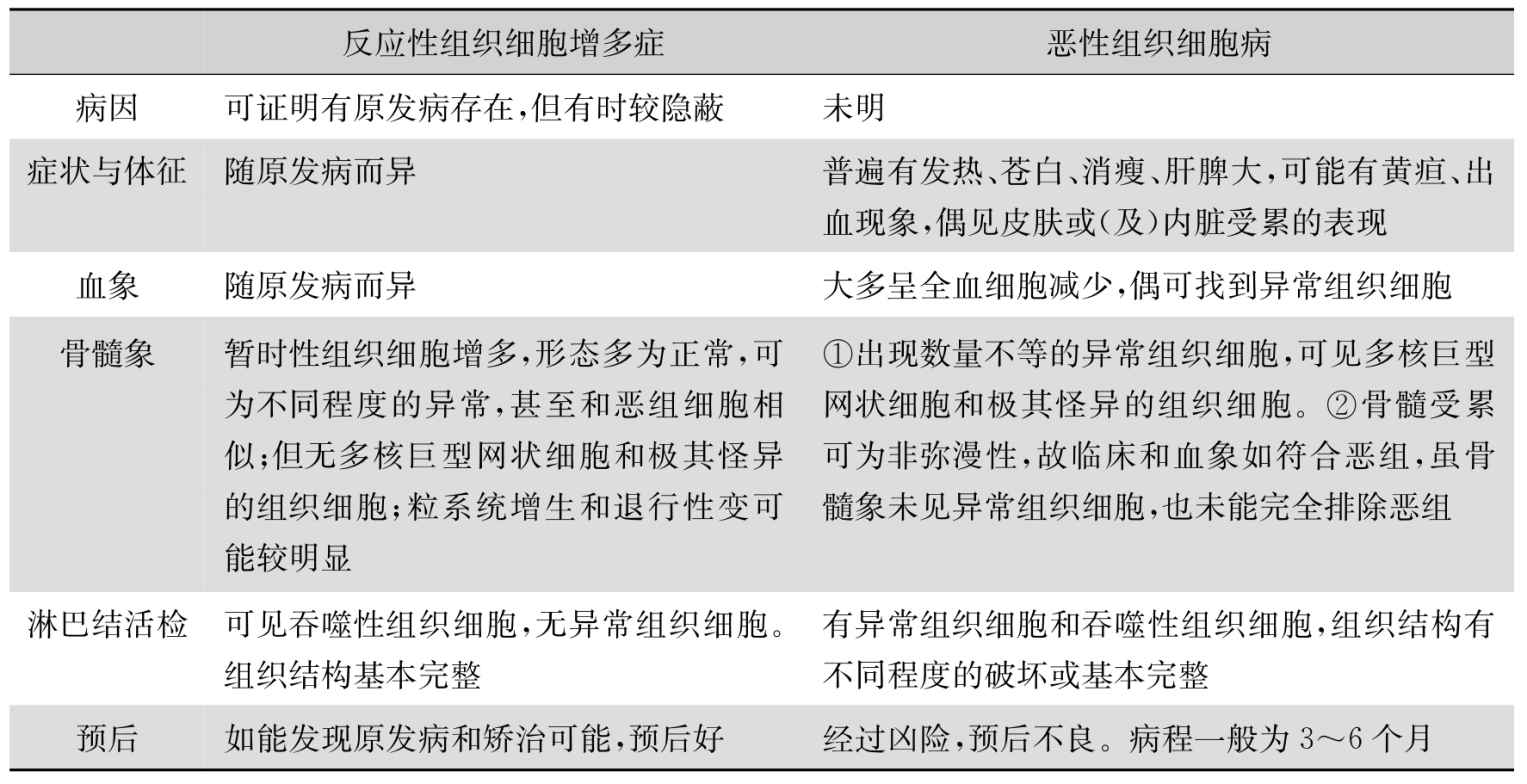
\includegraphics[width=5.90625in,height=3.02083in]{./images/Image00025.jpg}
\end{table}

\subsubsection{三、噬血细胞综合征(HPS)}

噬血细胞综合征是单核/巨噬系统反应性疾病,以组织细胞良性、大量增生,伴有明显的吞噬血细胞现象为特征。噬血综合征常常难以查出其病因,长期高热是噬血细胞综合征之一的表现,是由T细胞、巨噬细胞活化分泌IL-1、IL-6等内源性致热原而引起发热。

2004年国际组织细胞协会噬血细胞综合征的诊断标准:①发热,持续7天以上,体温超过38℃;②脾大;③全血细胞减少;④高甘油三酯血症或低纤维蛋白血症;⑤骨髓、脾、淋巴结中可见到吞噬红细胞、粒细胞或血小板的组织细胞;⑥NK细胞活性减低或缺失;⑦铁蛋白升高(铁蛋白≥3SD正常值,通常≥1000ng/ml);⑧可溶性IL-2受体(sCD\textsubscript{25}
)水平明显升高。8项中符合5项可考虑噬血细胞综合征。分遗传性和获得性,前者常发生于0~2岁的婴幼儿,后者可继发于感染(病毒尤其EB病毒、细菌、真菌、原虫)、淋巴瘤和自身免疫性疾病。其中EB病毒感染相关的噬血细胞综合征是长期不明发热的病因之一,包括EB病毒阳性的T淋巴细胞增殖症和淋巴瘤相关的噬血细胞综合征,前者血清EBV抗体滴度增高、EBDNA拷贝数升高,但淋巴结病理检查中未见典型的淋巴瘤表现,骨髓细胞也未检出克隆性T细胞受体重排。后者早期常常难以诊断,随病情进展组织活检有淋巴瘤的依据。

\subsubsection{四、急性白血病}

半数的患者以发热为早期表现。可低热,也可高达39~40℃以上,伴有畏寒、出汗等。外周血象初时有的仅有白细胞升高,红细胞、血小板数正常,易被考虑为感染性疾病。但动态观察红细胞、血小板可进行性下降。有的患者有不同程度的白血病细胞增殖浸润的表现如淋巴结肿大,肝、脾大、胸骨下段压痛,骨、关节疼痛,牙龈增生、肿胀,皮肤结节、斑块,中枢神经系统浸润的表现,睾丸浸润。血象:大多数患者白细胞增多,也有白血病数正常或减少,分类可见数量不等的原始及(或)幼稚细胞,有不同程度的正细胞性贫血,绝大多数患者血小板减少,常低于<20×10\textsuperscript{9}
/L。骨髓象是诊断急性白血病的主要依据。急性白血病患者的骨髓白血病性的原始细胞占骨髓有核细胞≥20\%。因此,凡遇有原因未明的发热伴有进行性贫血、出血者应行骨髓穿刺涂片检查以确诊。

有的患者血象呈全血细胞减少,无肝、脾、淋巴结肿大,需与急性再生障碍性贫血相鉴别。有的患者表现以出血为主,临床可与特发性血小板减少性紫癜相似,但后者以血小板减少为主,红细胞(出血严重者例外)与白细胞数不减少。

白细胞增多性急性白血病需与类白血病反应相鉴别(表\ref{tab2-20})。类白血病反应是机体受到较严重的病理损害时所发生的造血组织异常反应,其特征是外周血中白细胞数增多或(及)出现幼稚细胞,血象与白血病相似。病因以急性感染为多,其次为恶性肿瘤、急性溶血、中毒、大出血、结核病、寄生虫病等,按细胞类型可区分为中性粒细胞型、淋巴细胞型、单核细胞型、嗜酸性粒细胞型等。病因去除后类白血病反应即消除,有助于诊断。

\begin{table}[htbp]
\centering
\caption{类白血病反应与急性白血病鉴别}
\label{tab2-20}
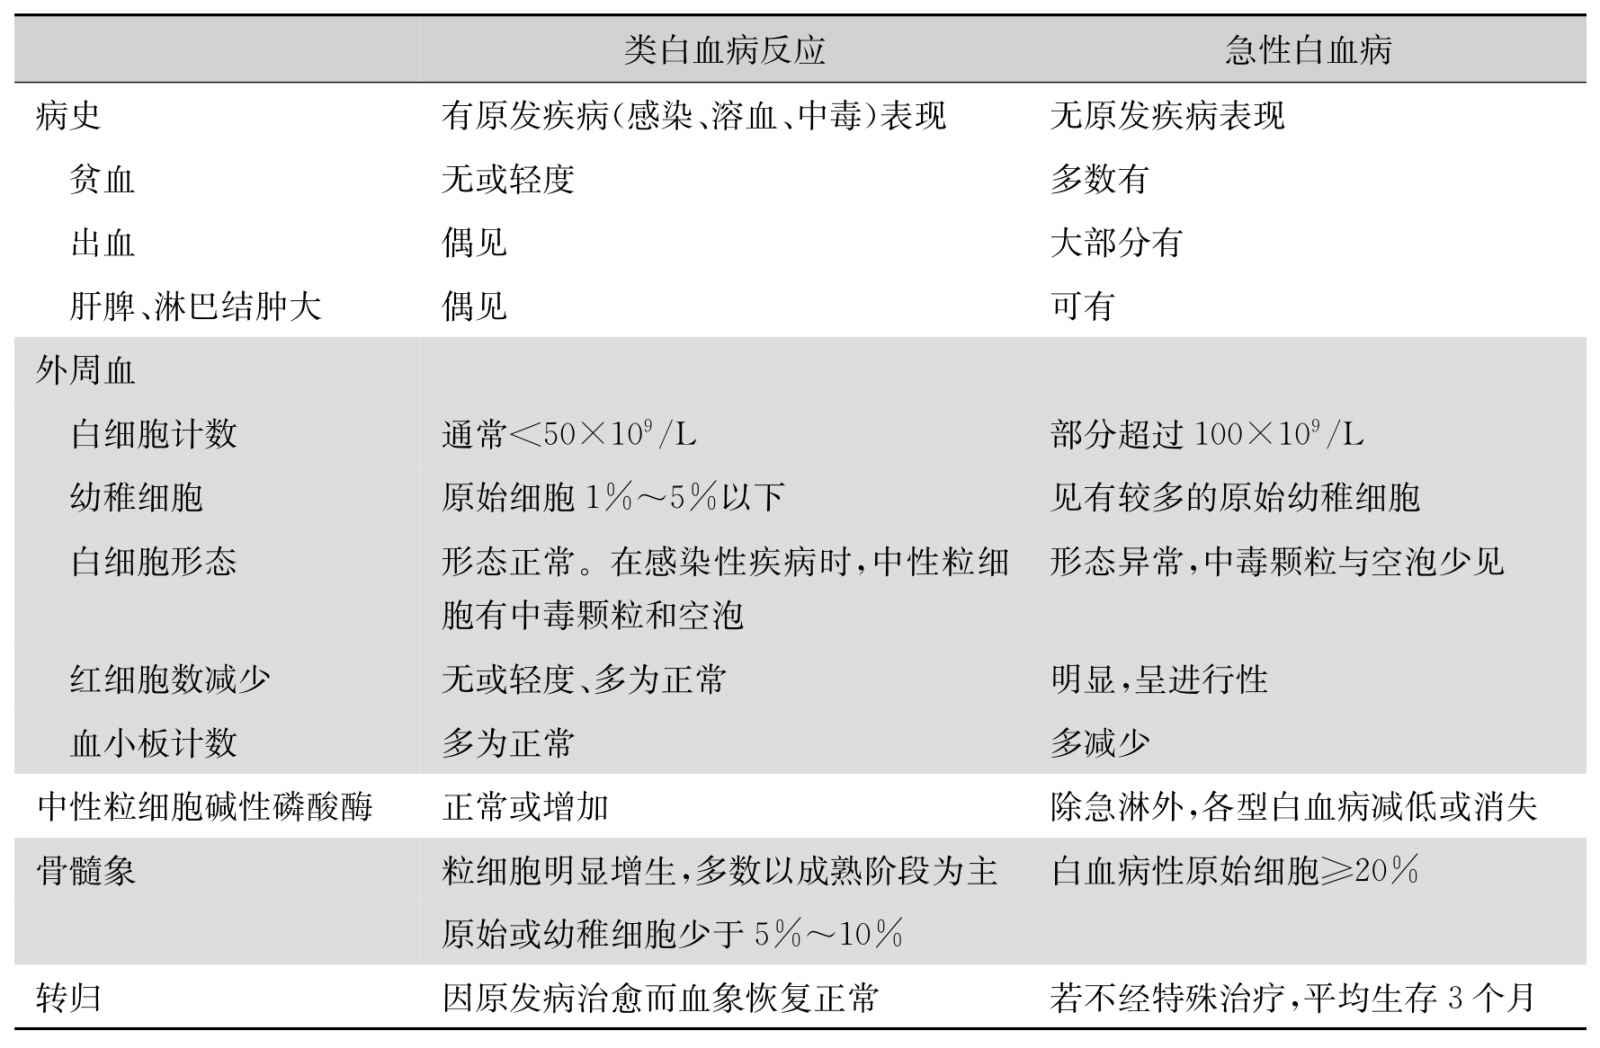
\includegraphics[width=5.91667in,height=3.875in]{./images/Image00026.jpg}
\end{table}

\subsubsection{五、组织细胞坏死性淋巴结炎}

组织细胞坏死性淋巴结炎,又称坏死性淋巴结炎、坏死增生性淋巴结病,是一种病因不明的非肿瘤性淋巴结肿大的疾病。

本病较少见,平均发病年龄30岁。起病急性或亚急性,特点如下:①95\%以上表现有发热:中、高度发热,热型呈不规则发热,也可呈弛张热,或反复间断发热,少数伴寒战,部分热程可长达2~3个月。②淋巴结肿大:多数有浅表淋巴结肿大以颈部最为常见,其次为腋窝及腹股沟,部分有压痛,也可有纵隔、腹膜后淋巴结肿大,少数有肝脾大。③少数有一过性皮疹、关节痛、多器官受累。④糖皮质激素治疗有效。

实验室检查:血象:白细胞计数常减少,可见核左移或异形淋巴细胞,轻度贫血,严重者血小板减少;对出现不明原因发热、浅表淋巴结肿大、白细胞减少,应想到本病的可能。淋巴结活检是本病诊断依据。病理学改变为淋巴结结构的部分或完全破坏,可见多少不等、大小不一的坏死灶,坏死灶周围组织细胞增多,坏死灶中可见浆细胞样单核细胞和免疫母细胞增生,无中性粒细胞浸润。由于本病的临床表现缺乏特异性,若未做淋巴结活检,误诊率高。本病需要与恶性淋巴瘤、结缔组织病、恶性组织细胞病、传染性单核细胞增多症相鉴别。

\subsubsection{六、Castleman病}

约近50\%的多中心型Castleman病表现为不明原因的长期发热,该病是一种少见的淋巴结增生性疾病,单中心型以纵隔、腹腔淋巴结肿大为多见;多中心型临床表现多样性、缺乏特异性,可以发热、浅表或深部淋巴结肿大,肝脾大,贫血,血小板减少,低白蛋白血症,免疫球蛋白升高(多克隆),易合并其他疾病或并发症如自身免疫疾病,POEMS,副肿瘤天疱疮,肾损害,淀粉样变。对疑诊本病,确诊需靠淋巴结活检病理检查,病理分为浆细胞型、透明血管型、混合型;临床分型包括单中心型、多中心型。

\subsubsection{七、朗格汉斯细胞组织细胞增生症}

一般多见于少儿,少见于成年人,临床表现:①发热:部分成年患者表现为长期发热、热型不规则,可呈周期性或持续性高热,使用抗生素无效,对激素敏感。②皮疹。③淋巴结肿大,肝、脾大。④肺部浸润:表现为轻重不等的呼吸道症状,但肺部体征不明显。肺部X线可见有弥漫性或网点状阴影。⑤骨骼破坏:长骨和扁平骨可发生溶骨性骨质破坏。⑥中枢神经系统:最常见的受累部位是丘脑-神经垂体区,弥漫性也可出现脑实质病变。有丘脑和垂体肉芽肿引起的尿崩症占该病的20\%~25\%。⑦其他:齿龈肿胀,牙齿松动,或突眼,或耳流脓或多饮多尿。病理检查是本病诊断依据,可行皮肤、淋巴结活检或病灶局部穿刺物病理检查。病理学特点是可见到特征性的分化较好的朗格汉斯组织细胞。该细胞CD1α、ATP酶、S-100蛋白、D-甘露糖苷酶均阳性。电镜下胞浆含有Birbeck颗粒。长期发热、尿崩症,要注意垂体朗格汉斯细胞组织细胞增生症。

\protect\hypertarget{text00035.html}{}{}

\subsection{5.3 风湿性疾病}

\subsubsection{一、成人斯蒂尔病}

成人斯蒂尔病(adult Still's
disease)是结缔组织病中引起长期不明原因发热的主要病因,占首位约50\%。成人Still病曾称为变异性亚败血症,是一种临床综合征。病因与发病机制尚未明确,可能与感染及自身免疫反应有关。发病年龄多于16~35岁,女性多见。表\ref{tab2-21}所示为文献报道的成人斯蒂尔病的主要临床表现。

\begin{table}[htbp]
\centering
\caption{成人斯蒂尔病的临床表现}
\label{tab2-21}
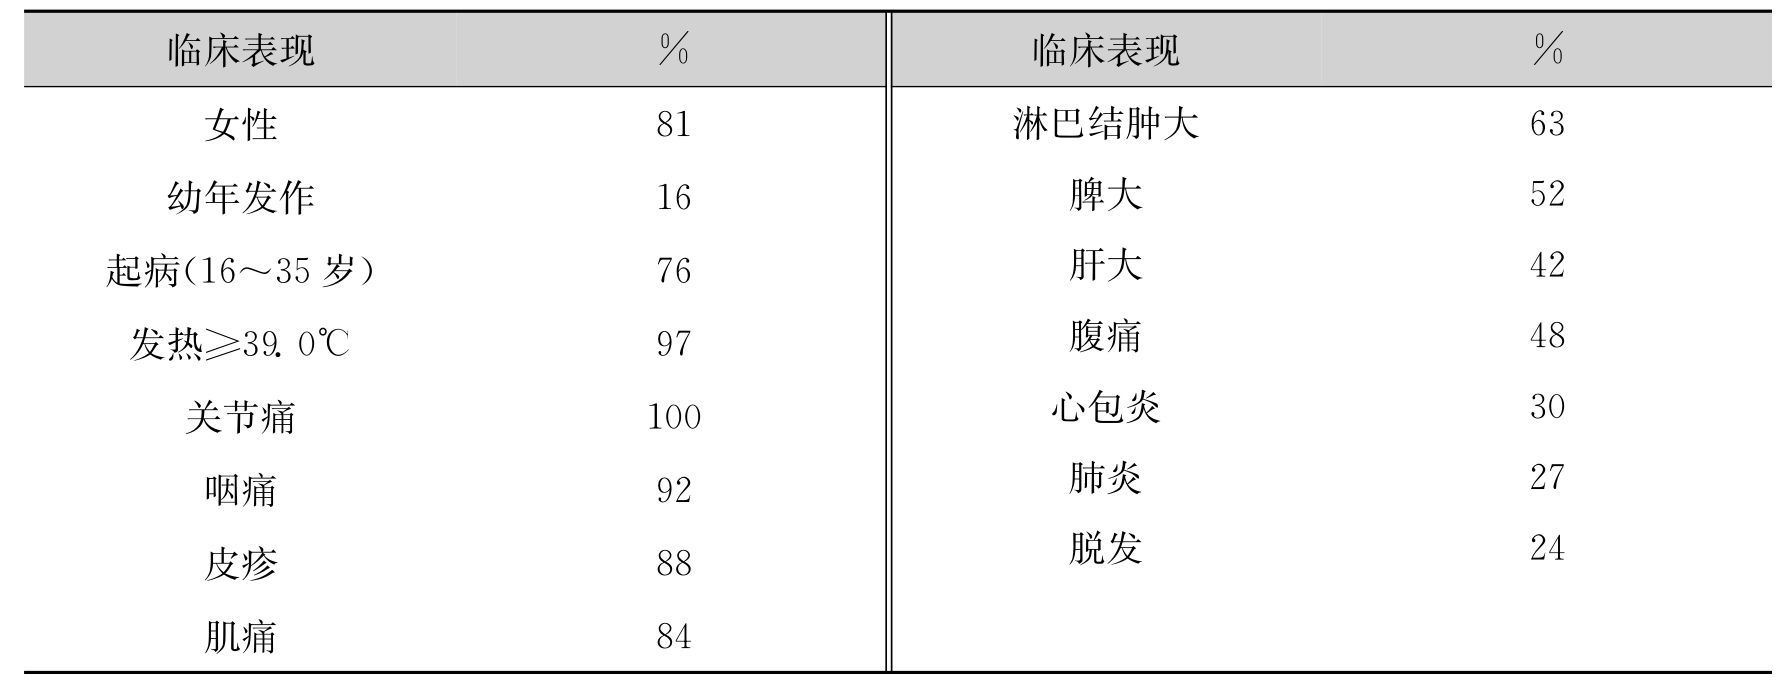
\includegraphics[width=5.9375in,height=2.29167in]{./images/Image00027.jpg}
\end{table}

\paragraph{1.临床特点}

\subparagraph{(1)发热:}

是本病的突出症状,多高于39℃,多数弛张热,也有不规则热,稽留热。热程1个月至1年,有报道平均5.3个月,常伴畏寒,但罕见有寒战,热程虽长,病情一般尚好,中毒症状不明显。各种抗生素治疗无效,而用糖皮质激素或非甾体类抗炎镇痛药能使体温降至正常。

\subparagraph{(2)皮疹:}

多为点状红疹,有时为斑丘疹或结节红斑,呈一过性,高热时出现,热退时消失。主要分布在躯干、四肢、手掌、足底。

\subparagraph{(3)关节痛或关节炎:}

可单关节或多关节受累。有时只有轻微关节痛。

\subparagraph{(4)其他:}

患者有咽痛,这是本病特征之一。部分有淋巴结肿大、肝脾大、胸膜炎、腹膜炎、心包炎、神经系统及呼吸系统损害等。除发热外有些患者起病时并非全部表现出上述症状,可能在病程中需要数月以至数年,才表现出来,亦可能始终未全部表现。

\paragraph{2.实验室检查}

(1)外周血白细胞总数增多,中性粒细胞核左移。

(2)血沉增快,C反应蛋白和免疫球蛋白升高。

(3)血清铁蛋白(SF)明显升高,铁蛋白>1000ng/ml(正常值上限的3倍)对诊断成人斯蒂尔病(AOSD)具有较高的阳性预测值(95.2\%),如果SF<1000ng/ml,则95.2\%认为不是AOSD;SF>1500ng/ml(正常值上限的5倍)阳性预测值为85.7\%,提示有临床表现者应高度怀疑AOSD。

(4)骨髓呈感染性骨髓象。

(5)2/3患者肝功能异常。

目前常用的诊断标准有日本成人Still病研究委员会制订的标准即Yamaguchi标准(1992):

主要指标:发热≥39℃,并持续1周以上;关节痛持续2周以上;典型皮疹;白细胞增高≥10×10\textsuperscript{9}
/L。

次要指标:咽喉痛;淋巴结肿大及(或)脾大;肝功能异常;类风湿因子和抗核抗体阴性。

符合5项条件含2项主要条件,排除感染性疾病及恶性肿瘤即可诊断。不典型的病例可无关节痛,一过性皮疹亦被疏漏。对于不典型病例必须充分排除其他引起长期发热的疾病才能诊断。

对诊为本病的患者必须长期随访,少数以后发展为淋巴瘤。

\subsubsection{二、系统性红斑狼疮}

长期的非感染性发热,兼有两个器官(如肾脏+浆膜;肾脏+关节;肝脏+心脏;关节+中枢神经系统)或多个器官受累的表现;发热伴血象白细胞减少、血小板减少、贫血或溶血性贫血者,应考虑系统性红斑狼疮(SLE)的可能。此病多见于女性,发病年龄多在21~40岁之间。以发热为主要临床表现者约占60\%~80\%。可以中、高热也可呈低热。首发症状的发热,伴皮疹与关节痛为多见。皮疹呈多形性,可从轻微的红斑乃至急性丹毒样病变或大疱,多见于面、颊、鼻、前胸、手、足等暴露处,但典型而有诊断价值的皮疹是蝶形红斑和盆状红斑。面部蝶形红斑虽为此病的特征性表现,但又非经常出现,国内报告阳性率为60\%~80\%。由于SLE症状复杂,如仅注意个别器官病变化,易误诊为风湿热、心包炎、胸膜炎、肾炎、类风湿关节炎、肝炎、特发性血小板减少性紫癜,甚至精神病等疾病。

美国风湿病学会1982年的SLE分类标准,对诊断SLE很有价值:①蝶形红斑:平的或高于皮肤的固定性红斑;②盘状红斑:面部的隆起红斑,上覆有鳞硝;③光过敏:日晒后皮肤过敏;④口腔溃疡;⑤关节炎:非侵蚀性关节炎;⑥浆膜炎:胸膜炎或心包炎;⑦肾病变:蛋白尿>0.5g/d或细胞管型;⑧神经系统病变:癫痫发作或精神症状;⑨血液系统异常:溶血性贫血或白细胞减少或淋巴细胞绝对值减少或血小板减少;⑩免疫学异常:狼疮细胞阳性或抗ds-DNA或抗Sm抗体阳性或梅毒血清试验假阳性
;\textcircled{11}
抗核抗体阳性。在上述11项中,如果有4项阳性,则可诊断为SLE,其特异性为98\%,敏感性为97\%。

SLE血清抗核抗体(ANA)是筛选结缔组织病的主要试验,阳性率达95\%~100\%,但特异性较差,其他结缔组织病、慢性活动性肝炎等均可呈阳性,诊断须结合临床与其他检查。血清抗双链去氧核糖核酸抗体(ds-DNA)特异性较高,且疾病早期即可出现,阳性率约62\%。抗Sm抗体是诊断SLE的标记抗体之一。特异性达99\%,但敏感性仅25\%。

系统性红斑狼疮样病象可由某些药物引起,称药物性狼疮综合征。可引起此综合征的药物可分为两类:①可引起红斑狼疮综合征的;②可使系统性红斑狼疮症状恶化的。属于第一类的药物有酰肼类药物(肼屈嗪、异烟肼等)、抗癫痫药物(如苯妥英钠)、普鲁卡因胺等。后者血清抗核抗体阳性率高达50\%~68\%,停药后症状在数周内消退,但血清抗核抗体阳性率可持续数月。此类药物性狼疮综合征罕有发生肾脏病变,且停药后不致再发。属于第二类的药物有青霉素、磺胺类、口服避孕药等,可使系统性红斑狼疮患者的症状恶化;但对正常人不致引起系统性红斑狼疮的病象或血清抗核抗体阳性。

\subsubsection{三、结节性多动脉炎(PAN)}

此病临床上少见,是一种累及中、小动脉的坏死性血管炎。此病的病理特点是多器官损害,主要累及心、肾、肺、肌肉、皮肤、关节等器官。患者以男性为多,年龄多在40~50岁之间,发热是最常见的症状,可高热也可低热。系统症状取决于受累器官。①皮肤表现:25\%~52\%患者有如血管性紫癜、结节红斑样皮肤结节、网状青斑、远段指(趾)缺血或坏死及雷诺现象;②关节肌肉表现:46\%~63\%患者可有关节炎、多发性肌痛和间歇性跛行;③神经系统表现:36\%~72\%患者有神经系统受累,以外周神经受累为主;④肾表现:45\%~83\%患者出现不同程度的肾损害,主要表现为蛋白尿,血、尿、细胞管型,高血压;⑤其他表现如胃肠道、心脏、肺、生殖系统等受累则有相应表现。

凡原因未明的长期发热,兼有多个互不相关的器官受累的表现,血象白细胞增多,须考虑此病的可能。实验室检查一般无特异性,可见轻度贫血、白细胞轻度升高,可见蛋白尿、血尿、管型尿,C反应蛋白增高,球蛋白升高,ANCA阴性,部分病例HBsAg阳性。诊断主要根据病理活检和血管造影。可行皮肤、肌肉、肾组织或睾丸活检。血管造影常见有肾、肝、肠系膜及其他内脏器官的中、小动脉有微小动脉瘤形成和节段性狭窄。1990年美国风湿病学会关于结节性多动脉炎的分类标准见表\ref{tab2-22},在10项中有3项阳性者排除其他结缔组织病并发的血管炎即可诊断。

此病在鉴别诊断上须多注意败血症、腹腔内恶性肿瘤、心肌炎、急性白血病、皮肌炎、系统性红斑狼疮、白塞病等疾病。

\subsubsection{四、肉芽肿性多血管炎(Wegener肉芽肿)}

Wegener肉芽肿是一种系统性、坏死性肉芽肿血管炎,主要累及上、下呼吸道及肾,同时也累及全身小动脉、静脉及毛细血管。本病临床上少见,无性别差异,以40~50岁为多见。

临床表现:①全身非特异症状如发热、关节痛、肌痛;②上呼吸道:表现为鼻、中耳、鼻窦的炎症;③肺部表现:肺病变见于70\%~80\%患者,可有咳嗽、咯血、胸痛和呼吸困难。X线示中下肺野结节和浸润或空洞;④肾病变:在病程中出现不同程度的肾小球性肾炎,重者可因进行性肾病变导致肾衰竭;⑤其他表现:部分有眼、皮肤、心脏受累的相应表现。

\begin{table}[htbp]
\centering
\caption{美国风湿病学会关于结节性多动脉炎的分类标准}
\label{tab2-22}
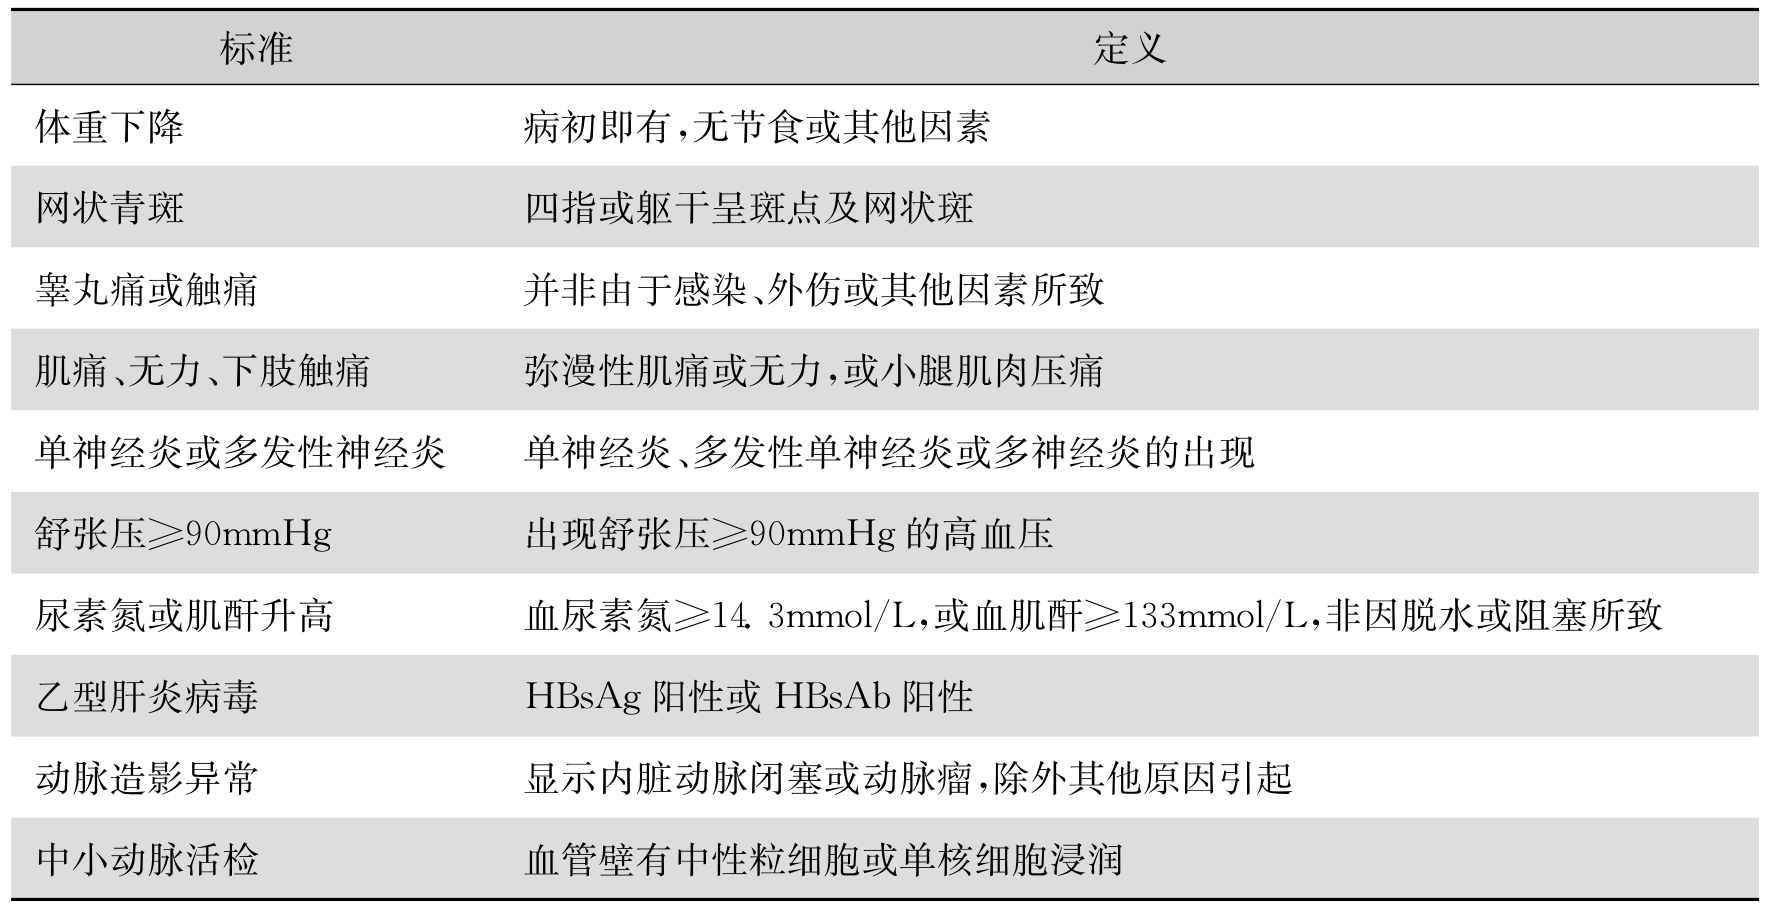
\includegraphics[width=5.91667in,height=3.03125in]{./images/Image00029.jpg}
\end{table}

实验室检查示:贫血、白细胞增多、血沉加快、类风湿因子低度阳性。血清中胞浆型抗中性粒细胞胞浆抗体(c-ANCA)阳性是诊断Wegener肉芽肿的重要参考指标。特异性为86\%,敏感性为78\%。

组织病理:鼻窦及鼻病变组织活检示坏死性肉芽肿及(或)血管炎。肾活检示局灶性节段坏死性肾小球肾炎。皮肤活检示白细胞破碎性血管炎。对临床表现有上、下呼吸道病变与肾小球肾炎者,实验室检查c-ANCA阳性,组织病理检查呈坏死性肉芽肿者可确诊。

此病与结节性多动脉炎的区别在于后者早期即出现肾脏损害,心脏通常明显受累。肺部症状主要为哮喘兼有嗜酸性粒细胞浸润和血中嗜酸性粒细胞增多等。此外还须与恶性中线性肉芽肿、特殊性传染性肉芽肿(结核性、梅毒性、真菌性等)、结节病、败血症、原发性肺癌等相鉴别。诊断主要依靠病理组织活检。

\subsubsection{五、混合性结缔组织病(MCTD)}

MCTD的特点为具有系统性红斑狼疮(SLE)、多发性肌炎、进行性系统性硬化、类风湿关节炎等多种结缔组织病的症状,肾脏损害轻。发热几乎经常出现。实验室检查显示高阳性率(达100\%)和高滴度的核糖核蛋白(RNP)抗体;荧光抗核抗体(FANA)达100\%阳性;而抗Sm抗体阴性,抗双链去氧核糖核酸抗体(ds-DNA)与狼疮细胞均呈低阳性率,C3、CH50均正常,提示MCTD是一种有特色的未分化结缔组织病。

\subsubsection{六、IgG4相关的硬化性疾病}

IgG4相关硬化性疾病是新近认识的一种疾病,是以累及胰腺以及胰腺外的肺间质,腮腺、泪腺、下颌腺等外分泌腺,胆道、后腹膜、肾脏、胃肠道、肝脏、乳腺等器官和脏器的慢性炎症性病变,血清学显示高γ球蛋白血症。病变部位以浆细胞浸润和纤维化为突出表现,可以检测到大量表达IgG4阳性的浆细胞,与自身免疫有关,且对类固醇激素治疗有效的一组异质性疾病。

患者可有不明原因发热、乏力、体重下降等全身表现,其他症状与受累器官组织有关,不同的器官组织受累有不同的表现,主要表现为局部压迫症状和相应腺体功能障碍。本病主要累及外分泌腺,多数患者胰腺受累,可表现为慢性轻中度腹痛、糖尿病。患者常因无痛性黄疸就诊,黄疸可呈波动性。涎腺、泪腺受累可出现腺体无痛性肿大,口眼干燥。此外,腹膜后纤维化的患者可出现腰背痛,因输尿管受压可能出现肾功能不全的表现。还有小管间质性肾炎、间质性肺炎、前列腺炎、乳腺炎等,症状均不特异。还可累及内分泌腺,包括垂体炎、Riedel甲状腺炎等。中枢神经系统受累很少见,但有硬脑膜、室管膜炎性假瘤和硬脑脊膜炎的报道。

多数患者出现高γ球蛋白血症,血清IgG、IgG4升高,IgG4/IgG比值升高,血清IgG4>1350mg/L对诊断AIP敏感性和特异性均很高,对诊断为AIP的患者,血清IgG>2200mg/L常提示胰腺外损害。

影像改变:累及胰腺时表现为胰腺弥漫性肿大,呈“腊肠样”,动态CT显示延迟强化。胰腺局灶性增大。内镜逆行胰胆管造影(ERCP)主胰管不规则狭窄,硬化性胆管炎患者胆管狭窄。肺部受累的CT表现主要分4型:实性结节型、圆形磨玻璃影型、肺泡间质型、支气管血管型。本病的肾损害主要在肾皮质,CT增强时表现为外围皮质圆形、楔形边界清楚的低密度影。

病理学组织淋巴浆细胞浸润、弥漫而致密的纤维化是这类疾病的特点;免疫组化显示,浸润的淋巴细胞主要是CD4\textsuperscript{+}
或CD8\textsuperscript{+} T细胞和IgG4\textsuperscript{+}
浆细胞,后者常超过30个/高倍镜。诊断依靠临床表现、血清学检查、影像学改变和病理学改变。

有报道一女性,56岁。不明原因发热3个月,腰痛1个月入院。胸部增强CT:后纵隔降主动脉周围软组织肿块,所示胸主动脉下段及腹主动脉旁不规则软组织影,包绕主动脉生长,下段腹主动脉旁及左侧髂总动脉旁不规则软组织影,包绕动脉生长,IgG
19.72g/L,IgG4:0.84g/L,行腹主动脉旁软组织活检术,病理:送检组织为大量增生纤维组织及脂肪和淋巴结一枚,淋巴结未见特殊病变,增生纤维组织中可见到大量浆细胞及中等量淋巴细胞,浆细胞浸润血管周隙及神经纤维束周围,酶标结果提示浸润淋巴细胞为CD4\textsuperscript{+}
T细胞,浆细胞分泌IgG为主,其中lgG4\textsuperscript{+}
细胞>20个/高倍视野,考虑IgG4相关硬化性疾病。

\protect\hypertarget{text00036.html}{}{}

\subsection{5.4 恶性肿瘤}

肿瘤性发热仅次于感染。恶性肿瘤患者长期发热见于两种情况:恶性肿瘤本身引起的发热和恶性肿瘤伴发感染所引起的发热。本处重点叙述肿瘤本身引起的发热。肿瘤热是由肿瘤细胞本身产生内源性致热因子,肿瘤迅速生长,瘤组织相对缺血、缺氧、坏死、出血引起吸收热;瘤组织坏死释放肿瘤坏死因子(TNF),TNF能诱导IL-1、IL-6的产生。TNF、IL-1、IL-6均为内源性致热原,而引起发热。

引起长期不明原因发热常见恶性实体瘤有原发性或继发性肝癌、肺癌、肾癌、甲状腺转移癌。较少见引起发热的有:结肠、卵巢、前列腺、乳腺、直肠、胰腺(无转移)和大脑恶性肿瘤、胃印戒细胞癌、松果体瘤、黑色素瘤、转移癌等。罕见引起发热的有嗜铬细胞瘤。此外,心房黏液瘤和胃、肾血管平滑肌脂肪瘤、小肠平滑肌瘤等是引起发热的良性肿瘤。

临床上,大多数恶性肿瘤引起的长期发热不超过38.9℃,如果超过此水平,一般提示感染性因素所致。热型多为弛张型或不规则型,患者通常无寒战,萘普生(naproxen)对肿瘤热有选择性解热作用。提示恶性肿瘤的其他症状是进行性消瘦、贫血等。对原因未明的低血糖状态、类白血病反应、游走性血栓性静脉炎、皮肌炎、纤维蛋白原缺乏症、红细胞增多症等情况,也须警惕恶性肿瘤的可能性;肾癌、肝癌、转移性肺癌、前列腺癌等,均可伴有红细胞增多症。癌也较常伴发于肺性肥大性骨关节病、皮肌炎、黑棘皮病等疾病。

肝癌:一些不典型或特殊表现的肝癌易被临床所忽视。肝大不明显,质不硬,甲胎蛋白反相间接血凝法或火箭电泳阴性,B超和CT有可能帮助发现本病,肝穿可找到确诊依据。

肾细胞癌很隐匿,约10\%的肾癌患者以发热为主要表现,通常仅表现为发热,无其他表现,有时伴乏力和消瘦,镜下血尿或血红细胞增多、血清碱性磷酸酶增高,可提示本病。B超、CT、选择性肾动脉造影有助于诊断。

嗜铬细胞瘤FUO,常见于发作性高血压病例,血压升高时体温增高,血压正常时体温降至正常。

肺癌通常不引起FUO,但部分病例在没有肺炎和肺不张的条件下表现为FUO。

心房黏液瘤可表现为发热、心脏杂音可呈现间隙性、体位性或缺如。血沉增快和贫血常见,超声心动图可确诊。

骨肉瘤也较常有发热的倾向。

\protect\hypertarget{text00037.html}{}{}

\subsection{5.5 中枢性发热}

下丘脑(间脑)综合征可由于炎症、肿瘤、外伤等引起,可导致长期不规则间歇发热,各项检查无急性感染的证据,血、尿培养均阴性,毒血症症状也不明显,应用各种抗生素而发热不能缓解。患者常伴有思睡、厌食或多食、肥胖、尿崩症、性功能减退以及自主神经功能紊乱症状等。

\protect\hypertarget{text00038.html}{}{}

\section{6 慢性低热}

体温上升达37.4~38℃(舌下测温)并除外生理性原因者称为低热;低热持续1个月以上者称为慢性低热。

有些高温作业的人、孕妇或女性排卵期,体温可较正常略高,但如离开高温环境或分娩后或排卵后,体温恢复正常,这种情况可称为生理性高体温,而非低热状态。

慢性低热可见于许多情况,一般可区分为器质性与功能性两大类(表\ref{tab2-23}),其中以器质性为常见;病因又以感染为多(表\ref{tab2-24})。

慢性低热的检查须注意下列情况:

\subsection{1.病史}

结核病史或结核患者接触史、咯血史、肝病史或黄疸史、局灶感染史、高温作业史等。

\subsection{2.体格检查}

需做全面体格检查,特别注意中耳炎、乳突炎、鼻窦炎、扁桃体炎、龋齿及齿根尖脓肿、前列腺炎等局灶性感染,贫血外貌,淋巴结与肝脾大,腹部压痛与包块,肾区叩击痛与压痛,脊柱压痛与纵轴叩击痛等。女性患者须考虑妇科检查。

\subsection{3.化验检查}

应作血、尿、便三项常规检查和血沉测定。未能除外感染或结缔组织病时,做抗链球菌溶血素“O”滴度测定、血清蛋白电泳测定、血中狼疮细胞检查,以及有关的血清免疫学检查。怀疑肝脏疾病时做常规肝功能试验。结核菌素试验强阳性有助于活动性结核病的诊断,但阴性未能排除此病。患者有未能解释的贫血时,须做骨髓象检查。

\begin{table}[htbp]
\centering
\caption{慢性低热疾病分类}
\label{tab2-23}
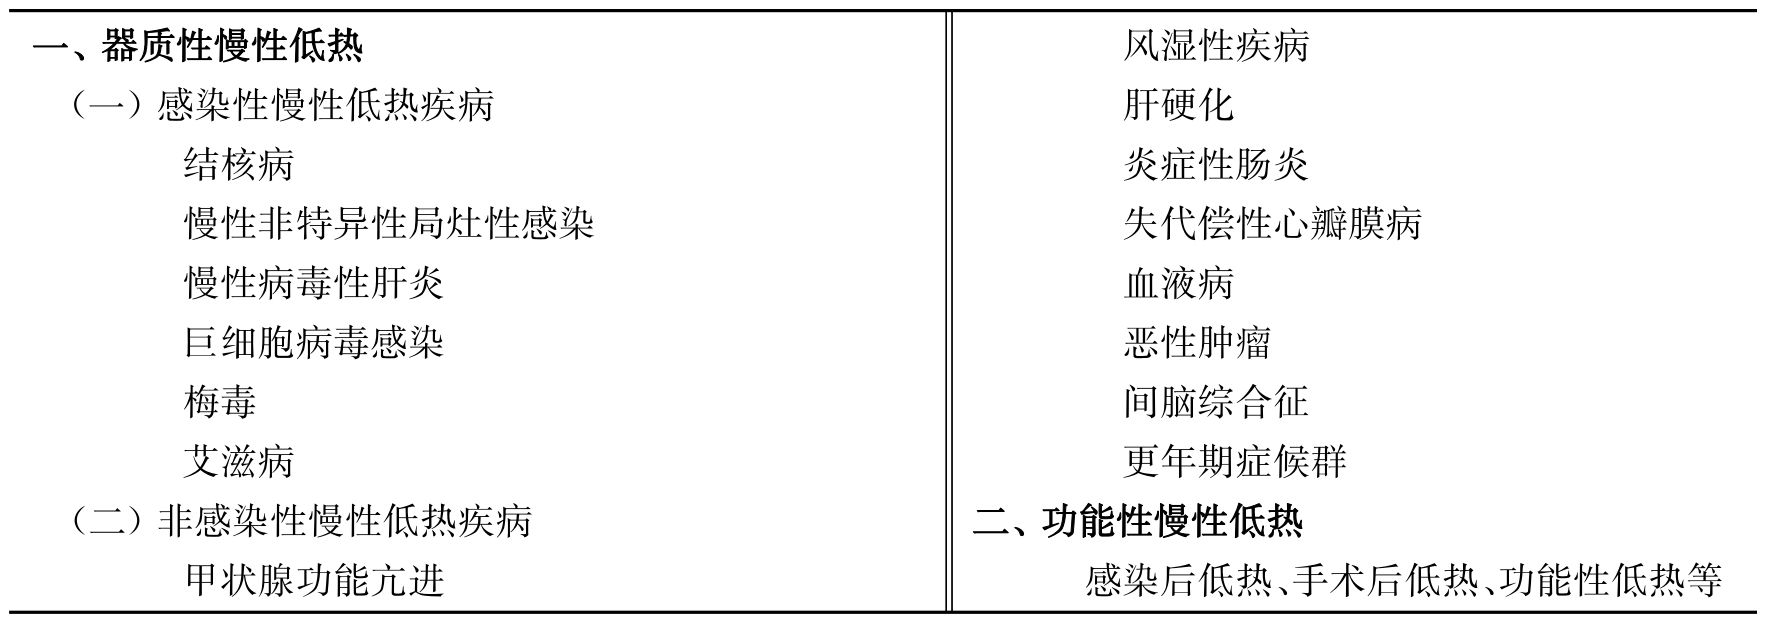
\includegraphics[width=5.875in,height=2.08333in]{./images/Image00030.jpg}
\end{table}

\begin{table}[htbp]
\centering
\caption{800例低热的原因分析}
\label{tab2-24}
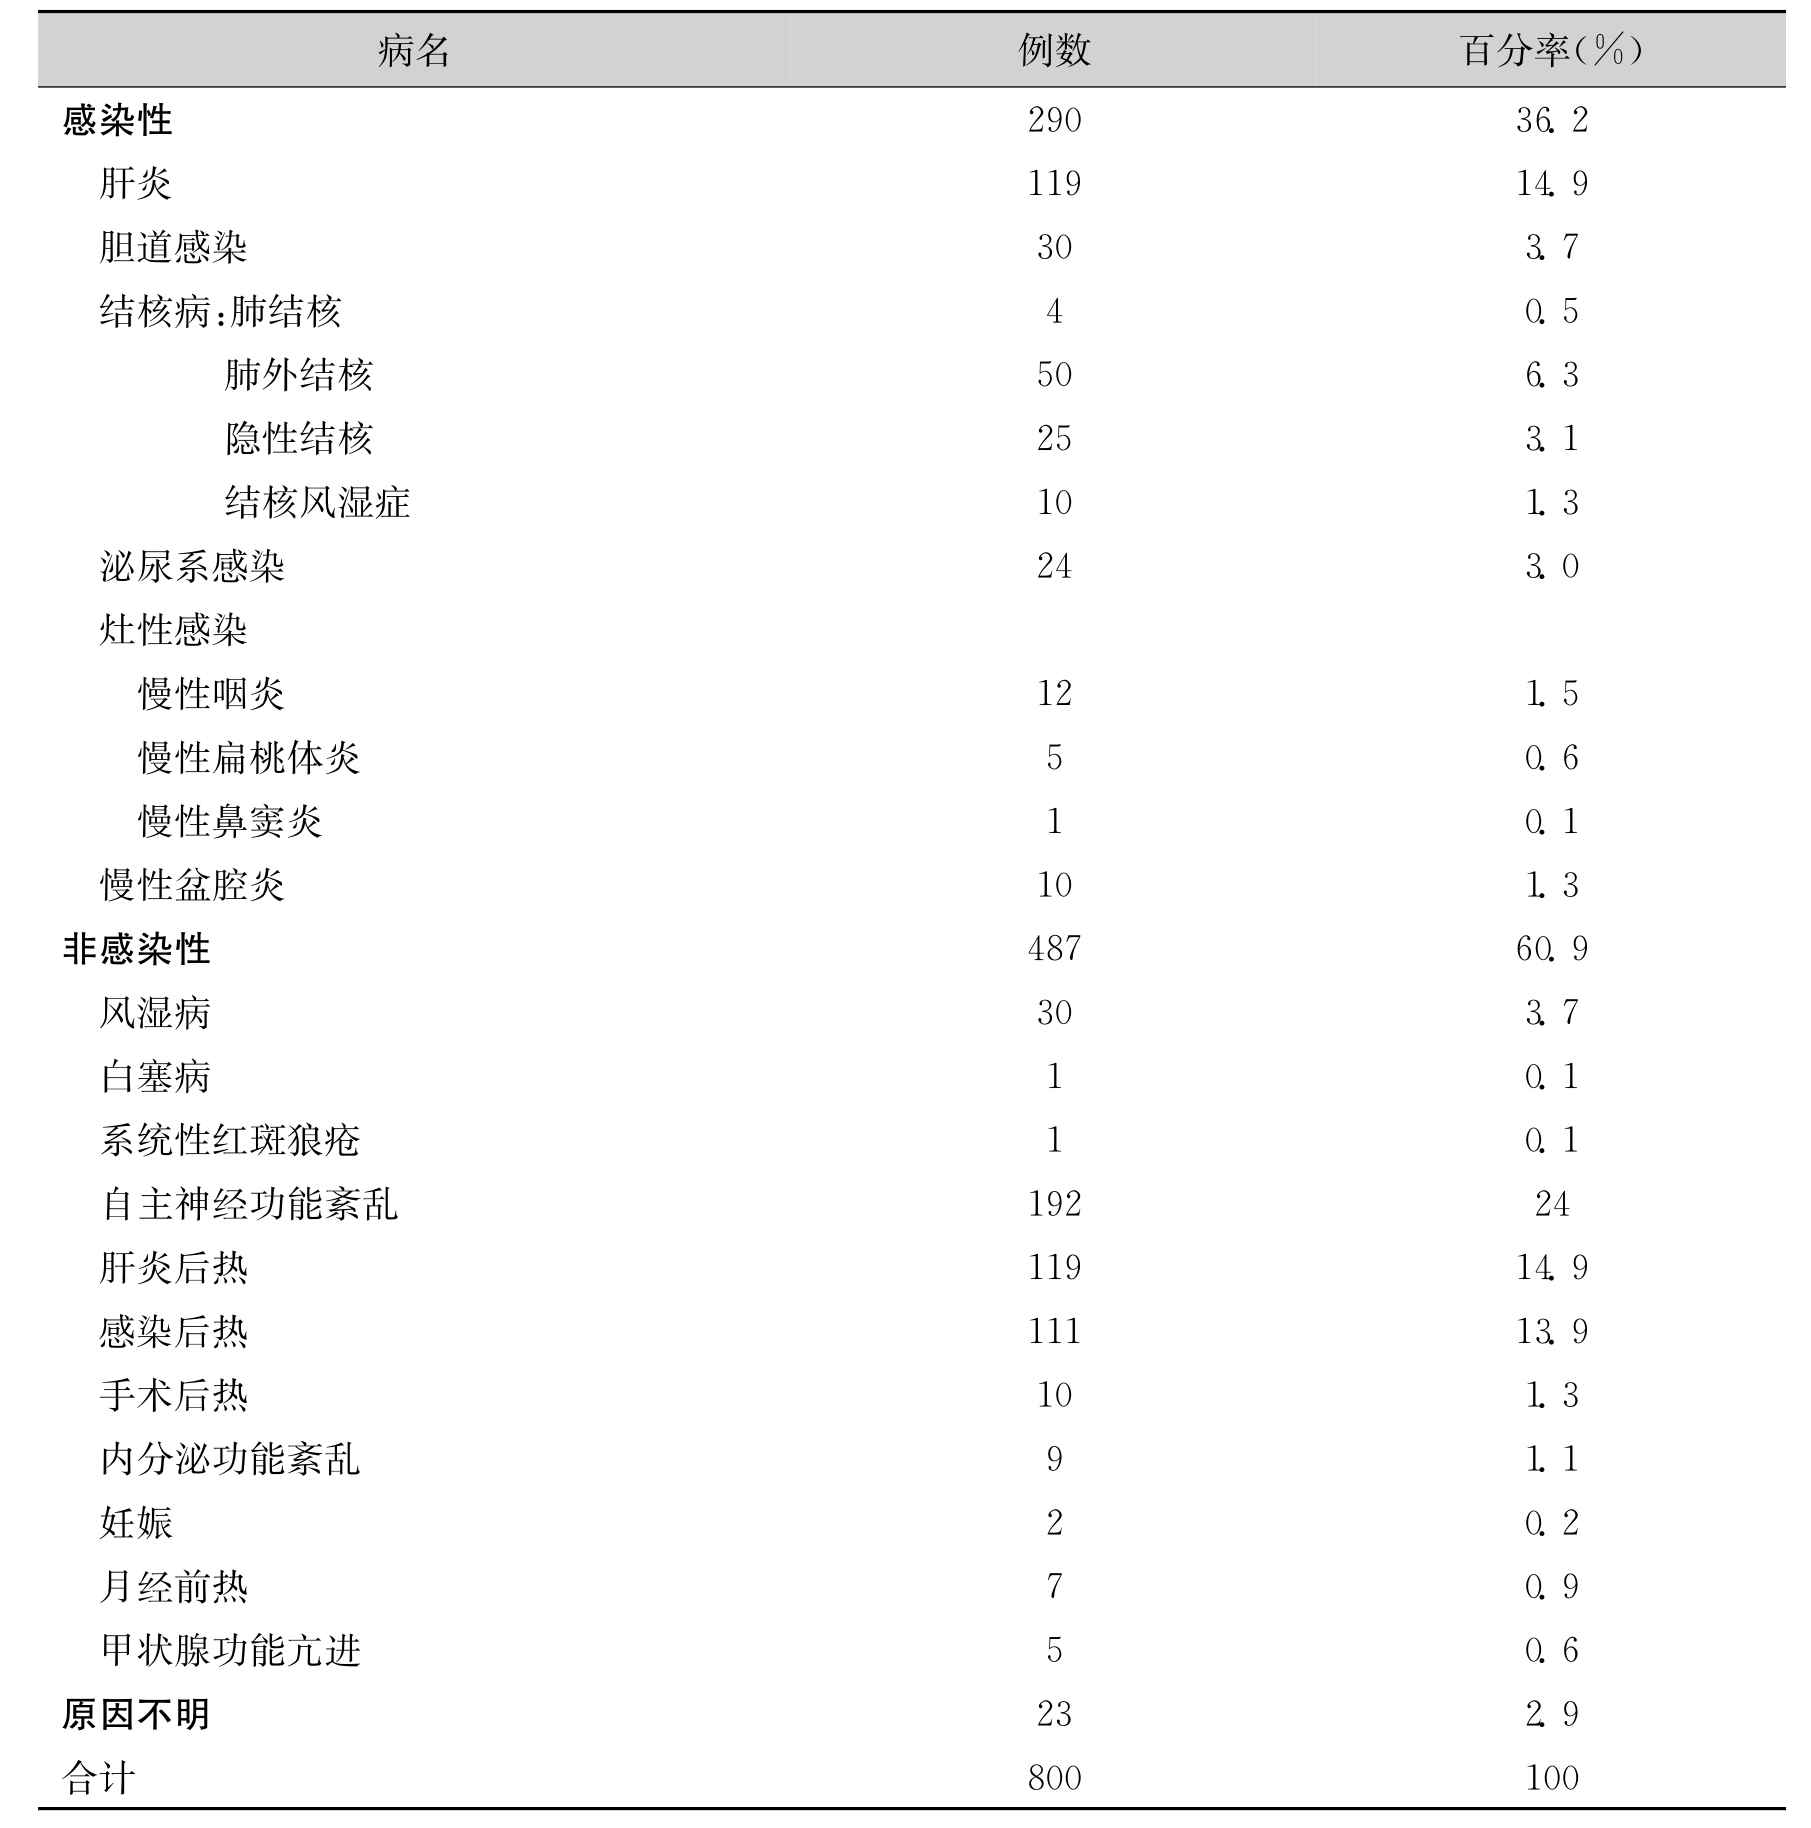
\includegraphics[width=6.03125in,height=6.08333in]{./images/Image00031.jpg}
\end{table}

\subsection{4.器械检查}

X线胸部透视应作为常规检查,需要时摄片。心电图描记、甲状腺吸131碘试验、超声肝区检查、胃肠钡餐透视与钡剂灌肠、眼底检查等,可按需要选择行之。未除外胆道感染者,有指征作十二指肠引流及(或)胆囊造影检查。疑为胸腹占位性变时做B超与CT检查。

\protect\hypertarget{text00039.html}{}{}

\subsection{6.1 器质性慢性低热}

\subsubsection{6.1.1 感染性慢性低热疾病}

\paragraph{一、结核病}

患者有慢性低热与结核中毒症状时,首先应考虑结核病。最常见的是肺结核,但早期可无呼吸系统症状与体征,X线透视检查也不一定完全可靠。有怀疑时应做胸部照片检查。

诊断困难者为肺外结核。肺外结核种类繁多,包括多系统、多脏器、多部位、多种类型的结核性病变。诊断比肺结核明显困难。为了避免误诊或漏诊,须注意:①进行全面、细致地病史询问和体检;②深部结核病灶或隐性病灶须选择X线、B超、CT、纤维内镜,甚至开腹探查协助诊断,从病理活检中确定诊断;③结核菌素试验;④如未排除隐性病灶的存在应采取积极的有效抗结核诊断性治疗,疗程不少于4~6周。由于近年来结核病有复燃之势,诊断性治疗临床症状奏效之后,对疑似病例仍需继续正规治疗,不能半途而废。

诊断上较难的肺外结核病变,如肾结核大多数发生于20~40岁之间,主要症状不表现于肾而表现于膀胱,约75\%~85\%患者有膀胱刺激征,如尿频、尿急与尿痛。主要化验所见为血尿,多为镜下血尿,有时为肉眼血尿,常间歇出现。其他症状为低热、腰痛、纳差、盗汗、消瘦、倦怠等。

肝结核少见,也可引起慢性低热,结核菌素试验阴性不能除外此病,临床上不易诊断。CT扫描有助于发现粟粒病灶。

骨结核主要侵犯儿童与年轻成人。骨结核好发于脊椎,最常侵犯腰椎或胸椎,易于漏诊,腰背部局限性隐痛及(或)固定性局限性脊椎压痛提示此病的诊断。

肠系膜淋巴结结核,主要侵犯儿童与青少年,常与肠结核及结核性腹膜炎并发。凡年轻患者有原因未明的慢性发热与结核中毒症状、血沉加快、营养不良及与饮食无关的腹痛,即使腹部未触及包块,也须考虑腹腔内淋巴结结核的可能性,结核菌素试验强阳性(但阴性未能除外本病)和腹部X线摄片发现钙化灶,有力地支持本病。抗结核药物诊断性治疗奏效时可证实临床诊断。本病往往须手术探查方能明确诊断。

女性生殖器结核,主要侵犯附属器官,症状不典型,临床诊断不易。发病多在20~40岁之间,往往有低热、倦怠、下腹痛、盗汗、体重减轻等症状。妇科病征则有月经稀少,闭经与不育。遇见女性结核患者,尤其是肺结核病或腹膜结核,或患者有全身性结核病症状而找不到病灶,而同时有不育症,月经稀少或闭经,应考虑女性生殖器结核的可能性。

肾上腺结核少见,此病临床上往往表现为Addison病。国内一组3例原发病为肺结核,肾上腺结核均经CT证实。

\paragraph{二、慢性非特异性局灶性感染}

扁桃体、齿根、鼻窦、中耳、乳突、胆道、肠道、肾盂、前列腺、女性内生殖器等处的慢性炎症,也有引起慢性低热的可能,但以不规则的波动性发热为多见。患者除局部病征之外,并常有精神体力欠佳、血沉轻度加快等表现。有的患者伴有心悸、多汗、皮肤划痕症等自主神经功能紊乱症状。局灶性感染根治后,低热及其他症状也随之消退。

链球菌感染后状态:临床上可见到一些扁桃体炎或咽炎之后出现低热、关节酸痛。心率加快、抗“O”增高,血沉正常或轻度加快,咽拭子培养可证明乙型溶血性链球菌,心电图检查可发现短暂的期前收缩或(及)轻度S-T段与T波改变。无心脏增大与心杂音。给予青霉素或其他抗菌药物治疗,常于短期内解热。关节痛及其他症状均消失;如病情改善不明显,加用小剂量泼尼松也奏效。这种情况可称为链球菌感染后状态,如经上述治疗病情仍无好转或有再发,须考虑为风湿热或其他并存的疾病。

\paragraph{三、慢性病毒性肝炎}

慢性无黄疸型病毒性肝炎可引起低热。患者除有食欲减退、肝区隐痛、肝大压痛等肝炎表现外,常兼有多汗、易兴奋、失眠等自主神经功能紊乱症状。低热于休息时较低,活动或劳累略有升高,热程可累月甚至经年。患者肝功能多有异常,还可在血清中检出特异性肝炎标志物。十二指肠引流有时可发现“B”、“C”管的胆汁中白细胞数增加,容易与胆道感染相混淆。胆汁培养无细菌生长,镜检无寄生虫发现,诊断性治疗不奏效,据此可与慢性胆道感染相区别。

\paragraph{四、巨细胞病毒感染}

近年有人注意到巨细胞病毒感染所致的持续微热状态。这种病毒感染又称为全身性巨细胞性包涵体病,其临床表现变异很大。可表现为类似传染性单核细胞增多症的综合征,但嗜异性凝集反应阴性。也可引起慢性肝脏病变。表现为慢性无黄疸型肝炎。诊断须依靠血、尿的病毒分离培养,巨细胞病毒补体结合试验,尿路上皮细胞中发现细胞核内包涵体等。

\paragraph{五、梅 毒}

梅毒第二期以后的表现较为复杂。如患者有梅毒接触史,血清梅毒抗体特异性试验阳性,而有原因未明的慢性低热,应考虑此病的可能性。

\paragraph{六、艾滋病}

艾滋病亦可表现为慢性低热。

\paragraph{七、其 他}

也见有个案报道布鲁杆菌病、伤寒、POEMS、恶性间叶瘤也可引起低热。

\protect\hypertarget{text00040.html}{}{}

\subsubsection{6.1.2 非感染性慢性低热疾病}

\paragraph{一、甲状腺疾病}

甲状腺功能亢进、甲亢危象,亚急性甲状腺炎、甲状腺癌中滤泡细胞型者、少数桥本病表现为亚急性甲状腺炎或甲亢,均可有不同程度发热和出汗,这些患者发热同时多有高代谢症候群。

\paragraph{二、风湿性疾病}

风湿性疾病以发热为主要临床表现,因此呈慢性低热者亦有之。这种情况可见于风湿热、系统性红斑狼疮、结节性多动脉炎、皮肌炎,结节病、大动脉炎、小血管炎也见有个案报道表现为低热。

\paragraph{三、肝硬化}

肝硬化患者约1/4~1/3有发热,大多由于肝细胞坏死或肝内炎症等活动性病变所致。部分病例呈低热,常未能发现任何发热的原因。发热较高时往往提示合并感染。

\paragraph{四、炎症性肠病}

Crohn病及溃疡性结肠炎,均可有慢性低热,提示轻度的炎症活动。

\paragraph{五、失代偿性心瓣膜病}

失代偿性心瓣膜病可能有持续的低热,由于淤血性支气管炎、细小的肺梗塞或血栓性静脉炎等所致。或认为在充血性心力衰竭时,由于心排血量降低、皮肤血流量减少以及水肿的隔热作用,使散热减少,再由于呼吸困难时呼吸肌运动量增加,使热的产生有所增加,故可有低热。

如患者持续低热兼有关节(肿)痛,心律失常如心房颤动、阵发性心动过速、期前收缩的出现,洋地黄耐受量降低,新的瓣膜病变杂音的出现或心杂音的改变(包括强度增加与音质改变)等情况,则应考虑活动性风湿性心脏病。如持续低热兼有栓塞现象(皮肤或结膜瘀点),则提示并发亚急性细菌性心内膜炎的可能性。

\paragraph{六、血液病}

重症贫血患者常有低热,乃由于基础代谢率稍有增高之故。慢性白血病与恶性淋巴瘤也可有低热。少见病Castleman病也可以长期低热。

有报道:男,34岁,反复午后低热11年,37.2~37.5℃,浅表淋巴结肿大,最大直径2cm,病初淋巴结活检示淋巴结反应性增生,短期糖皮质激素治疗淋巴结有缩小,但仍反复低热,11年后除了浅表淋巴结肿大外、肝脾大,白细胞低、小细胞低色素性贫血;高球蛋白血症,多克隆性免疫球蛋白及轻链升高;PT、APTT延长,反应性浆细胞增多。低氧血症,双肺弥漫性病变,蛋白尿,镜下血尿,B超示双肾弥慢性病,淋巴结活检示Castleman病。

\paragraph{七、恶性肿瘤}

恶性肿瘤有发热的倾向,特别是肺癌、肝癌、结肠直肠癌。低热一般见于无并发症和无进行性急剧坏死的恶性肿瘤。中年以上患者有慢性低热与血沉加快,虽无任何其他病征,也须注意深部恶性肿瘤的可能性。

\paragraph{八、间脑(下丘脑)综合征}

间脑由丘脑、丘脑底、下丘脑和第三脑室周围结构所组成,是大脑皮质和各低级部位相互联系的重要机构。间脑综合征较下丘脑综合征有更广的范围,二者都可引起体温调节障碍,以及一系列自主神经失调症状,症状还有发作性的特点。

下视丘视前区两侧急性病变常引起体温迅速升高;慢性起病的间脑综合征则不少有低热。发病以21~40岁为多。据我院1963年总结30例的经验,病因以感染为多,其次为脑外伤、肿瘤、中毒等,但也有原因未明者。

间脑功能十分复杂,间脑病损主要有下列表现:

\subparagraph{1.自主神经功能紊乱症状}

如多汗或无汗;多尿或少尿,脉快或脉慢,血压升高或降低,发作性头昏,皮肤划痕症等。此外尚可表现为半侧感觉障碍、半侧水肿。半侧皮肤发红、半侧无汗或多汗等。

\subparagraph{2.内分泌代谢障碍}

如肥胖,糖耐量曲线异常,剧烈饥饿感、皮肤不对称性水肿,性欲减退,月经不正常,不育等。

\subparagraph{3.睡眠障碍}

如嗜睡或失眠,倒错性睡眠(白天嗜睡,夜间不睡)。

\subparagraph{4.体温调节障碍}

以慢性低热最为多见。低热的特点是:①对解热药呈异常反应;非间脑病变时,服阿司匹林后开始时皮肤温度升高,而在间脑病变时呈倒错反应(即开始时皮温下降)或无反应。②两半侧身体皮肤温度不对称现象,在间脑病变时相差甚明显,如相差在0.4~
0.5℃时可认为是病理性。③24小时体温曲线正常人在下午较高,连续测量数天在间脑病变有时上午较高。

间脑综合征的诊断主要根据:①有关的既往病史;②在短期内出现上述大部分症状;③症状分布为全身性或半侧性;④有发作性的特点;⑤脑电图各导联阵发性出现θ波有助于诊断。其病因的诊断较难,必须联系下丘脑的生理功能,结合有关下丘脑靶腺反馈机制,头颅CT和磁共振等影像学特征作出诊断。

\paragraph{九、更年期症候群}

更年期症状与体征均与雌激素水平下降有关,常见症状为阵发性潮红,尤其面颈部皮肤多见,可持续数年,其次为发热和出汗,也多有阵发性规律,感觉异常,手脚发凉,头晕头痛、失眠,健忘,精力不集中,精神紧张,焦虑,神经质等更为多见,血浆雌二醇及孕酮降低,促卵刺激素升高,促黄体生成素多正常,结合年龄和闭经史诊断较易。

\protect\hypertarget{text00041.html}{}{}

\subsection{6.2 功能性低热}

功能性低热的临床特征是患者体温较正常人升高约0.3~0.5℃左右,一般不超过38℃。经反复体检,病理学和实验室检查,除体温升高外未见其他异常,长期观察,一般情况良好,不影响正常工作和生活,经抗感染、抗结核、抗风湿等治疗无效。

\subsubsection{一、感染后低热}

在其前往往有细菌、病毒、衣原体、原虫等感染,特别多见于病毒感染后。此时体温调节中枢对体温的调节功能仍未恢复正常所致。

\subsubsection{二、手术后低热}

手术后可以有术后吸收热,一般在术后6~8小时开始发热,持续3~5天可自行缓解,但部分患者低热持续,而与手术相关的切口等均正常。

\subsubsection{三、功能性低热}

多见于青年女性,为一种原发性低热,日间温差不大(相差0.5℃左右),体温昼夜规律失常。晨间午前往往较下午晚间略高,体力活动体温可不升或有时反而下降。持续数月、数年,体温往往在偶然或患者不注意情况下自动下降。患者又常兼有多汗、手颤、皮肤划痕症、呼吸性不整脉、怕冷、心悸、失眠等自主神经功能紊乱的表现。

\subsubsection{四、夏季低热}

低热仅发生于夏季,秋凉后自行退热,每年如此反复出现,连续数年后多可自愈。多见于幼儿,因体温调节功能不完善,夏季身体虚弱,且多发生于营养不良或脑发育不全者。

\subsubsection{五、其 他}

妊娠初期也可有低热现象。部分妇女月经前7~10天体温上升至37.5℃,月经来潮后体温降至正常。

功能性低热的诊断需根据较长时间的观察,排除各种器质性疾病,如肺外结核、甲亢、恶性肿瘤,在女性尤需注意卵巢癌,男性患者诊断功能性低热需慎重。

\protect\hypertarget{text00042.html}{}{}

\section{参考文献}

1.胥婕,等.北京地区250例严重急性呼吸综合征患者临床分析.中华结核和呼吸杂志,2003,26(11):683-685

2.倪安平.衣原体的肺部感染.中华结核和呼吸杂志,1998,21(9):516-517

3.李丽,等.鹦鹉热衣原体肺炎一例.中华结核和呼吸杂志,1999,22(11):662

4.刘忠达,等.恙虫病肺部合并症50例临床分析.中华结核和呼吸杂志,2002,25(8):478-480.

5.陈晓红.恙虫病致肺损害46例.中华传染病杂志,2002,20(5):312-313

6.张溪林,等.恙虫病致急性肺损伤/急性呼吸窘迫综合征.中华传染病杂志,2003,21(6):436-437

7.黄学焕,等.96例肺下叶结核的诊断与鉴别诊断.中华内科杂志,1994,33(8):515

8.梁思礼,等.类鼻疽肺病四例报告与文献复习.中华结核和呼吸杂志,1994,17(3):168-170

9.陆慰萱,等.嗜肺军团杆菌肺炎37例综合分析.中华结核和呼吸杂志,1997,20(2):91-94

10.张斌,等.变态反应性支气管肺曲霉病.中华结核和呼吸杂志,1999,22(6):377-378

11.文仲光,等.肺毛霉病------附二例报告.中华内科杂志,1998,37(5):327-329

12.张可,等.艾滋病合并卡氏肺孢子虫肺炎的临床特点及诊断方法.中华结核和呼吸杂志,2002,25(8):475-477

13.金明根,等.生食鳖所致比翼线虫病的临床分析.中华结核和呼吸杂志,1998,21(10):611

14.燕航,等.肾移植术后巨细胞病毒肺炎的诊治.中华器官移植杂志,2001,22(5):298-300

15.徐志松,等.异基因骨髓移植后巨细胞病毒肺炎的临床研究.中华结核和呼吸杂志,2004,27(9):646-647

16.徐小元,等.人禽流感的流行病学与生物学.中华医学杂志,2004,84(5):353-354

17.林江涛.人禽流感的诊断治疗策略.中华医学杂志,2004,84(5):355-356

18.刘又宁,等.中国城市成人社区获得性肺炎665例病原学多中心调查.中华结核和呼吸杂志,2006,29:3-8

19.中华医学会呼吸病学分会感染学组.肺真菌病诊断和治疗专家共识.中华结核和呼吸杂志,2007,30:821-834

20.唐可京,等.肺接合菌的诊治.中华结核和呼吸杂志,2009,32:793-796

21.Gupta SK,et al.Evaluation of the Winthrop-University Hospital
criteria to identify Legionella pneumonia. Chest.2001,120(4):1064-71

22.Agarwal R,et al.Aspergillus hypersensitivity in patients with
chronic obstructive pulmonary disease:COPD as a risk factor for
ABPA?Med Mycol.2010,48:988-994

23.中华人民共和国国家卫生和计划生育委员会.人感染H7N9禽流感诊疗方案(2013年第2版).中华临床感染病杂志,2013,6(2):65-67

24.韩明锋,等.国内102例人感染H7N9禽流感特点初步分析.传染病信息,2013,26(2):68-70

25.权菊香,等.2013年我国H7N9型禽病毒流感分析.中国临床药理学杂志,2013,29(6):426-428

26.杨钧,等.甲型H1N1流感合并肺炎的影像表现.中华放射学杂志,2010,44(2):119-122

27.陈枫,等.重症及危重症甲型H1N1流感肺炎的影像表现.中华放射学杂志,2010,44(2):123-126

28.罗宏,等.新型甲型H1N1流感重症患者肺部影像学变化及临床特点.中华结核和呼吸杂志,2010,33(6):415-418

29.Fujitani S,et al.Pneumonia due to Pseudomonas
aeruginosa:partⅠ:epidemiology,clinical diagnosis,and
source.Chest,2011,139(4):909-919

30.廖纪萍,等.军团菌肺炎的临床诊治进展.国际呼吸杂志,2007,27(21):1632-1636

31.姚郁林,等.肺出血型钩端螺旋体病113例X线诊断体会.山东医药,2008,48(25):47

32.刘又宁,等.中国1998年至2007年临床确诊的肺真菌病患者的多中心回顾性调查.中华结核和呼吸杂志,2011,34(2):86-90

33.姚婉贞.侵袭性肺曲霉病的诊断与治疗.中华结核和呼吸杂志,2011,30(11):812-814

34.何礼贤,等.慢性阻塞性肺疾病合并侵袭性肺曲霉病的病理生理特点及其诊断策略.中国真菌学杂志,2011,6(5):257-260

35.何礼贤.肺孢子菌肺炎的诊断与治疗.中华结核和呼吸杂志,2007,30(11):802-805

36.张波.急性间质性肺炎的诊断与治疗.上海医学,2009,32(10):843-844

37.庄谊.隐源性和继发性机化性肺炎临床和影像学特点分析.实用临床医药杂志,2011,15(19):147-149

38.降钙素原急诊临床应用专家共识组.降钙素原急诊临床应用的专家共识.中华急诊医学杂志,2012,21
(9):944-951

39.蔡闯,等.2009年甲型H1N1流感研究近况.中国急救医学,2009,29(6):553-555

40.权菊香,等.2013年我国H7N9型禽病毒流感分析.中国临床药理学杂志,2013,29(6):426-428

41.谢正德.儿童EB病毒传染性单核细胞增多症临床特征及诊断标准.实用儿科临床杂志,2007,22(22):1759-1760

42.林特夫,等.细菌L型感染的意义和研究进展.蚌埠医学院学报,2006,31(2):111-115

43.童强,等.肾移植术后巨细胞病毒性肺炎的诊断与治疗.解放军医学杂志,2006,31(7):716-771

44.倪莲芳,等.组织细胞坏死性淋巴结炎68例临床分析.中华医学杂志,2010,90:3147-3149

45.谭明旗,等.组织细胞性坏死性淋巴结炎48例临床分析.中国实用内科杂志,2003,23(1):51

46.刘本似,等.我国西藏地区兔热病(土拉菌病)14例报告.流行病防治研究,1974,(3):224

47.何远学.钩端螺旋体病26例临床分析.中国热带医学,2006,6(10):1830

48.林瑞炮,等.凶险型恶性疟疾临床分型及治疗.中华传染病杂志,2002,20(5):317

49.郑德福,等.1964-2011年中国大陆人体旋毛虫病流行分析.寄生虫病与感染性疾病,2011,9(3):119

50.李兴福,等.急性风湿热诊断的相关问题.临床内科杂志,2005,22(10):652

51.赵丹,等.登革热预警技术研究进展.中华流行病学杂志,2012,33(5):540

52.张顺先,等.我国2005~2012年登革热流行特征分析.中国医药指南,2013,11(16):401

53.罗雷,等.广州市1978至2006年登革热流行病学特征分析.中华传染病杂志,2008,26(8):490

54.查震球,等.175例恙虫病病例的临床和流行病学特征研究.中华疾病控制杂志,2010,14(8):720

55.张萌,等.中国恙虫病流行态势及预防控制.中华流行病学杂志,2011,32(4):419

56.杨晴,等.恙虫病临床特点分析.中华实验和临床感染病杂志(电子版),2011,5(1):42

57.胡相,等.一起人的类丹毒流行病学调查.中华预防医学杂志,1980,14(4):213

58.黄奕江.类鼻疽病的诊断与治疗.临床内科杂志,2010,27(8):512

59.林容,等.类鼻疽病122例临床特征及耐药性分析.广东医学,2011,32(17):2303-2304

60.杨柳,等.Lyme病的临床分析及诊断探讨.中国实用眼科杂志,2000,18(11):712

61.张清安,等.皮肌炎与多发性肌炎73例临床分析.中国实用内科杂志,2005,25(4):354

62.曾泉.变应性血管炎82例临床分析.中国医药指南,2013,11(16):238

63.虞瑞尧.发疹性传染病与药疹的诊断、鉴别诊断与治疗.传染病信息,2007,20(1):23

64.王红兵,等.成人变应性亚败血症8例临床分析.中国麻风皮肤病杂志,2006,22(2):173

65.马科,等.不明原因发热15年临床变迁.中华医院感染学杂志,2008,18(9):1279

66.陈志海,等.北京地区肾综出血热96例临床特征分析.中华内科杂志,2003,42(1):70

67.娄秀芬,等.感染性心内膜炎120例临床分析.中华内科杂志,2009,48(1):35-38

68.谢旭晶,等.近十年风湿热的演变.中华风湿病学杂志,2009,13(7):467

69.刘正印,等.药物热40例临床分析.中国实用内科杂志,2000,20(6):364-365

70.孟卉秦,等.麻疹145例临床分析.中国实用内科杂志,2002,22(5):300-301

71.王南,等.风疹118例流行特点及临床分析.中国实用内科杂志,2003(23):754

72.张小河.恙虫病诊治探讨.医药论坛杂志,2009,30(5):27

73.韩秀萍,等.皮肌炎、多发性肌炎52例临床分析.中国实用内科杂志,2004(24):430

74.陈林囡,等.成人斯蒂病的临床表现和治疗探讨.中国风湿病学杂志,2002,6(6):173-174

75.阮力,等.特殊首发表现的急性白血病20例误诊分析.中国实用内科杂志,2004,24(6):374-376

76.唐井钢,等.98例不明原因长期发热病因分析.中国现代医学杂志,2008,15:2258-2259

77.陈珺秋.系统性红斑狼疮38例临床分析.中外医学研究,2012,30:141-142

78.左晓霞.结缔组织病与发热.中国感染控制杂志,2009,05:297-300

79.中华医学会风湿病学分会.结节性多动脉炎.中华风湿病学杂志,2004,8(7):436-437

80.段新旺,等.韦格纳肉芽肿病34例临床分析.中华急诊医学杂志,2012,21(10):1159-1163

81.张国华,等.韦格纳肉芽肿病100例临床分析.中华风湿病学杂志,2010,14(10):677-681

82.中华医学会风湿病学分会.韦格纳肉芽肿病诊断和治疗指南.中华风湿病学杂志,2011,15(3):194-196

83.林果为.提高对长期发热为主要表现恶性淋巴瘤的诊断水平.上海医学,2002,25(3):133

84.姚秋菊,等.不明原因发热103例病因分析.中华传染病杂志,2003,21(6):427

85.韩红,等.成人不明原因发热急诊的临床研究.中华急诊医学杂志,2010,19(6):647-649

86.马小军,等.不明原因发热449例临床分析.中华内科杂志,2004,43(9):682-685

87.林昌锋,等.原因不明发热者122例分析.中国误诊学杂志,2011,35:8707-8708

88.江红,等.原因不明发热患者128例临床分析.中华传染病杂志,2007,10:621-623

89.侍效春,等.综合医院以不明原因发热为表现的结核病100例临床分析,中华内科杂志,2010,49(12),1002-1004

90.马科,等.不明原因发热15年临床变迁.中华医院感染学杂志,2008,18(9):1279-1281

91.楼国春,等.钩虫病致周期性发热一例.中华内科杂志,2004,43(8):632

92.牟向东,等.肺黏膜相关淋巴组织型边缘区B细胞淋巴瘤一例.北京大学学报(医学版),2007,39(4):346-350

93.王孝勤.回归热误诊一例.临床误诊误治,2004,17(1):72

94.喻艳林,等.10例人粒细胞无形体病暴发流行报告.中华传染病杂志,2010,28(3):168-170

95.谭阳,等.周期性发热综合征.中国实用儿科杂志,2004,19(1):51-54

96.雷玲田,等.脂膜炎患者的临床特征及治疗随访分析.中华风湿病学杂志,2009,13(1):36-38

97.李龙芸,等.124例疑难发热病的诊断.中华内科杂志,2000,39(5):323

98.朴雪梅,等.IgG4相关的硬化性疾病一例.中华风湿病学杂志,2010,14(11):790-791

99.黄晓燕,等.IgG4相关硬化性疾病.中华内科杂志,2010,49(10):891-893

100.罗金梅,等.第115例------全身淋巴结肿大、低热伴活动后气短.中华结核和呼吸杂志,2011,34(8):631-633

101.田瑛,等.以不明原因发热就诊的肿瘤患者42例临床分析.中华内科杂志,2010,41(11):727-728

102.翁心华,等.原因不明发热的病因诊断与合理治疗.中华内科杂志,2003,42(4):269-270

103.卢洪洲,等.原因不明发热142例病因分析.中华内科杂志,2005,44(6):466-468

104.Henter JI,et al.HLH-2004:Diagnostic and therapeutic guidelines for
hemophagocytic lymphohistiocytosis.Pediatr B1ood
Cancer.2007,48:124-131

105.李剑,等.不明原因发热为首发表现的淋巴瘤53例临床分析.中华内科杂志,2006,45(8):665-667

106.北京朝阳医院内科.800例低热患者临床分析.中华医学杂志,1975,55:331

\protect\hypertarget{text00043.html}{}{}

